\documentclass[cs4size,a4paper,10pt]{ctexart}   

\linespread{1.5}
\usepackage{geometry}%用于设置上下左右页边距
	\geometry{left=2.5cm,right=2.5cm,top=3.2cm,bottom=2.7cm}
\usepackage{xeCJK,amsmath,paralist,enumerate,booktabs,multirow,graphicx,subfig,setspace,listings,lastpage,hyperref}
\usepackage{amsthm, amssymb, bm, color, framed, graphicx, hyperref, mathrsfs}
\usepackage{mathrsfs}  
	\setlength{\parindent}{2em}
	\lstset{language=Matlab}%
\usepackage{fancyhdr}
\usepackage{graphicx}
\usepackage{subfloat}
\usepackage{listings}
\usepackage{xcolor}
\usepackage{float}
\usepackage{paralist}
\usepackage{setspace}
\usepackage{titlesec}
\usepackage{enumitem}
\usepackage{hyperref}
\usepackage{multirow}
\usepackage{threeparttable}



\hypersetup{
	colorlinks=true,
	linkcolor=black
}

\setenumerate{partopsep=0pt,topsep=0pt}
\setitemize{itemsep=0pt,partopsep=0pt,topsep=0pt}

\titlespacing*{\section}{0pt}{3pt}{3pt}
\titlespacing*{\subsection}{0pt}{2pt}{2pt}
\titlespacing*{\subsubsection}{0pt}{1pt}{1pt}
\titlespacing*{\paragraph}{0pt}{0pt}{0pt}

\ctexset{secnumdepth=4,tocdepth=4}
\setlength{\parindent}{0pt}
\setstretch{1.2}


\setCJKmainfont[BoldFont={FZHei-B01},ItalicFont={FZKai-Z03}]{FZShuSong-Z01} 
\setCJKsansfont[BoldFont={FZHei-B01}]{FZKai-Z03} 
\setCJKmonofont[BoldFont={FZHei-B01}]{FZFangSong-Z02}
\setCJKfamilyfont{zhsong}{FZShuSong-Z01} 
\setCJKfamilyfont{zhhei}{FZHei-B01} 
\setCJKfamilyfont{zhkai}[BoldFont={FZHei-B01}]{FZKai-Z03} 
\setCJKfamilyfont{zhfs}[BoldFont={FZHei-B01}]{FZFangSong-Z02} 
\renewcommand*{\songti}{\CJKfamily{zhsong}} 
\renewcommand*{\heiti}{\CJKfamily{zhhei}} 
\renewcommand*{\kaishu}{\CJKfamily{zhkai}} 
\renewcommand*{\fangsong}{\CJKfamily{zhfs}}


\definecolor{mKeyword}{RGB}{0,0,255}          % bule
\definecolor{mString}{RGB}{160,32,240}        % purple
\definecolor{mComment}{RGB}{34,139,34}        % green
\definecolor{mNumber}{RGB}{128,128,128} 

\lstdefinestyle {njulisting} {
	basewidth = 0.5 em,
	lineskip = 3 pt,
	basicstyle = \small\ttfamily,
	% keywordstyle = \bfseries,
	commentstyle = \itshape\color{gray}, 
	basicstyle=\small\ttfamily,
	keywordstyle={\color{mKeyword}},     % sets color for keywords
	stringstyle={\color{mString}},       % sets color for strings
	commentstyle={\color{mComment}},     % sets color for comments
	numberstyle=\tiny\color{mNumber},
	numbers = left,
	captionpos = t,
	breaklines = true,
	xleftmargin = 2 em,
	xrightmargin = 2 em,
	frame=tlrb,
	tabsize=4
}

\lstset{
style = njulisting, % 调用上述样式 
flexiblecolumns % 允许调整字符宽度
}


%================= 基本格式预置 ===========================
\usepackage{fancyhdr}
\pagestyle{fancy}
\lhead{\textsc{Operating System}}
\rhead{第四章\ 设备管理}
\cfoot{\thepage}
\renewcommand{\headrulewidth}{0.4pt}
\renewcommand{\theenumi}{(\arabic{enumi})}
\CTEXsetup[format={\bfseries\zihao{-3}}]{section}
\CTEXsetup[format={\bfseries\zihao{4}}]{subsection}
\CTEXsetup[format={\bfseries\zihao{-4}}]{subsubsection}


\renewcommand{\contentsname}{目录}  
\begin{document}

	\begin{center}
		{\huge\textbf{第四章\ 设备管理}}
	\end{center}
	%---------目录---------% 
	\pagenumbering{Roman}
	\tableofcontents
	\clearpage

 	%---------正文---------% 
	\pagenumbering{arabic}
	\setcounter{page}{1}
	\setlength{\parskip}{0.65em}
	
	\section{设备管理基础}
	\subsection{设备管理概述}

	\subsubsection{I/O设备}
	\begin{itemize}
		\item I/O 系统是 I/O 设备及其接口线路、控制部件、通道和管理软件的统称
		\item I/O 设备又称为外围设备或外部设备,简称外设
		\begin{itemize}
			\item 用于计算机系统与外部世界(如用户、其他计算机或设备)的信息交换或存储
			\item 把外界信息输入计算机,把计算结果从计算机中输出,完成计算机之间的通信或人机交互
		\end{itemize}
		\item I/O操作:内存和设备介质之间的信息传送操作
		\begin{itemize}
			\item 影响计算机的通用性和可扩充性
			\item 计算机系统综合处理能力及性价比的重要因素
		\end{itemize}
	\end{itemize}


	\subsubsection{I/O设备的分类}
	按信息传输方向划分
	\begin{itemize}
		\item 输入设备:将外界信息输入计算机
		\begin{itemize}
			\item 例如:键盘,鼠标,扫描仪等
		\end{itemize}
		\item 输出设备:将计算结果输出
		\begin{itemize}
			\item 例如:显示器,打印机等
		\end{itemize}
		\item 输入输出设备:既可以输入信息,也可以输出信息
		\begin{itemize}
			\item 例如:磁盘驱动器,网卡等
		\end{itemize}
	\end{itemize}
	
	按交互功能划分
	\begin{itemize}
		\item 人机交互设备:用于用户与计算机之间的交互通信
		\begin{itemize}
			\item 例如:鼠标,键盘,显示器等
		\end{itemize}
		\item 存储设备:持久性地存储大量信息并快速检索
		\begin{itemize}
			\item 例如:磁盘驱动器,光盘驱动器等
		\end{itemize}
		\item 机机通信设备:用于计算机和计算机之间的通信
		\begin{itemize}
			\item 例如:网卡,调制解调器等
		\end{itemize}
	\end{itemize}

	按设备管理划分
	\begin{itemize}
		\item 字符设备:以字符为单位进行信息交换,发送或接收一个字符流
		\begin{itemize}
			\item 人机交互设备大多是字符设备,例如鼠标、显示器等
		\end{itemize}
		\item 块设备:以固定大小的数据块(块是存储介质上连续信息组成的一个区域)进行信息交换
		\begin{itemize}
			\item 存储设备通常为块设备,例如磁盘驱动器等
		\end{itemize}
		\item 网络设备:用于与远程设备通信的设备
		\begin{itemize}
			\item 机机通信设备为网络设备,例如网卡等
			\item 网络设备可以抽象为传送字符流的特殊字符设备,也可以抽象为传送连续小块数据的块设备
		\end{itemize}
	\end{itemize}

	\subsubsection{设备管理的目标}
	\begin{itemize}
		\item 克服设备和 CPU 速度的不匹配所引起的问题,使主机和设备并行工作,提高设备使用效率
	\end{itemize}
	\begin{figure}[H]
		\centering
		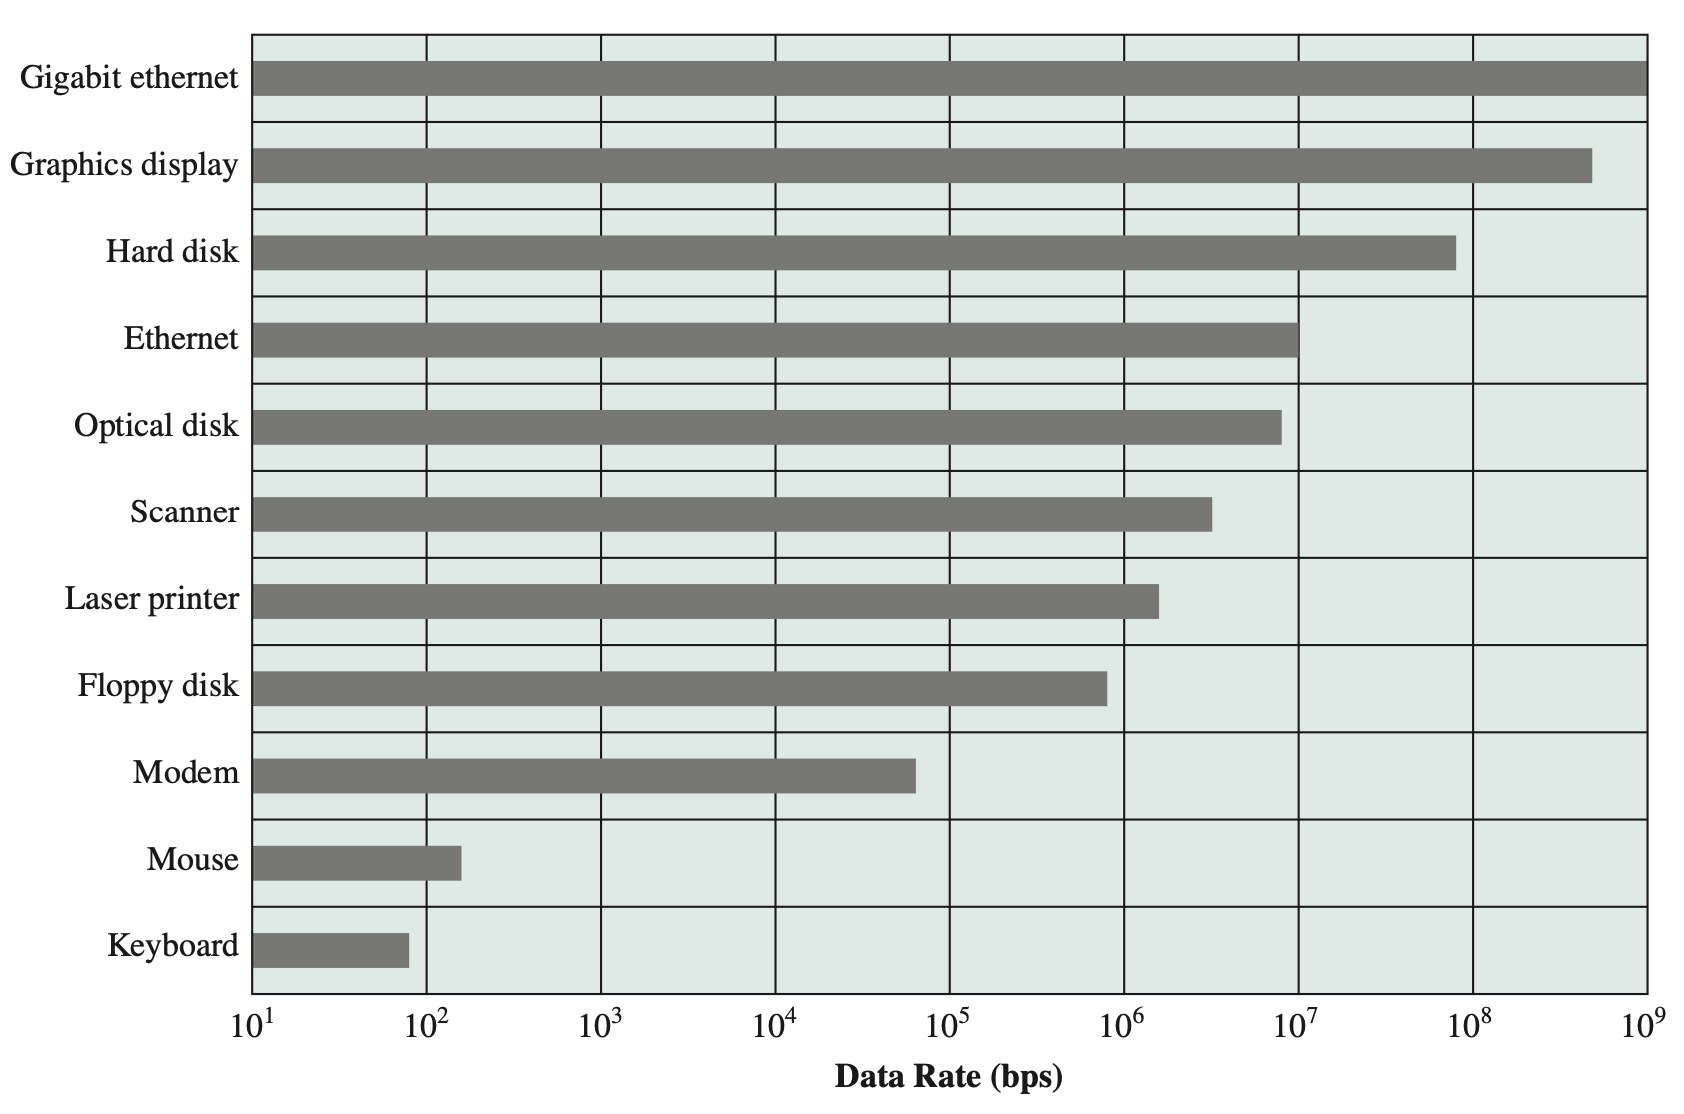
\includegraphics[width=0.6\textwidth]{img/4.1.1.3}
	\end{figure}
	\begin{itemize}
		\item 对设备进行抽象,屏蔽设备的物理细节和操作过程,配置驱动程序,提供统一界面,供用户或高层软件使用
		\begin{itemize}
			\item 抽象为裸设备:不被操作系统直接管理,由应用程序读写,I/O 效率更高
			\item 抽象为设备文件:文件系统中的节点,统一管理
		\end{itemize}
	\end{itemize}

	\subsubsection{设备管理的功能}
	\begin{itemize}
		\item 设备中断处理
		\item 缓冲区管理
		\item 设备的分配和去配
		\item 设备驱动调度
		\item 实现虚拟设备
	\end{itemize}

	\subsubsection{设备管理的层次}
	\begin{itemize}
		\item I/O 硬件:I/O 设备及其接口线路、控制部件、通道
		\item I/O 软件:系统 I/O 软件、用户空间 I/O 软件
	\end{itemize}

	\subsection{I/O控制方式}
	\subsubsection{设备控制器}
	\begin{itemize}
		\item 为达到模块化和通用性的设计目标,通常将 I/O 设备中的机械部件和电子部件分开处理
		\begin{itemize}
			\item 机械部件是指设备本身
			\item 电子部件称为设备控制器
			\begin{itemize}
				\item 又称为设备适配器、I/O 控制器、I/O 控制接口,简称 I/O 模块或 I/O接口
			\end{itemize}
		\end{itemize}
		\item 操作系统与设备控制器交互,而非与设备交互
		\begin{itemize}
			\item 多数微型和小型计算机系统通过单总线模式来交互
			\item 大中型计算机采用多总线结构和多通道方式来交互
		\end{itemize}
		\item 设备控制器具体控制设备进行 I/O,将串行的位流装配成字节,存入控制器内部的缓冲区形成字节块,在校验和确认无错后,这块数据将被复制进入内存
		\item 设备控制器的功能:CPU 与设备之间的接口
		\begin{itemize}
			\item 接收和识别 CPU 或通道发来的命令
			\item 实现数据交换
			\item 发现和记录设备及自身的状态信息,供 CPU 处理使用
			\item 当连接多台设备时,识别设备地址
		\end{itemize}
		\item 设备控制器的组成部分
		\begin{itemize}
			\item 状态/控制寄存器
			\item 数据缓冲寄存器
			\item 地址译码器和 I/O 控制逻辑
			\item 外设接口控制逻辑
		\end{itemize}
	\end{itemize}

	\begin{figure}[H]
		\centering
		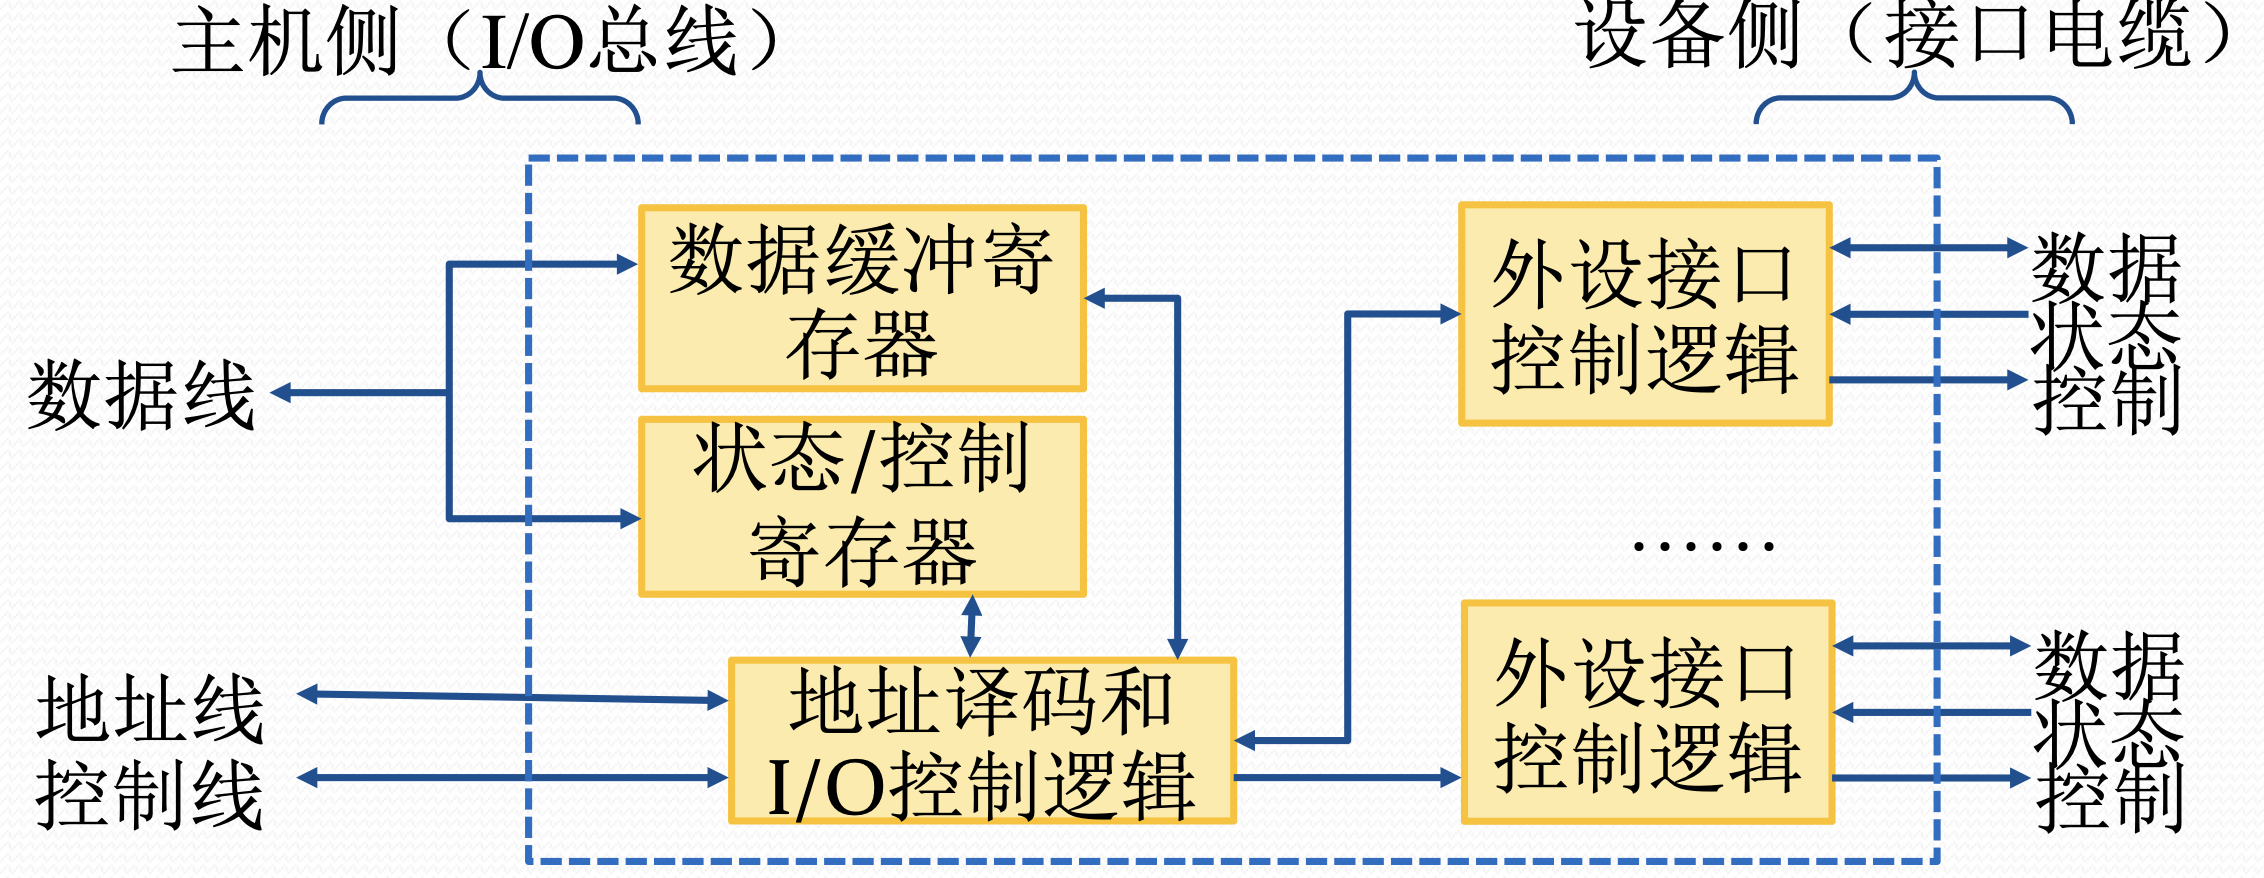
\includegraphics[width=0.6\textwidth]{img/4.1.2.1}
	\end{figure}

	\subsubsection{I/O控制方式}
	I/O 控制方式可分为4类:轮询方式、中断方式、DMA 方式和通道方式
	\begin{itemize}
		\item 它们的差别在于 CPU 与设备并行工作的方式和程度不同
		\item 轮询方式中 CPU 全程参与 I/O 操作
		\item 中断方式相比轮询方式减少了 CPU 参与 I/O 操作的工作
		\item DMA 与通道方式可以在没有 CPU 参与的情况下完成 I/O 操作
		\begin{itemize}
			\item 该过程将 CPU 从 I/O 操作中彻底解放出来,从而消除了系统性能瓶颈
		\end{itemize}
	\end{itemize}

	\subsubsection{轮询方式}
	轮询方式的处理流程:

	\begin{figure}[H]
		\centering
		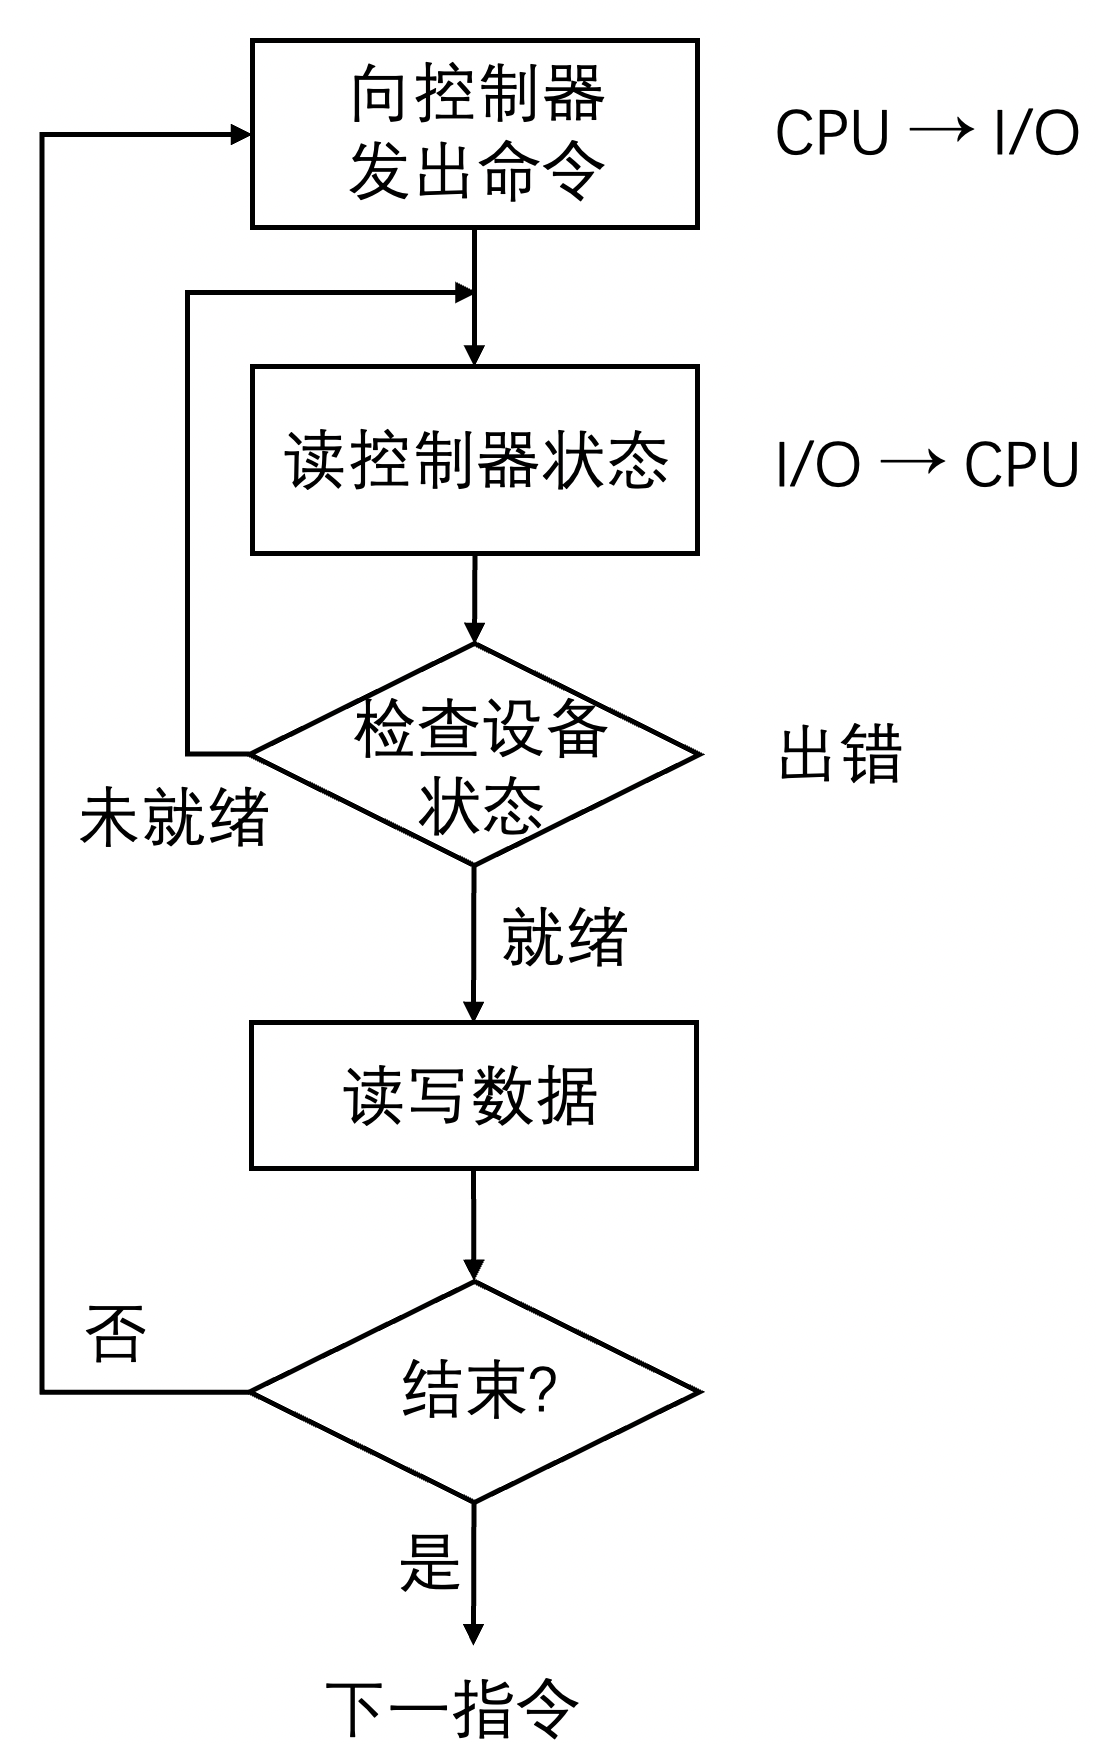
\includegraphics[width=0.23\textwidth]{img/4.1.2.3}
	\end{figure}
	\begin{itemize}
		\item 处理器向控制器发送一个 I/O 命令
		\item 如果设备未就绪,则重复测试过程,直至设备就绪
		\item 执行数据交换
		\item 等待 I/O 操作完成后,才可以继续其它操作
	\end{itemize}

	轮询方式的特点:
	\begin{itemize}
		\item 处理 I/O 请求会终止原程序的执行
		\item CPU 需要等待 I/O 设备就绪
		\item CPU 需要参与数据传送
		\item CPU 和设备只能串行工作,效率低下
	\end{itemize}


	\subsubsection{中断方式}
	中断方式的处理流程:
	\begin{figure}[H]
		\centering
		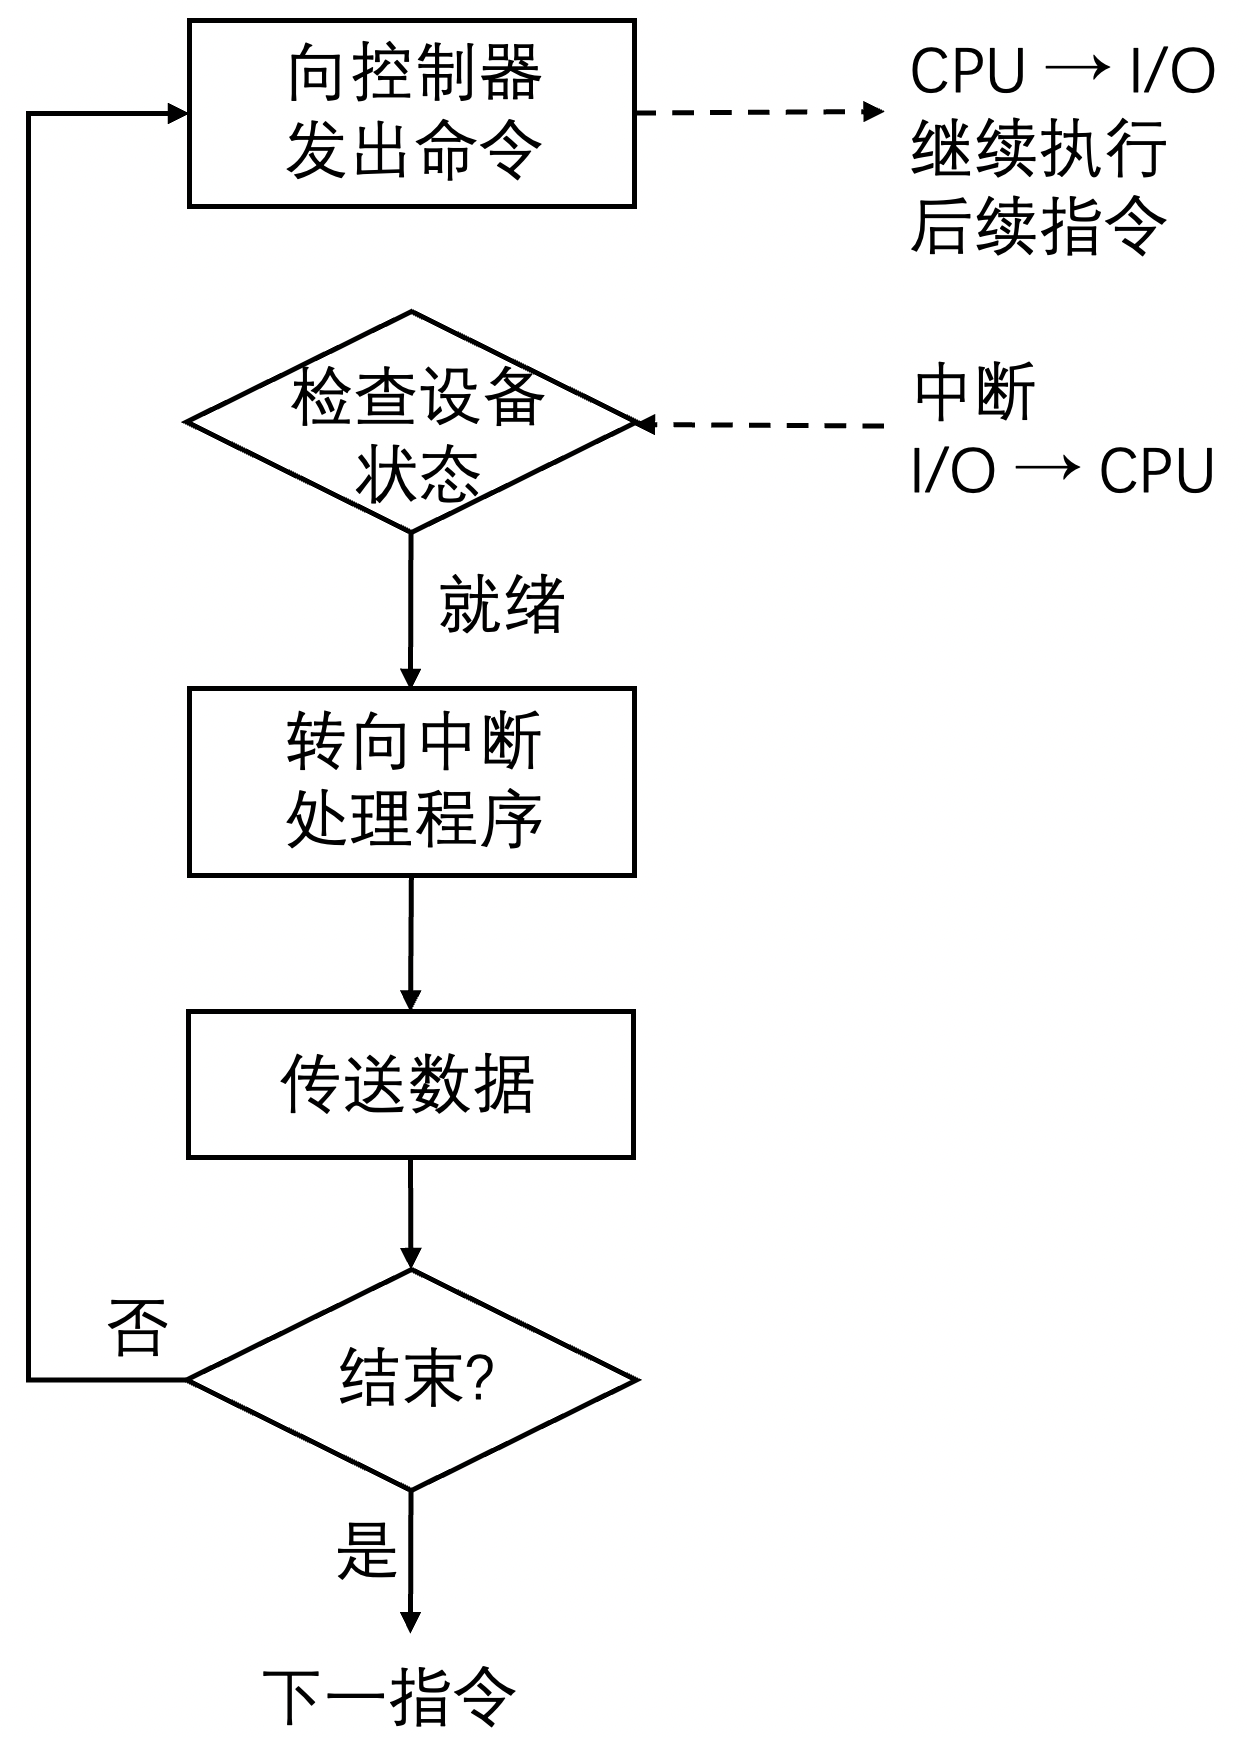
\includegraphics[width=0.3\textwidth]{img/4.1.2.4}
	\end{figure}
	\begin{itemize}
		\item 处理器向控制器发出一个 I/O 命令,然后继续执行后续指令
		\begin{itemize}
			\item 如果该进程不需要等待 I/O 完成, 后续指令可以仍是该进程中的指令
			\item 否则,该进程在这个中断上挂起, 处理器执行其他工作
		\end{itemize}
		\item 控制器检查设备状态,就绪后发起中断
		\item CPU 响应中断,转向中断处理程序
		\item 中断处理程序执行数据读写操作
		\item 恢复执行原先的程序
	\end{itemize}

	中断方式的特点:
	\begin{itemize}
		\item 响应中断后会终止原程序的执行
		\item CPU 不需要等待 I/O 设备就绪
		\item CPU 需要参与数据传送
		\item CPU 和设备部分并行操作,效率有所提高
	\end{itemize}

	\subsubsection{DMA方式}
	DMA模块:模仿处理器来控制主存和设备控制器之间的数据交换
	\begin{itemize}
		\item 内存地址寄存器:存放内存中需要交换数据的地址,DMA 传送之前由程序送入首地址;DMA 传送过程中,每次交换数据都把地址寄存器的内容加 1
		\item 字计数器:记录传送数据的总字数,每次传送一个字就把字计数器减 1
		\item 数据缓冲寄存器或数据缓冲区:暂存每次传送的数据
		\item 设备地址寄存器:存放 I/O 信息的地址,如磁盘的柱面号、磁头号、扇区号
		\item 中断机制和控制逻辑:用于向 CPU 提出 I/O 中断请求及保存 CPU 发来的 I/O 命令,管理 DMA 的传送过程
		\begin{itemize}
			\item DMA 与内存之间采用字传送,DMA 与设备之间可能是字位或字节传送,所以 DMA 中要设置数据移位寄存器、字节计数器等硬件逻辑
		\end{itemize}
	\end{itemize}
	\begin{figure}[H]
		\centering
		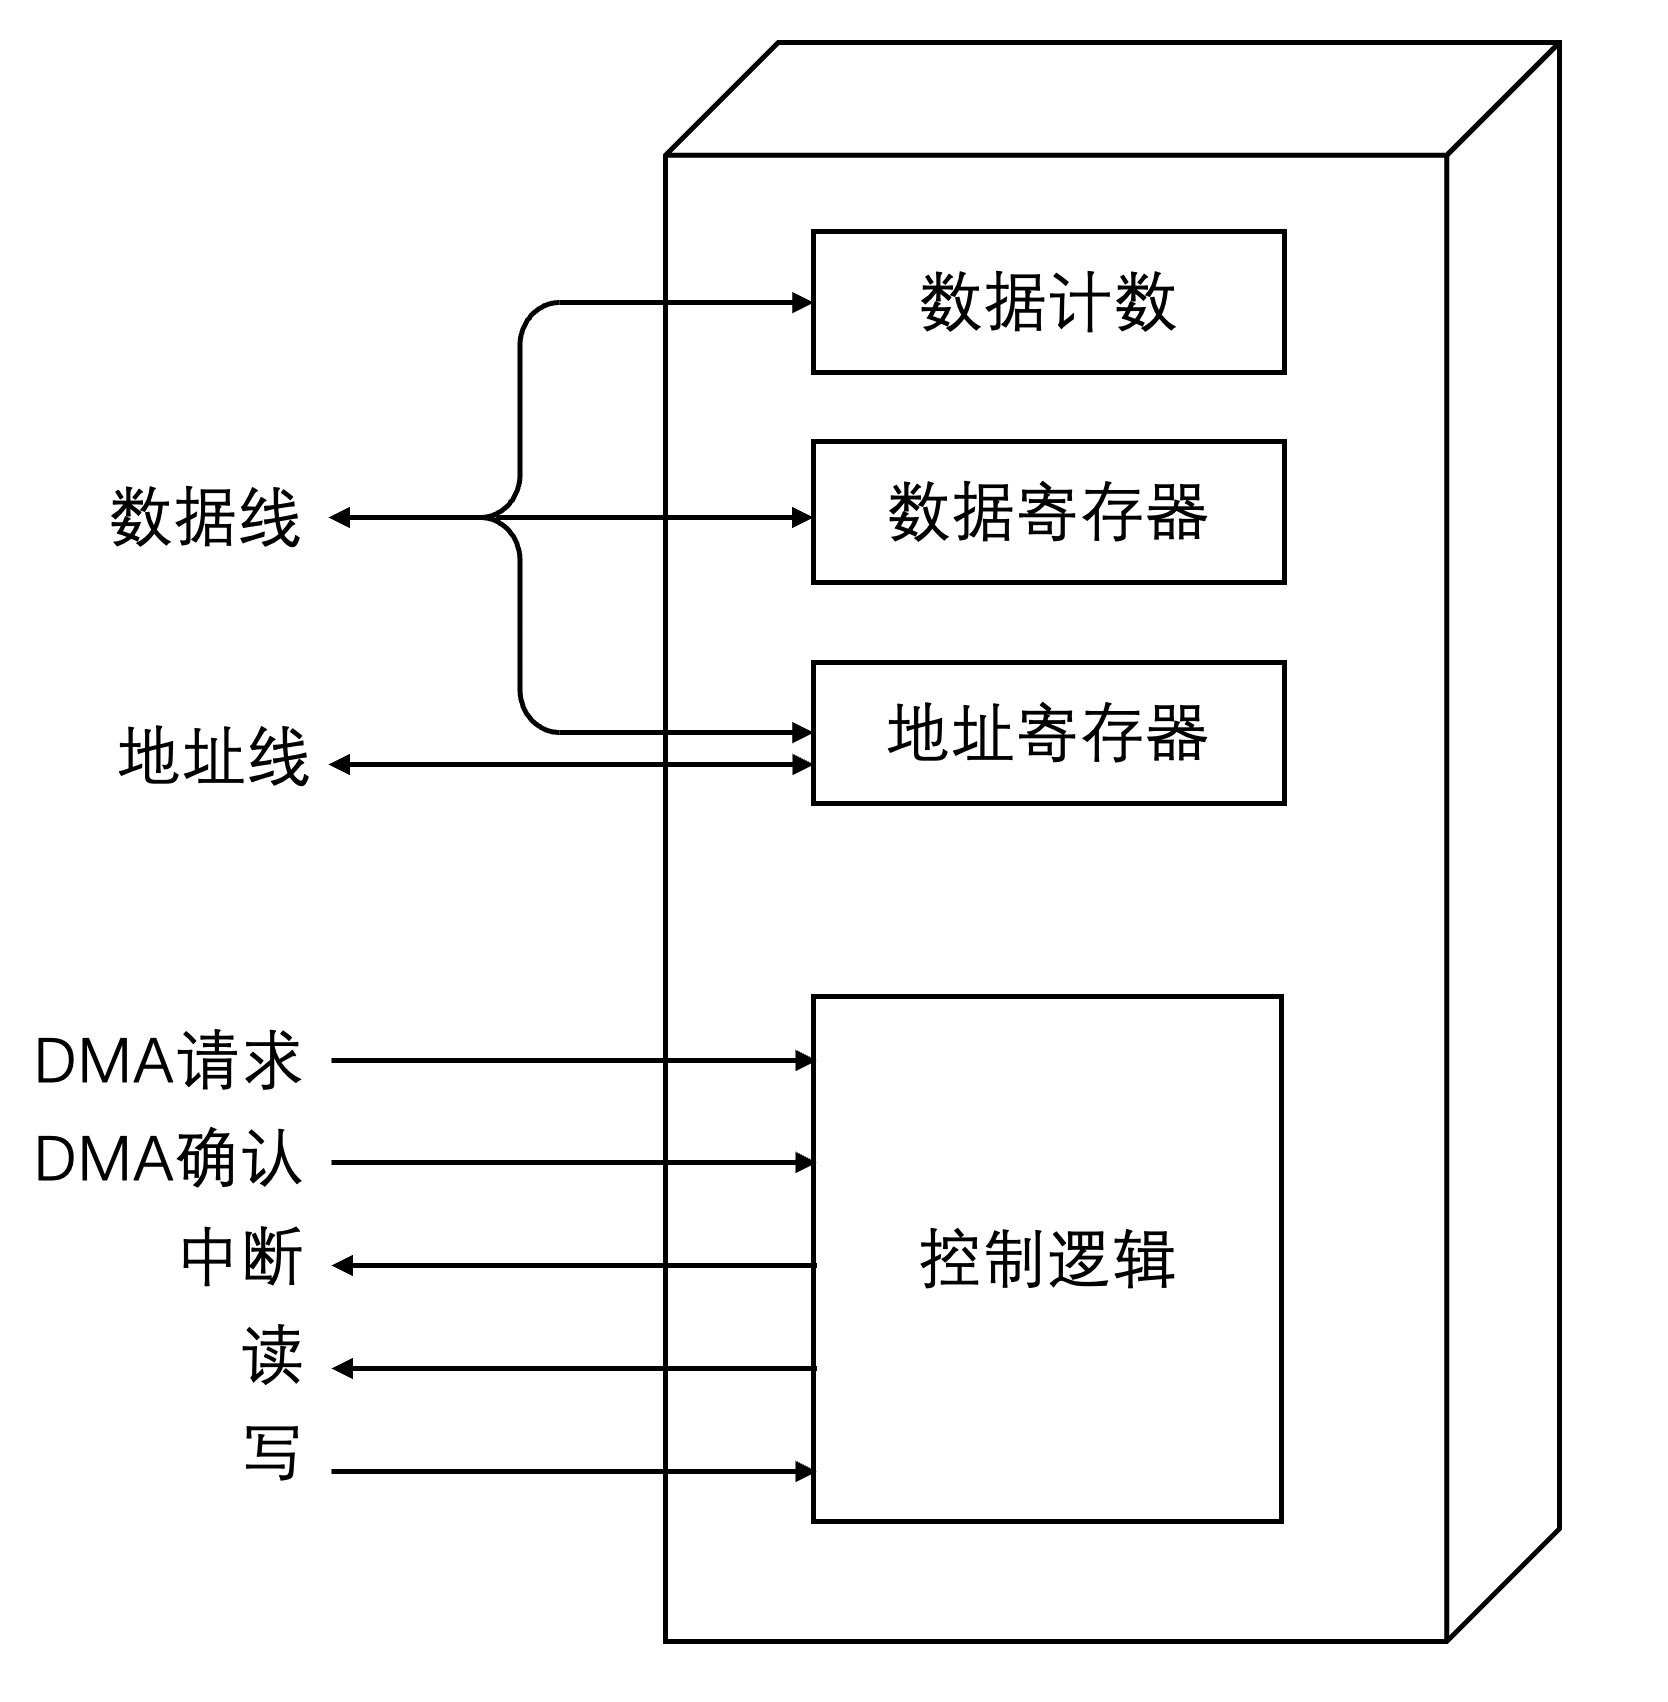
\includegraphics[width=0.4\textwidth]{img/4.1.2.5}
	\end{figure}

	DMA 方式的处理流程:
	\begin{figure}[H]
		\centering
		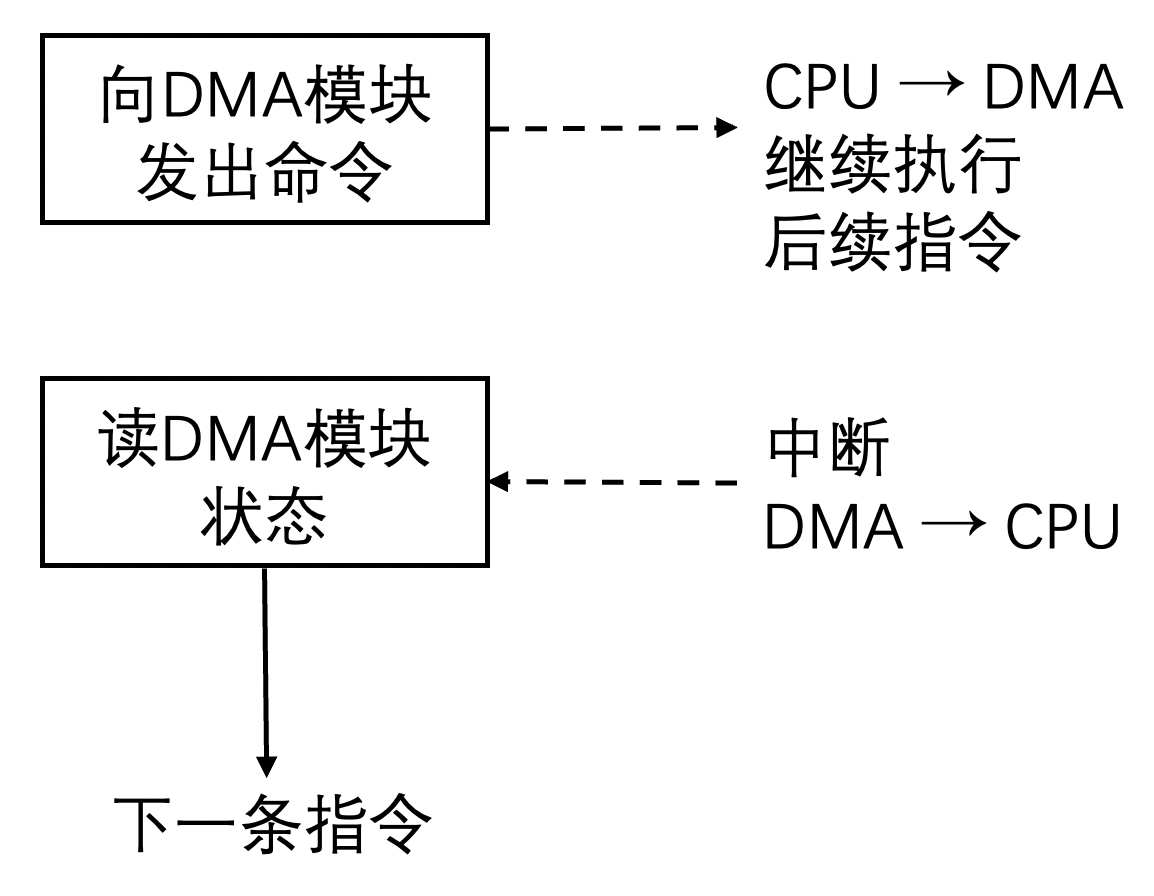
\includegraphics[width=0.3\textwidth]{img/4.1.2.5.1}
	\end{figure}
	\begin{itemize}
		\item 处理器向 DMA 模块发出 I/O 命令
		\item 处理器继续执行其它工作,DMA 模块负责传送全部数据
		\item 数据传送结束后,DMA 中断处理器
	\end{itemize}

	DMA 方式的特点:
	\begin{itemize}
		\item CPU 不会终止原程序的执行
		\item CPU 只在数据传送的开始和结束时参与
		\begin{itemize}
			\item 开始时,CPU 需要对 DMA 模块进行初始化
			\item 结束时,CPU 响应中断,但不必保存现场
		\end{itemize}
	\end{itemize}

	DMA 方式中的周期窃取
	\begin{itemize}
		\item 当 DMA 和 CPU 同时经总线访问内存时,CPU 总是将总线的占有权让给 DMA 一个或几个主存周期,一般是一个存取周期,让设备和内存之间交换数据
		\item 周期窃取对延迟 CPU 与主存的数据交换影响不大
		\begin{itemize}
			\item 数据传送过程是不连续的和不规则的
			\item CPU 大部分情况下与 Cache 进行数据交换,直接访问内存较少
		\end{itemize}
	\end{itemize}
	\begin{figure}[H]
		\centering
		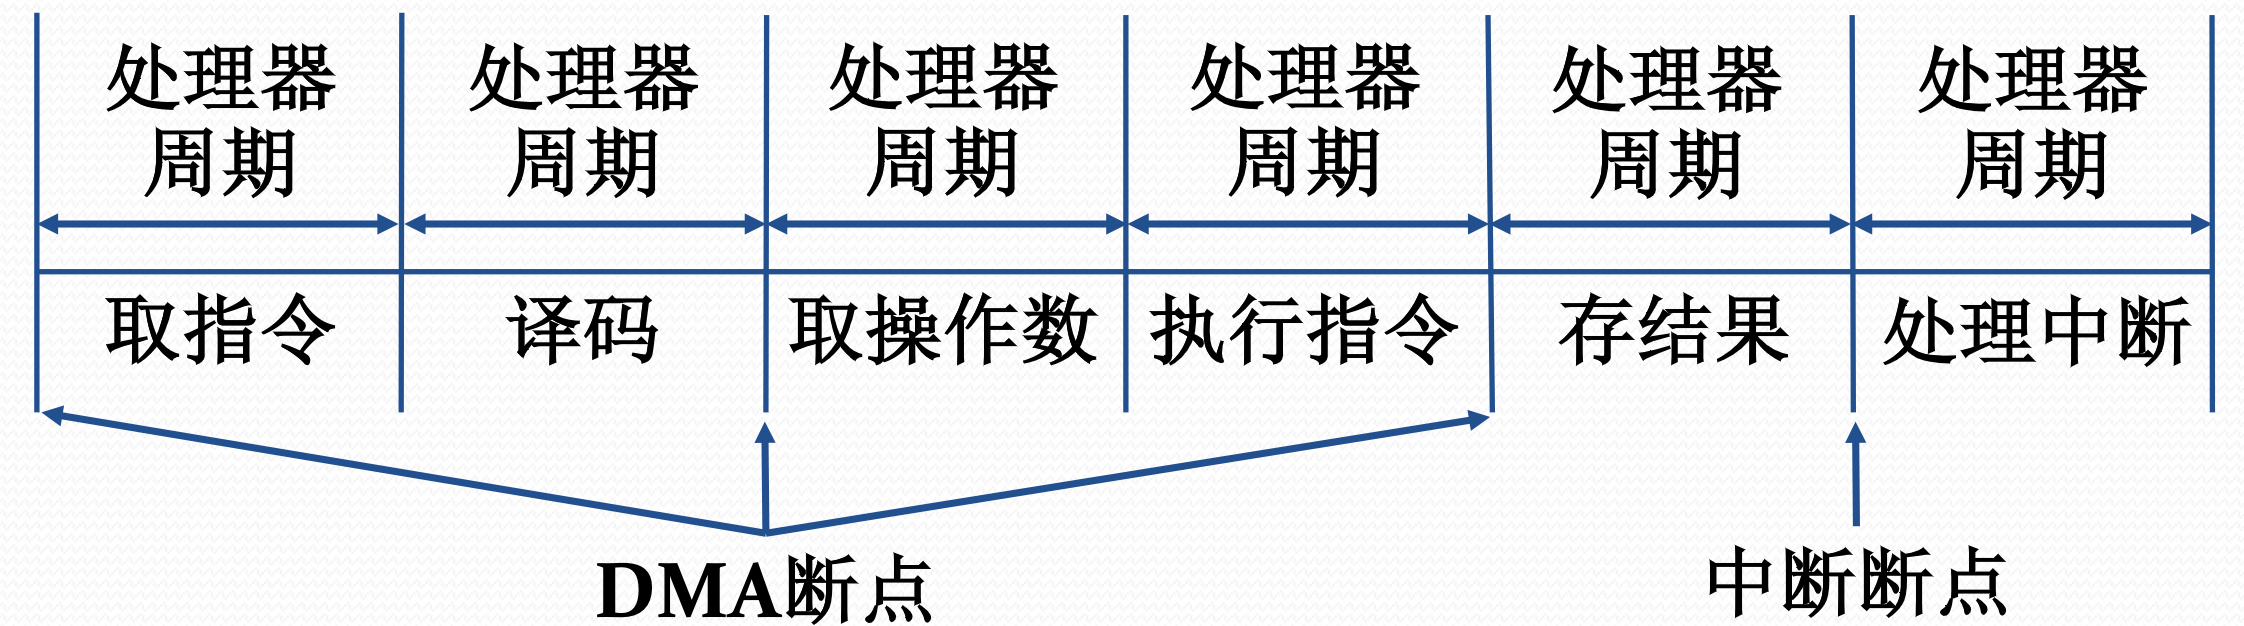
\includegraphics[width=0.75\textwidth]{img/4.1.2.5.2}
	\end{figure}
	轮询方式、中断方式和 DMA 方式的比较
	\begin{table}[H]
		\centering
		\begin{tabular}{|c|c|c|}
		\hline
		CPU作用 & 等待设备 & 数据传送 \\ \hline
		轮询方式  & 需要   & 参与   \\ \hline
		中断方式  & 不需要  & 参与   \\ \hline
		DMA方式 & 不需要  & 不参与  \\ \hline
		\end{tabular}
	\end{table}

	\subsubsection{通道方式}
	I/O 通道又称为通道控制器、I/O 处理器,用于完成逻辑上独立的 I/O 任务,适用于中大型计算机系统

	设备控制器包含自身专用的处理器和通道程序,自成体系,使得 CPU 与通道高度并行,实现通道和 CPU 并行操作,通道之间并行操作,设备之间并行操作
	\begin{itemize}
		\item 处理器可以不再执行琐碎的 I/O 命令,而改为在主存中组织通道程序,由通道来执行逻辑的 I/O 任务
		\item 采用主存,通道,控制器,设备的四级连接,实施三级控制,可控制多台同类或不同类的设备
		\begin{itemize}
			\item 一个 CPU 通常连接多个通道,通过 I/O 指令控制
			\item 一个通道可以连接若干控制器,通过执行通道命令控制
			\item 一个控制器可以连接若干设备,通过动作序列控制
		\end{itemize}
	\end{itemize}

	DMA 和 I/O 通道的不同点:DMA 中,每一个 I/O 指令只能读写一个数据块;而通道可以一次面向不同的多个数据块

	I/O 通道的工作流程:
	\begin{itemize}
		\item CPU 在执行主程序时遇到 I/O 任务,启动指定通道(通过通道程序地址字 CAW)上选址的设备
		\item 启动成功,通道开始控制设备进行操作,此时 CPU 继续执行其他任务,直到 I/O 操作完成
		\item 通道发出 I/O 操作结束中断,处理器相应并停止当前工作,转向处理 I/O 操作结束事件
	\end{itemize}

	\subsection{总线与I/O}
	\subsubsection{单总线}
	将 CPU、主存和 I/O 模块连接到同一组总线上
	\begin{itemize}
		\item 优点:结构简单,易于扩充
		\item 缺点:主存需要和 I/O 模块共用总线;设备增多会造成总线变长,进而增加传输时延;无法适用于大量高速设备
	\end{itemize}
	\begin{figure}[H]
		\centering
		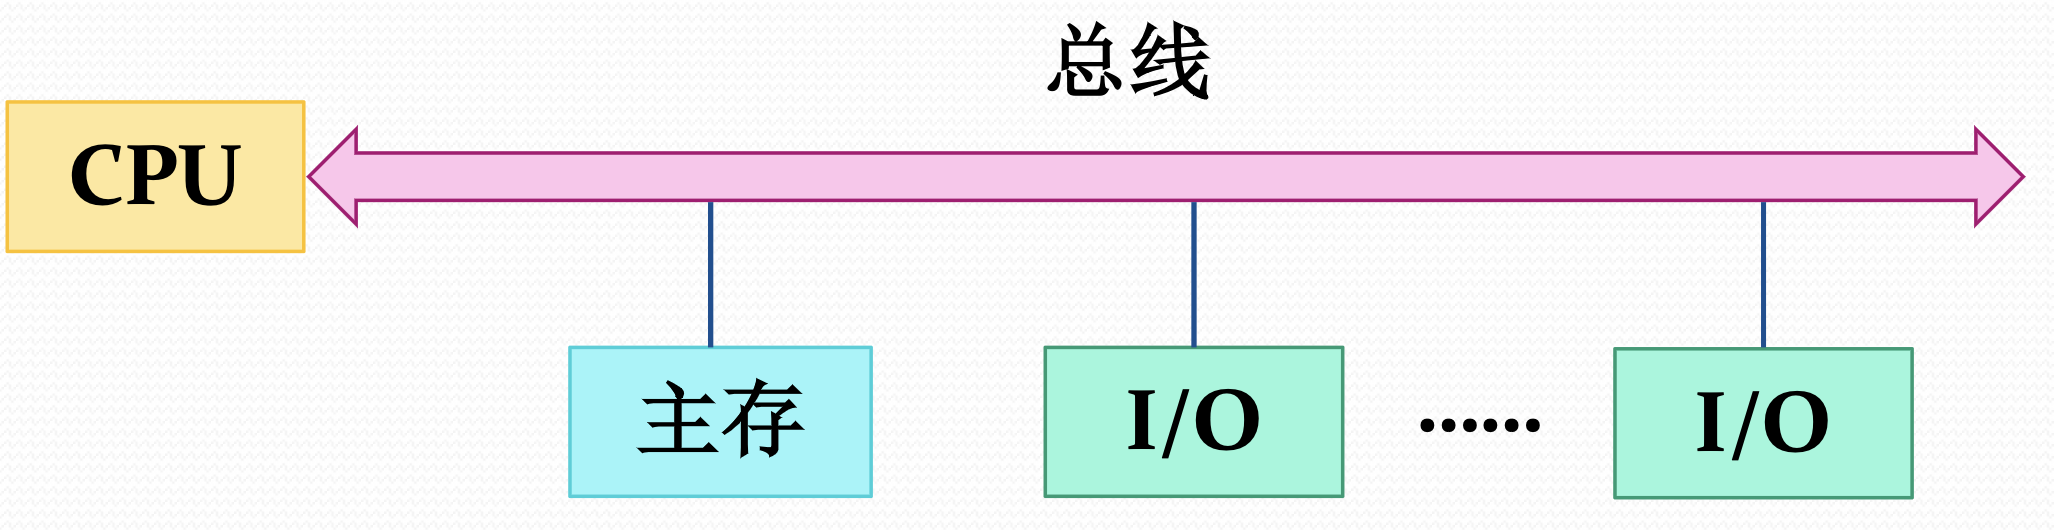
\includegraphics[width=0.5\textwidth]{img/4.1.3.1}
	\end{figure}

	\subsubsection{传统的三级总线}
	主存和 Cache 通过主存总线传送数据,主存总线和扩展总线上的 I/O 设备之间传送数据通过扩展总线接口缓冲
	\begin{itemize}
		\item 优点:主存与 I/O 之间的数据传送与处理器的活动分离;可以支持更多的 I/O 设备
		\item 缺点:不适用于 I/O 设备数据速率相差太大的情形
	\end{itemize}
	\begin{figure}[H]
		\centering
		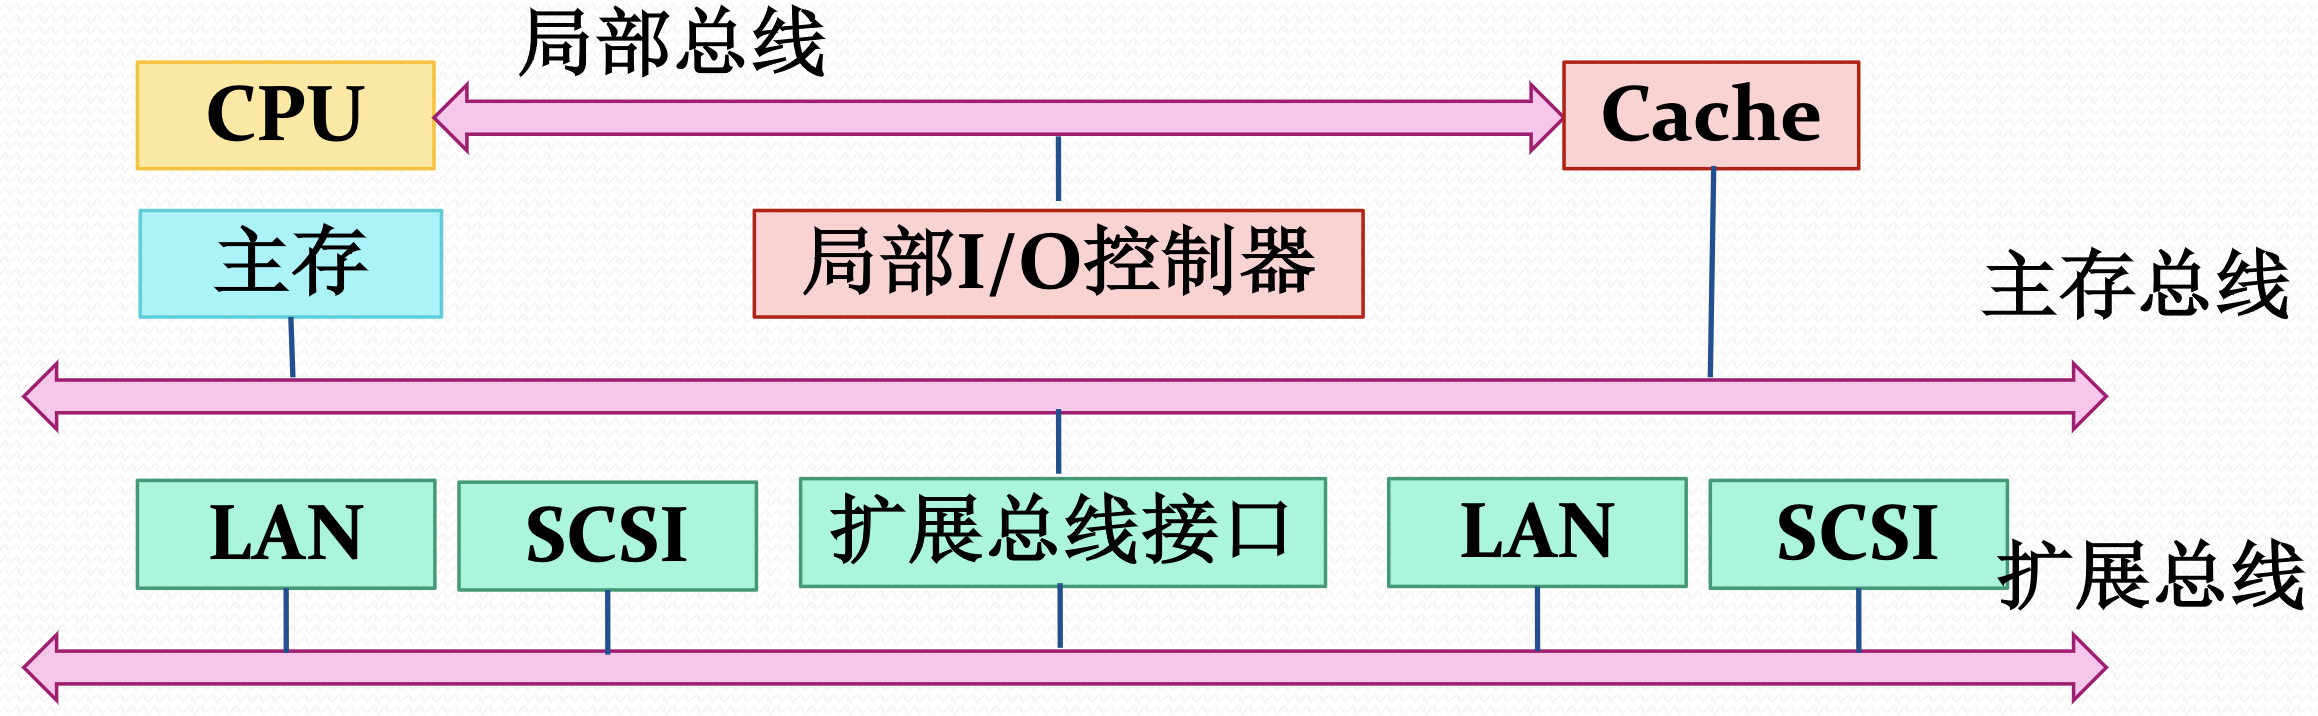
\includegraphics[width=0.6\textwidth]{img/4.1.3.2}
	\end{figure}

	\subsubsection{采用南北桥的多级总线}
	通过存储总线、PCI 总线、E(ISA) 总线分别连接主存、高速 I/O 设备和低速 I/O 设备,可以支持不同数据速率的 I/O 设备

	\subsubsection{采用I/O通道的多级总线}
	支持 CPU、主存和多个 I/O 通道之间的数据传送;支持 I/O 通道和 I/O 控制器,以及 I/O 控制器和设备之间的数据传送
	\begin{figure}[H]
		\centering
		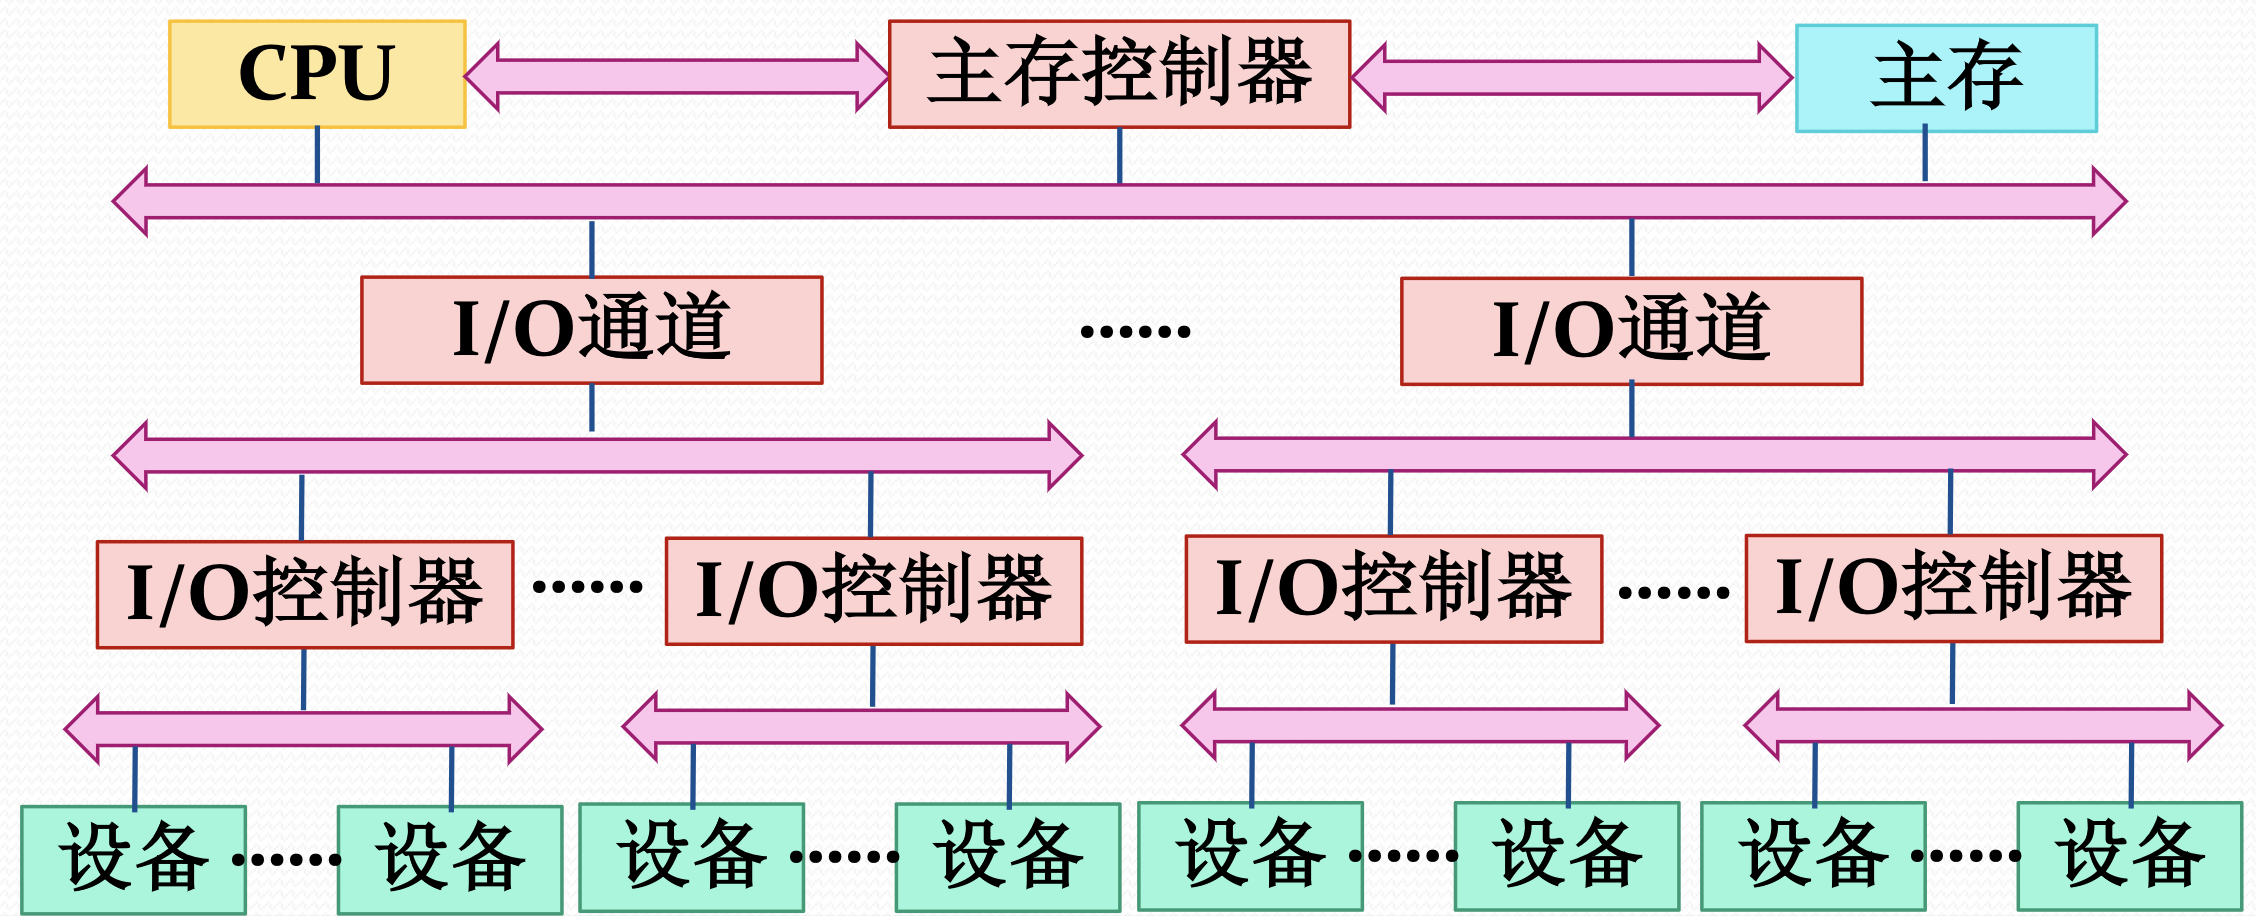
\includegraphics[width=0.7\textwidth]{img/4.1.3.4}
	\end{figure}


	\section{设备管理软件}
	\subsection{I/O软件的实现层次}

	\subsubsection{I/O软件设计目标和原则}
	I/O 软件的总体设计目标是高效率和通用性
	\begin{itemize}
		\item 高效率:改善设备效率,尤其是磁盘 I/O 操作的效率,有很大的影响
		\item 通用性:用统一的标准来管理所有设备
	\end{itemize}

	I/O 软件设计思路:把软件组织成层次结构,低层软件用来屏蔽硬件细节,高层软件向用户提供简洁、友善的界面

	I/O 软件主要考虑的问题:
	\begin{itemize}
		\item 设备无关性:编写访问文件的程序与物理设备无关
		\item 出错处理:低层软件能处理的错误不让高层软件感知
		\item 同步/异步传输:支持阻塞和中断驱动两种工作方式
		\begin{itemize}
			\item 同步:如果要同步就需要做等待,增加延迟
			\item 异步:可以不等待,提供并行度(不等是有前提的,运行进程的后续操作不可以依赖 I/O 操作的结果)
		\end{itemize}
		\item 缓冲技术:建立数据缓冲区,匹配数据的到达率与离去率,提高吞吐率
	\end{itemize}

	\subsubsection{I/O软件的层次结构}
	\begin{figure}[H]
		\centering
		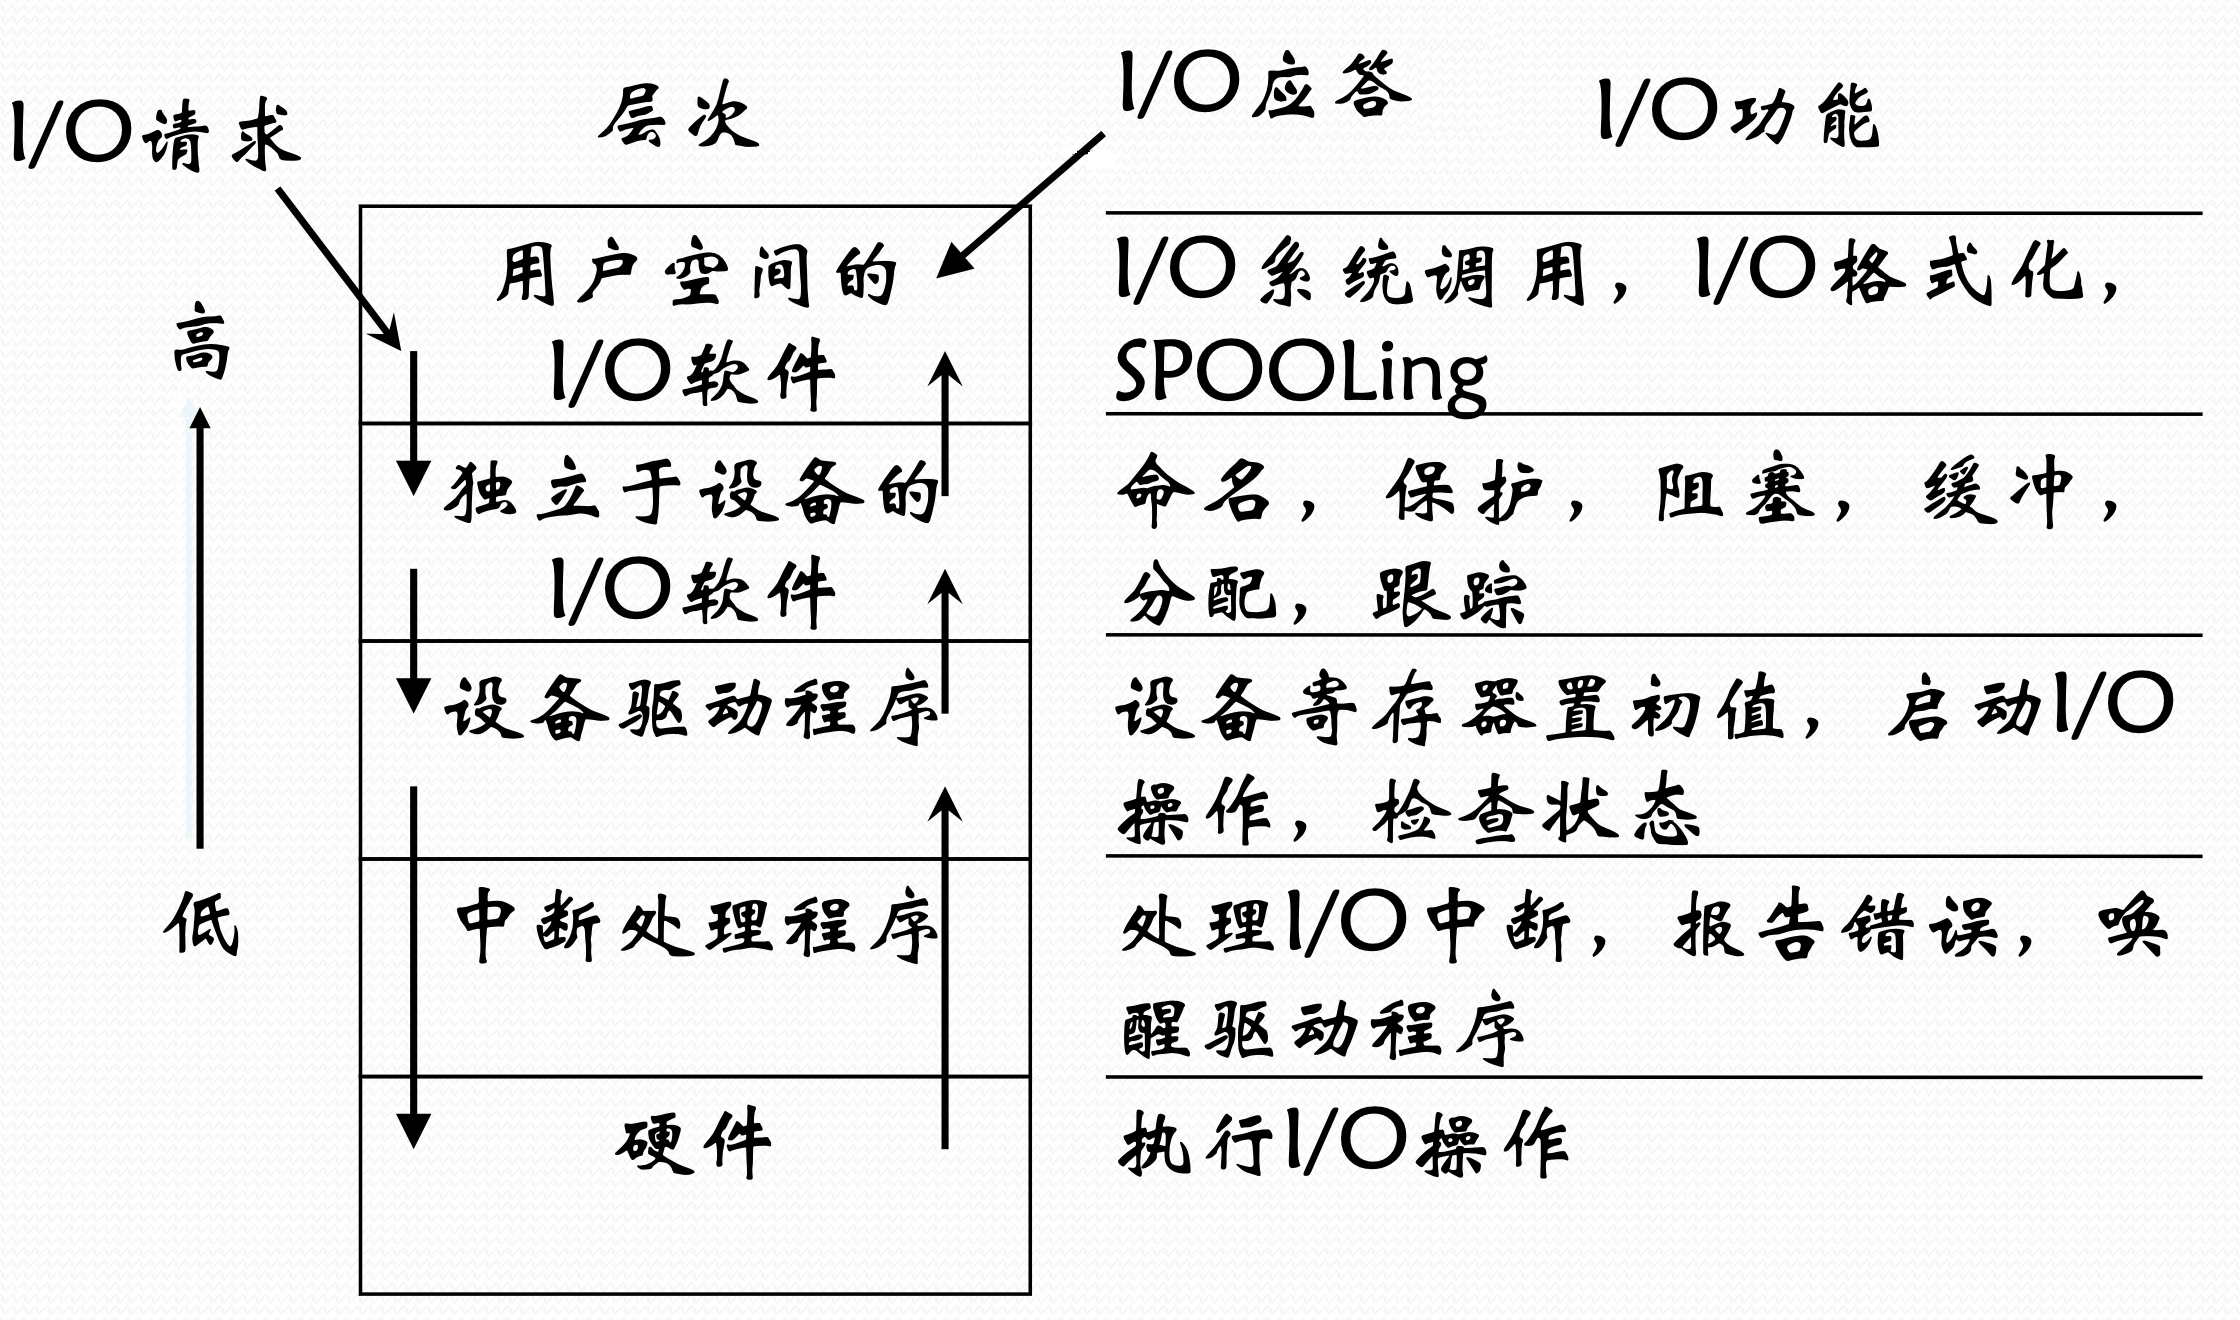
\includegraphics[width=0.6\textwidth]{img/4.2.1.2}
	\end{figure}

	\subsection{I/O软件的实现}

	\subsubsection{I/O中断处理程序}
	\begin{itemize}
		\item I/O 中断处理程序位于操作系统底层,与硬件设备密切相关,与系统其余部分尽可能少地发生联系
		\item 进程请求 I/O 操作时,通常被挂起,直到数据传输结束后并产生 I/O 中断时,操作系统接管 CPU 后转向中断处理程序
		\item 当设备向 CPU 提出中断请求时,CPU 响应请求并转入中断处理程序
		\item I/O 中断处理程序的功能
		\begin{itemize}
			\item 检查设备状态寄存器内容,判断产生中断的原因,根据 I/O 操作的完成情况进行相应的处理
			\item 如果数据传输有错,向上层软件报告设备的出错信息,实施重新执行
			\item 如果正常结束,唤醒等待传输的进程,使其转换为就绪态
			\item 如果有等待传输的 I/O 命令,通知相关软件启动下一个 I/O 请求
		\end{itemize}
	\end{itemize}

	\subsubsection{I/O设备驱动程序}
	I/O 设备驱动程序包括与设备密切相关的所有代码
	\begin{itemize}
		\item 从独立于设备的软件中接收并执行 I/O 请求
		\begin{itemize}
			\item 把用户提交的逻辑 I/O 请求转化为物理 I/O 操作的启动和执行
			\item 监督设备是否正确执行,管理数据缓冲区,进行必要的纠错处理
		\end{itemize}
	\end{itemize}

	I/O 设备驱动程序的功能
	\begin{itemize}
		\item 设备初始化
		\begin{itemize}
			\item 在系统初次启动或设备传输数据时,预置设备和控制器以及通道状态
		\end{itemize}
		\item 执行设备驱动例程
		\begin{itemize}
			\item 负责启动设备,进行数据传输
			\item 对于具有通道方式,还负责生成通道指令和通道程序,启动通道工作
		\end{itemize}
		\item 调用和执行中断处理程序
		\begin{itemize}
			\item 负责处理设备和控制器及通道所发出的各种中断
		\end{itemize}
	\end{itemize}

	I/O 设备驱动程序的层次
	\begin{itemize}
		\item 每个设备驱动程序只处理一种设备,或者一类紧密相关的设备
		\item 设备驱动程序分为整体驱动程序和分层驱动程序
		\begin{itemize}
			\item 整体驱动程序直接向操作系统提供接口和控制硬件
			\begin{itemize}
				\item 适用于功能简单的驱动程序,效率较高,但较难迁移
			\end{itemize}
			\item 分层驱动程序将驱动程序分成多层,放在栈中,系统接到 I/O 请求时先调用栈顶的驱动程序,栈顶的驱动程序可以直接处理请求或向下调用更低层的驱动程序,直至请求被处理
			\begin{itemize}
				\item 适用于功能复杂、重用性要求较高的驱动程序,结构清晰且便于移植,但会增加一部分系统开销
			\end{itemize}
		\end{itemize}
	\end{itemize}

	\subsubsection{独立于设备的I/O软件}
	执行适用于所有设备的常用 I/O 功能,并向用户层软件提供一致性接口
	\begin{itemize}
		\item 设备命名:通过路径名寻址设备
		\item 设备保护:检查用户是否有权访问所申请设备
		\item 提供与设备无关的数据单位:向高层软件提供统一的数据尺寸
		\item 提供缓冲技术:通过缓冲消除填满速率和清空速率的影响
		\item 设备分配和状态跟踪:分配不同类型的设备
		\item 错误处理和报告:驱动程序无法处理的错误
	\end{itemize}

	\subsubsection{用户空间的I/O软件}
	库函数:一类常用的用户空间的 I/O 软件
	\begin{itemize}
		\item 一小部分 I/O 软件不在操作系统中,是与应用程序链接在一起的库函数,甚至完全由运行于用户态的程序组成
		\item 系统调用通常由库函数封装后供用户使用,封装函数只是将系统调用所用的参数放在合适位置,然后执行访管指令来陷入内核,再由内核函数实现真正的 I/O 操作
	\end{itemize}

	SPOOLing 软件:在用户空间运行的典型的系统 I/O 软件
	\begin{itemize}
		\item 在内核外运行的系统 I/O 软件,采用预输入、缓输出和井管理技术,通过创建守护进程和特殊目录解决独占型设备的空占问题
	\end{itemize}

	\subsection{I/O操作的执行步骤}
	以读操作为例
	\begin{itemize}
		\item 应用进程对已打开文件的文件描述符执行读\textbf{系统调用}(库函数)
		\item 独立于设备的 I/O 软件\textbf{检查参数}是否正确,若正确,检查\textbf{高速缓存}中有无要读取的信息块
		\begin{itemize}
			\item 若有,从缓冲区直接读至用户区,\textbf{完成I/O请求}
			\item 若数据不在缓冲区,执行物理 I/O 操作,独立于设备的 I/O 软件将设备的逻辑名转换成物理名,检查对设备操作的许可权,将 I/O 请求排队,阻塞应用进程且等待 I/O 操作完成
		\end{itemize}
		\item 内核启动设备驱动程序,分配存放读出块的缓冲区,准备接收数据并向设备控制寄存器发送启动命令,或建立 DMA 传输,启动 I/O
		\item 设备控制器操作设备,执行数据传输
		\item 当采用 DMA 控制器控制数据传输时,一旦传输完成,硬件产生 I/O 结束中断
		\item CPU 响应中断,转向磁盘中断处理程序,检查中断产生原因和设备的执行状态
		\begin{itemize}
			\item 若设备有错,向设备驱动程序发信号,检查是否能重复执行,如果允许,重发启动设备命令,再次传输;否则,向上层软件报告错误
			\item 若设备 I/O 正确完成,将数据传输到指定的用户进程空间,唤醒阻塞进程并将其放人就绪队列。然后,系统检查有无 I/O 请求在排队,若有,再启动设备,继续传输
			\item 至此,中断处理完成且返回,将成功或失败的信息逐层向上报告
		\end{itemize}
		\item 当应用进程被再次调度执行时,从 I/O 系统调用的断点处恢复执行
	\end{itemize}

	\subsection{I/O缓冲区}

	\subsubsection{I/O缓冲技术}
	缓冲区:在内存中开辟的存储区,专门用于临时存放 I/O 操作的数据

	设置 I/O 缓冲的目的
	\begin{itemize}
		\item 解决 CPU 与设备之间速度不匹配的矛盾,协调逻辑记录大小和物理记录大小不一致的问题
		\item 减少 I/O 操作对 CPU 的中断次数
		\item 放宽对 CPU 中断响应时间的要求
		\item 提高 CPU 和设备的并行性
	\end{itemize}

	实现缓冲技术的基本思想:
	\begin{itemize}
		\item 写操作:先向系统申请一个输入缓冲区,将数据送至缓冲区,直到装满或需要写存储,待适当时候系统将缓冲区内容写到设备上
		\item 读操作:先向系统申请一个输出缓冲区,系统将设备上的物理记录读至缓冲区,根据要求将当前所需要的数据从缓冲区中读出并传送给进程
	\end{itemize}

	\subsubsection{单缓冲技术}
	操作系统在主存的系统区中开设一个缓冲区
	\begin{itemize}
		\item 输入:将数据读至缓冲区,系统将缓冲区数据送至用户区,应用程序对数据进行处理,同时系统读入接下来的数据
		\item 输出:把数据从用户区复制到缓冲区,系统将数据输出后,应用程序继续请求输出
	\end{itemize}
	\begin{figure}[H]
		\centering
		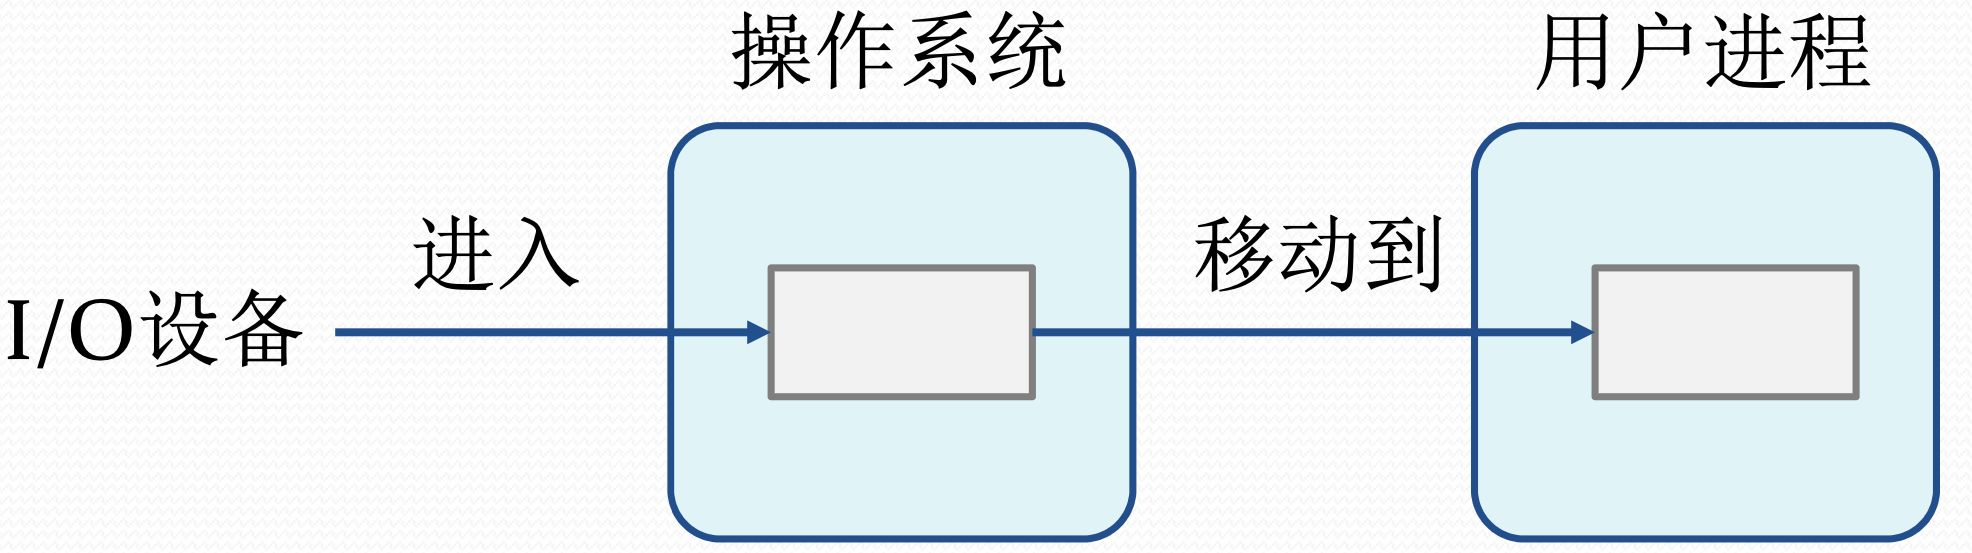
\includegraphics[width=0.5\textwidth]{img/4.2.4.2}
	\end{figure}

	\subsubsection{双缓冲技术}
	使用两个缓冲区
	\begin{itemize}
		\item 输入:设备先将数据输入缓冲区1,系统从缓冲区1把数据传到用户区,供应用程序处理,同时设备将数据传送到缓冲区2
		\item 输出:应用程序将数据从用户传送到缓冲区1,系统将数据传送到设备,同时应用程序将数据传送到缓冲区2
	\end{itemize}
	\begin{figure}[H]
		\centering
		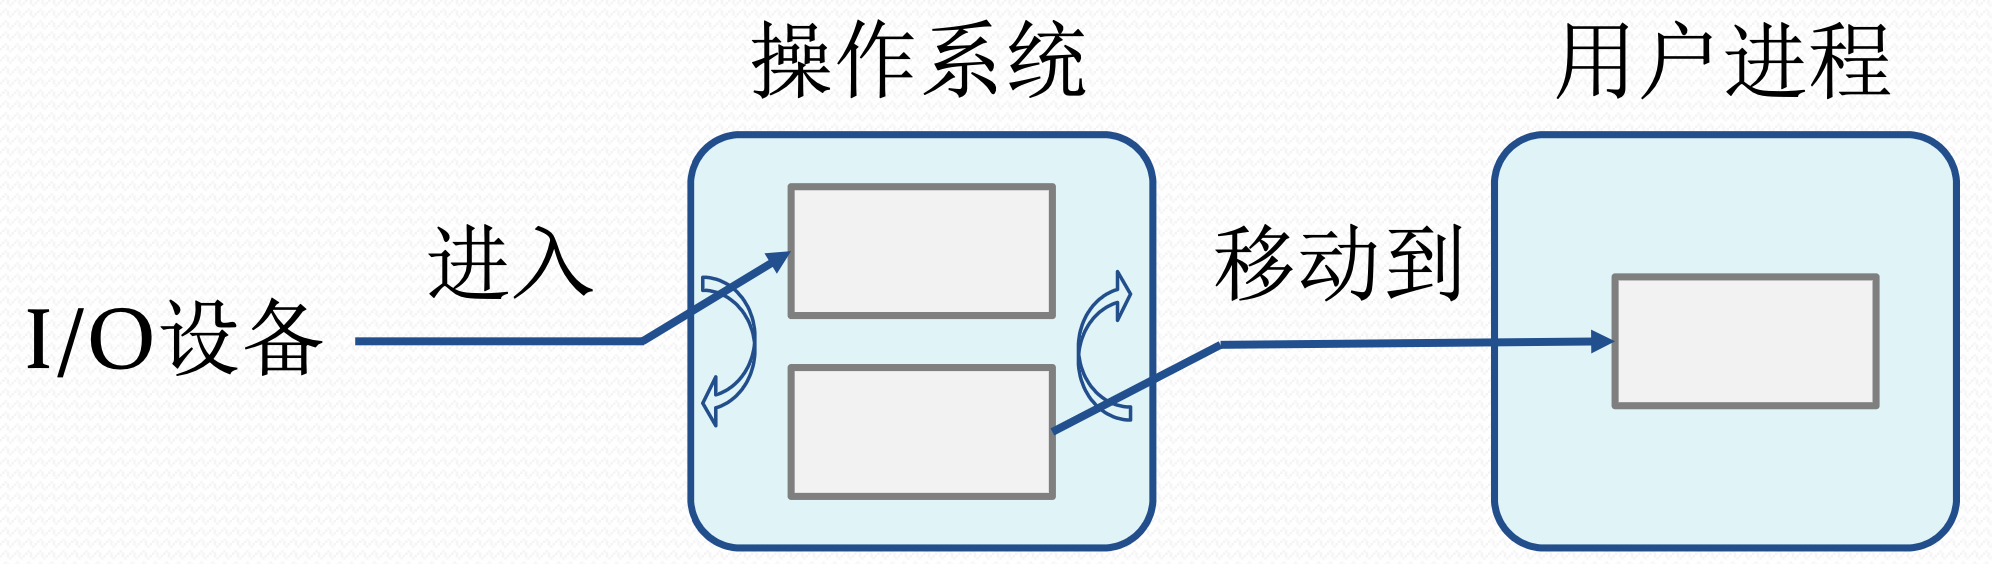
\includegraphics[width=0.5\textwidth]{img/4.2.4.3}
	\end{figure}

	\subsubsection{循环缓冲技术}
	操作系统分配一组缓冲区,每个缓冲区度有指向下一个缓冲区的链接指针,构成循环缓冲
	\begin{itemize}
		\item 解决设备和进程速度不匹配的问题
		\item 是系统的公共资源,供进程共享并由系统统一分配和管理
	\end{itemize}
	\begin{figure}[H]
		\centering
		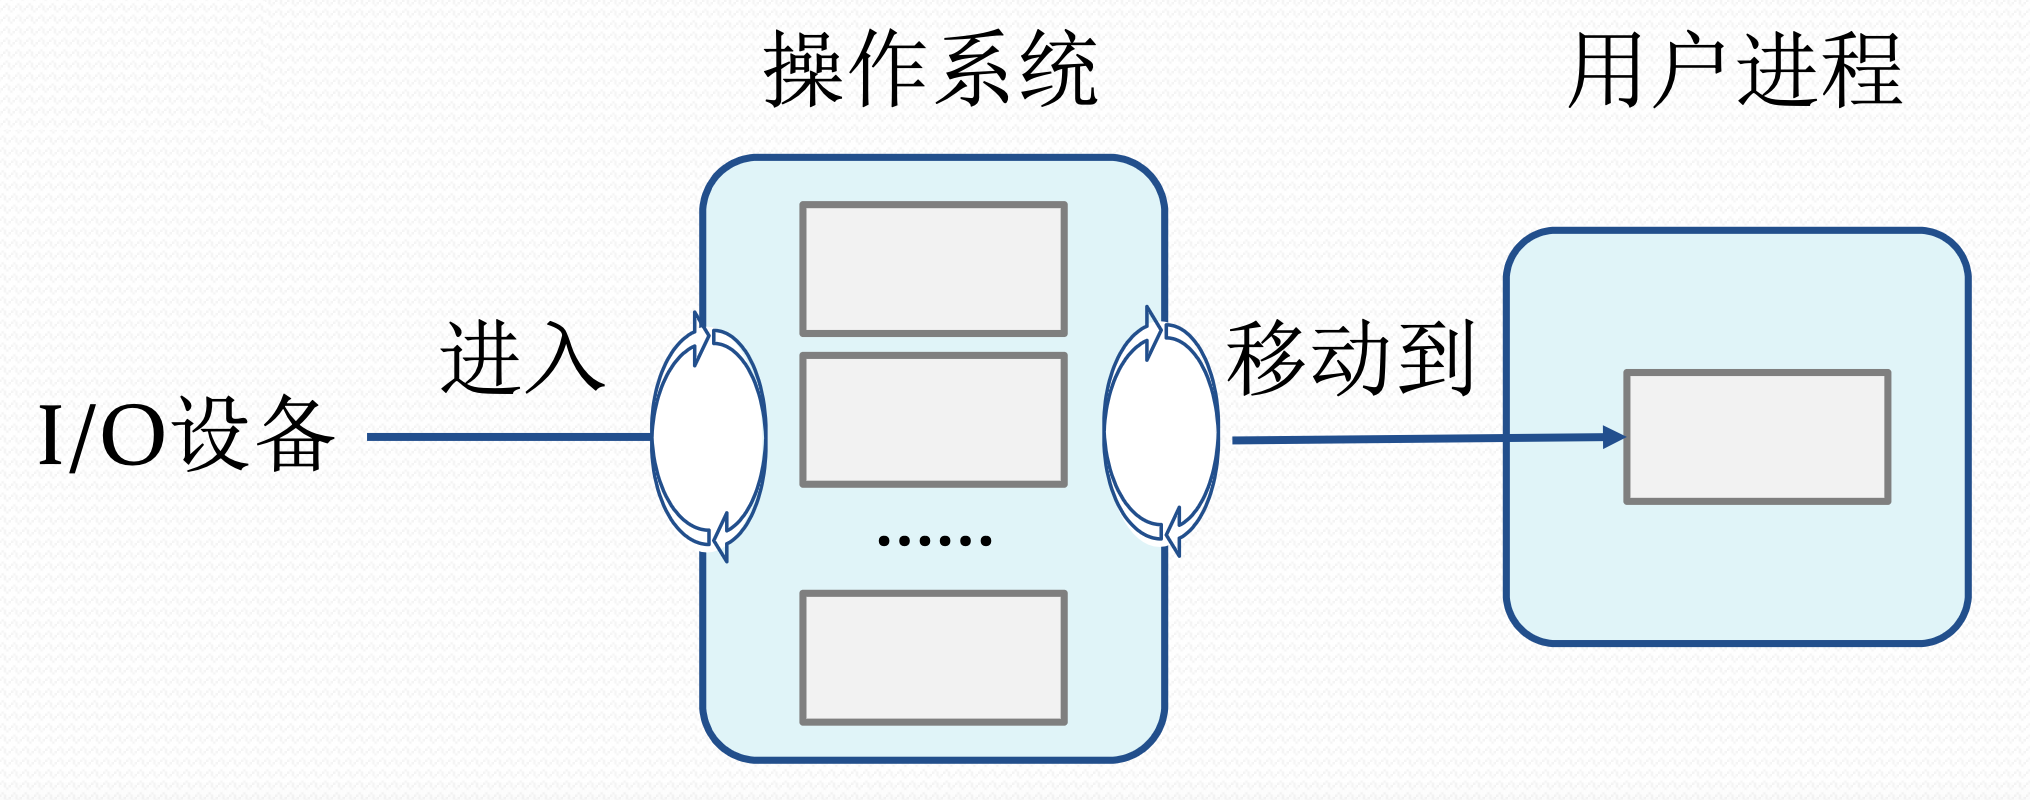
\includegraphics[width=0.5\textwidth]{img/4.2.4.4}
	\end{figure}

	\section{独占型外围设备的分配}
	\subsection{设备独立性}
	需要解决的问题:作业执行前对设备提出申请时,指定某台具体的物理设备会让设备分配变得简单,但如果所指定设备出现故障,即便计算机系统中有同类设备也不能运行

	设备独立性:用户通常不指定物理设备,而是指定逻辑设备,使得用户作业和物理设备分离开来,再通过其它途径建立逻辑设备和物理设备之间的映射
	\begin{itemize}
		\item 微型计算机的操作系统中不一定支持设备独立性
	\end{itemize}

	设备管理的功能就是将逻辑设备名转换为物理设备名,为此系统需要提供逻辑设备名和物理设备名的对应表以供转换使用
	\begin{itemize}
		\item 逻辑设备号由用户定义
		\item 物理设备号由系统规定,不可修改
	\end{itemize}

	设备独立性的优点
	\begin{itemize}
		\item 应用程序与具体物理设备无关,系统增减或变更设备时不需要修改源程序
		\item 易于应对 I/O 设备故障,提高系统可靠性
		\item 增加设备分配的灵活性,更有效地利用设备资源,实现多道程序设计
	\end{itemize}

	\subsection{独占型外设的分配}
	\subsubsection{设备分配方式}
	独占型设备:一次只能由一个进程独占使用
	\begin{itemize}
		\item 只能由一个进程独占式使用
		\item 可以让多个进程同时使用的设备称为“共享设备”,其管理工作主要是驱动调度和实施驱动,一般不必分配
	\end{itemize}

	设备分配方式
	\begin{itemize}
		\item 静态分配:进程运行前申请,实现简单,能够防止系统发生死锁,但会降低设备利用率,独占型设备多选
		\item 动态分配:进程随用随申请,提高设备利用率,但是对于打印机等独占型设备使用动态分配可以显著提高设备利用率
	\end{itemize}

	\subsubsection{独占型设备分配的数据结构}
	为实现独占型设备分配,操作系统的设备管理需要建立设备类表和设备表
	\begin{itemize}
		\item 设备类表:每类设备对应于设备类表的中的一栏
		\begin{itemize}
			\item 包括:设备类、总台数、空闲台数、设备表起始地址等
			\item 支持设备独立性时才会使用
		\end{itemize}
		\item 设备表:每类设备都有各自的设备表,用来登记这类设备中的每台物理设备
	\end{itemize}

	对于采用通道结构的系统,需要对通道、控制器和每台物理设备进行管理和控制,必须设置系统设备表、通道控制表、控制器控制表和设备控制表
	\begin{itemize}
		\item 整个系统建立一张系统设备表,记录系统配置的所有物理设备的情况,每台物理设备占有一栏
		\begin{itemize}
			\item 包括设备类型、台数、设备号、设备控制表指针等
		\end{itemize}
		\item 对于通道控制表、控制器控制表和设备控制表,每个通道、控制器、设备各设置一张
		\begin{itemize}
			\item 分别记录各自的地址(标识符)、状态(忙/闲、已分配/未分配)、等待获得此部件的进程队列指针及一次分配后相互链接的指针,以备分配和执行 I/O 操作时使用
		\end{itemize}
	\end{itemize}


	\section{共享型外围设备的驱动}
	\subsection{磁盘的物理结构}

	\subsubsection{磁盘物理结构}
	磁盘是一种直接存取存储设备,又称为随机存取存储设备,每条物理记录都有明确的位置和唯一的地址,按照三维坐标进行随机存储
	\begin{itemize}
		\item 磁盘由多个盘片组成,每个盘片被划分为多个同心圆结构的磁道,每个盘片的两面都可以存取数据
		\item 不同盘片上位于相同位置的磁道构成的圆柱体称为柱面
		\item 每个磁道分为固定多个或不等个数的扇区:为了对大量扇区寻址,操作系统将相邻的扇区组合成簇存储文件
		\item 物理块(扇面)在磁盘上的三维地址(磁头号,柱面号,扇区号)
		\begin{itemize}
			\item 盘面号也被叫做磁头号
			\item 磁道号也被叫做柱面号
			\item 面和道都是从 0 开始编址的,但扇区没有 0 扇区的概念,一定是从 1 开始编号的
		\end{itemize}
	\end{itemize}
	\begin{figure}[H]
		\centering
		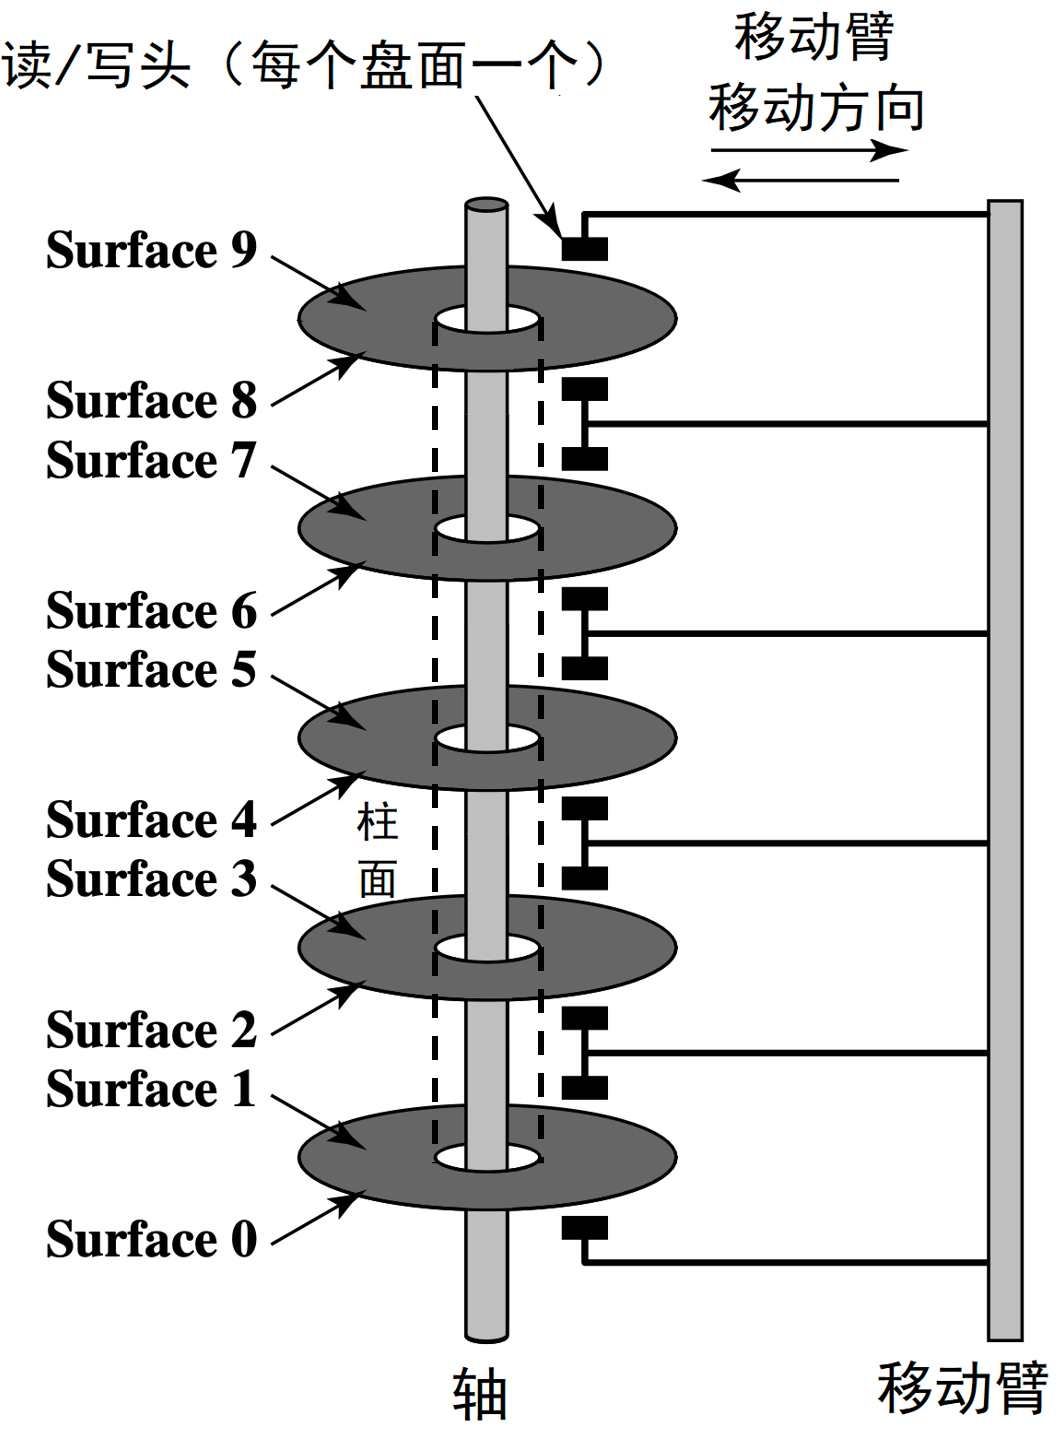
\includegraphics[width=0.4\textwidth]{img/4.4.1.1}
	\end{figure}
	
	\subsubsection{磁盘读写时间}
	读写数据时,磁头必须定位到指定的磁道上的指定扇区的开始处
	\begin{itemize}
		\item 寻道:控制移动臂到达指定柱面,选择磁头号
		\item 旋转:等待要读写的扇区旋转到磁头下
		\item 数据传送
	\end{itemize}
	\begin{figure}[H]
		\centering
		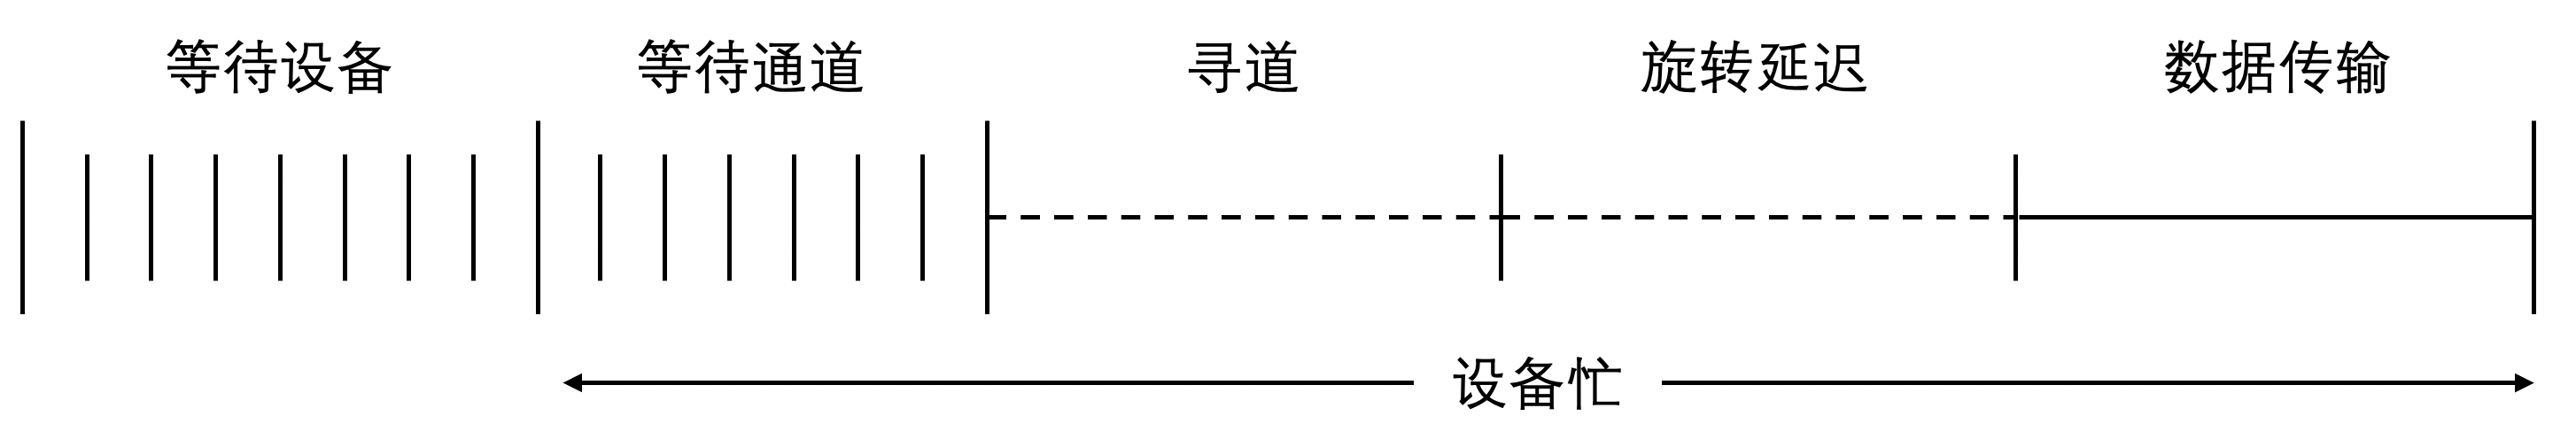
\includegraphics[width=0.8\textwidth]{img/4.4.1.2}
	\end{figure}

	磁盘存取时间 $T_a$ 是磁盘完成数据读写所需要的时间,是寻道时间、旋转延迟、传送时间的总和$$T_a = T_s + \frac{1}{2r} + \frac{b}{rN}$$
	\begin{itemize}
		\item $T_s$ 表示寻道时间
		\item $r$ 表示磁盘旋转的角速度,$1/(2r)$ 表示平均旋转等待时间
		\item $b$ 表示读写的数据字节数,$N$ 表示每个磁道道字节数,$b/(rN)$ 表示平均传输时间
	\end{itemize}

	\subsection{磁盘的驱动调度}
	磁盘可能同时接收到若干 I/O请求,如果随机选择并响应 I/O 请求,可能得到最坏的性能

	驱动调度是指系统采用一种调度策略,尽可能按最佳次序执行要求访问磁盘的多个 I/O 请求
	\begin{itemize}
		\item 能减少为若干 I/O 请求服务所需要消耗的总时间
		\item 驱动调度策略包括移臂调度和旋转调度
	\end{itemize}

	\subsection{旋转调度}
	目的:使得旋转延迟的总时间最少

	\subsubsection{循环排序}
	通过优化 I/O 请求排序,在最少旋转圈数内完成位于同一柱面的访问请求

	旋转位置测定硬件和多磁头同时读写技术有利于提高旋转调度的效率

	\subsubsection{优化分布}
	通过信息在存储空间的排列方式来减少旋转延迟

	如果沿着磁道按序对扇区编号,可能由于磁盘转速太快,造成处理当前扇区的数据时,下一个扇区已经跳过,需要再转一圈才能继续读数据
	\begin{itemize}
		\item 因此,对扇区编号时会间隔编号,例如交叉因子为 $2:1$ 表示相邻编号之间会间隔 1 个扇区,$3:1$ 表示会间隔 2 个扇区
	\end{itemize}

	按柱面而非盘面进行数据读写
	\begin{itemize}
		\item 连续记录数据时,先记录在同一柱面的不同磁道上, 然后再更换柱面,可以减少数据读写时的移臂操作
	\end{itemize}

	\textbf{例:}考虑 10 条逻辑记录 $A, B, \cdots, J$ 被存放于某旋转型设备上,假设每道存放 10 个物理块,旋转速度为一周 20 ms,处理程序读出每块后需要花费 4 ms 进行处理
	\begin{figure}[H]
		\centering
		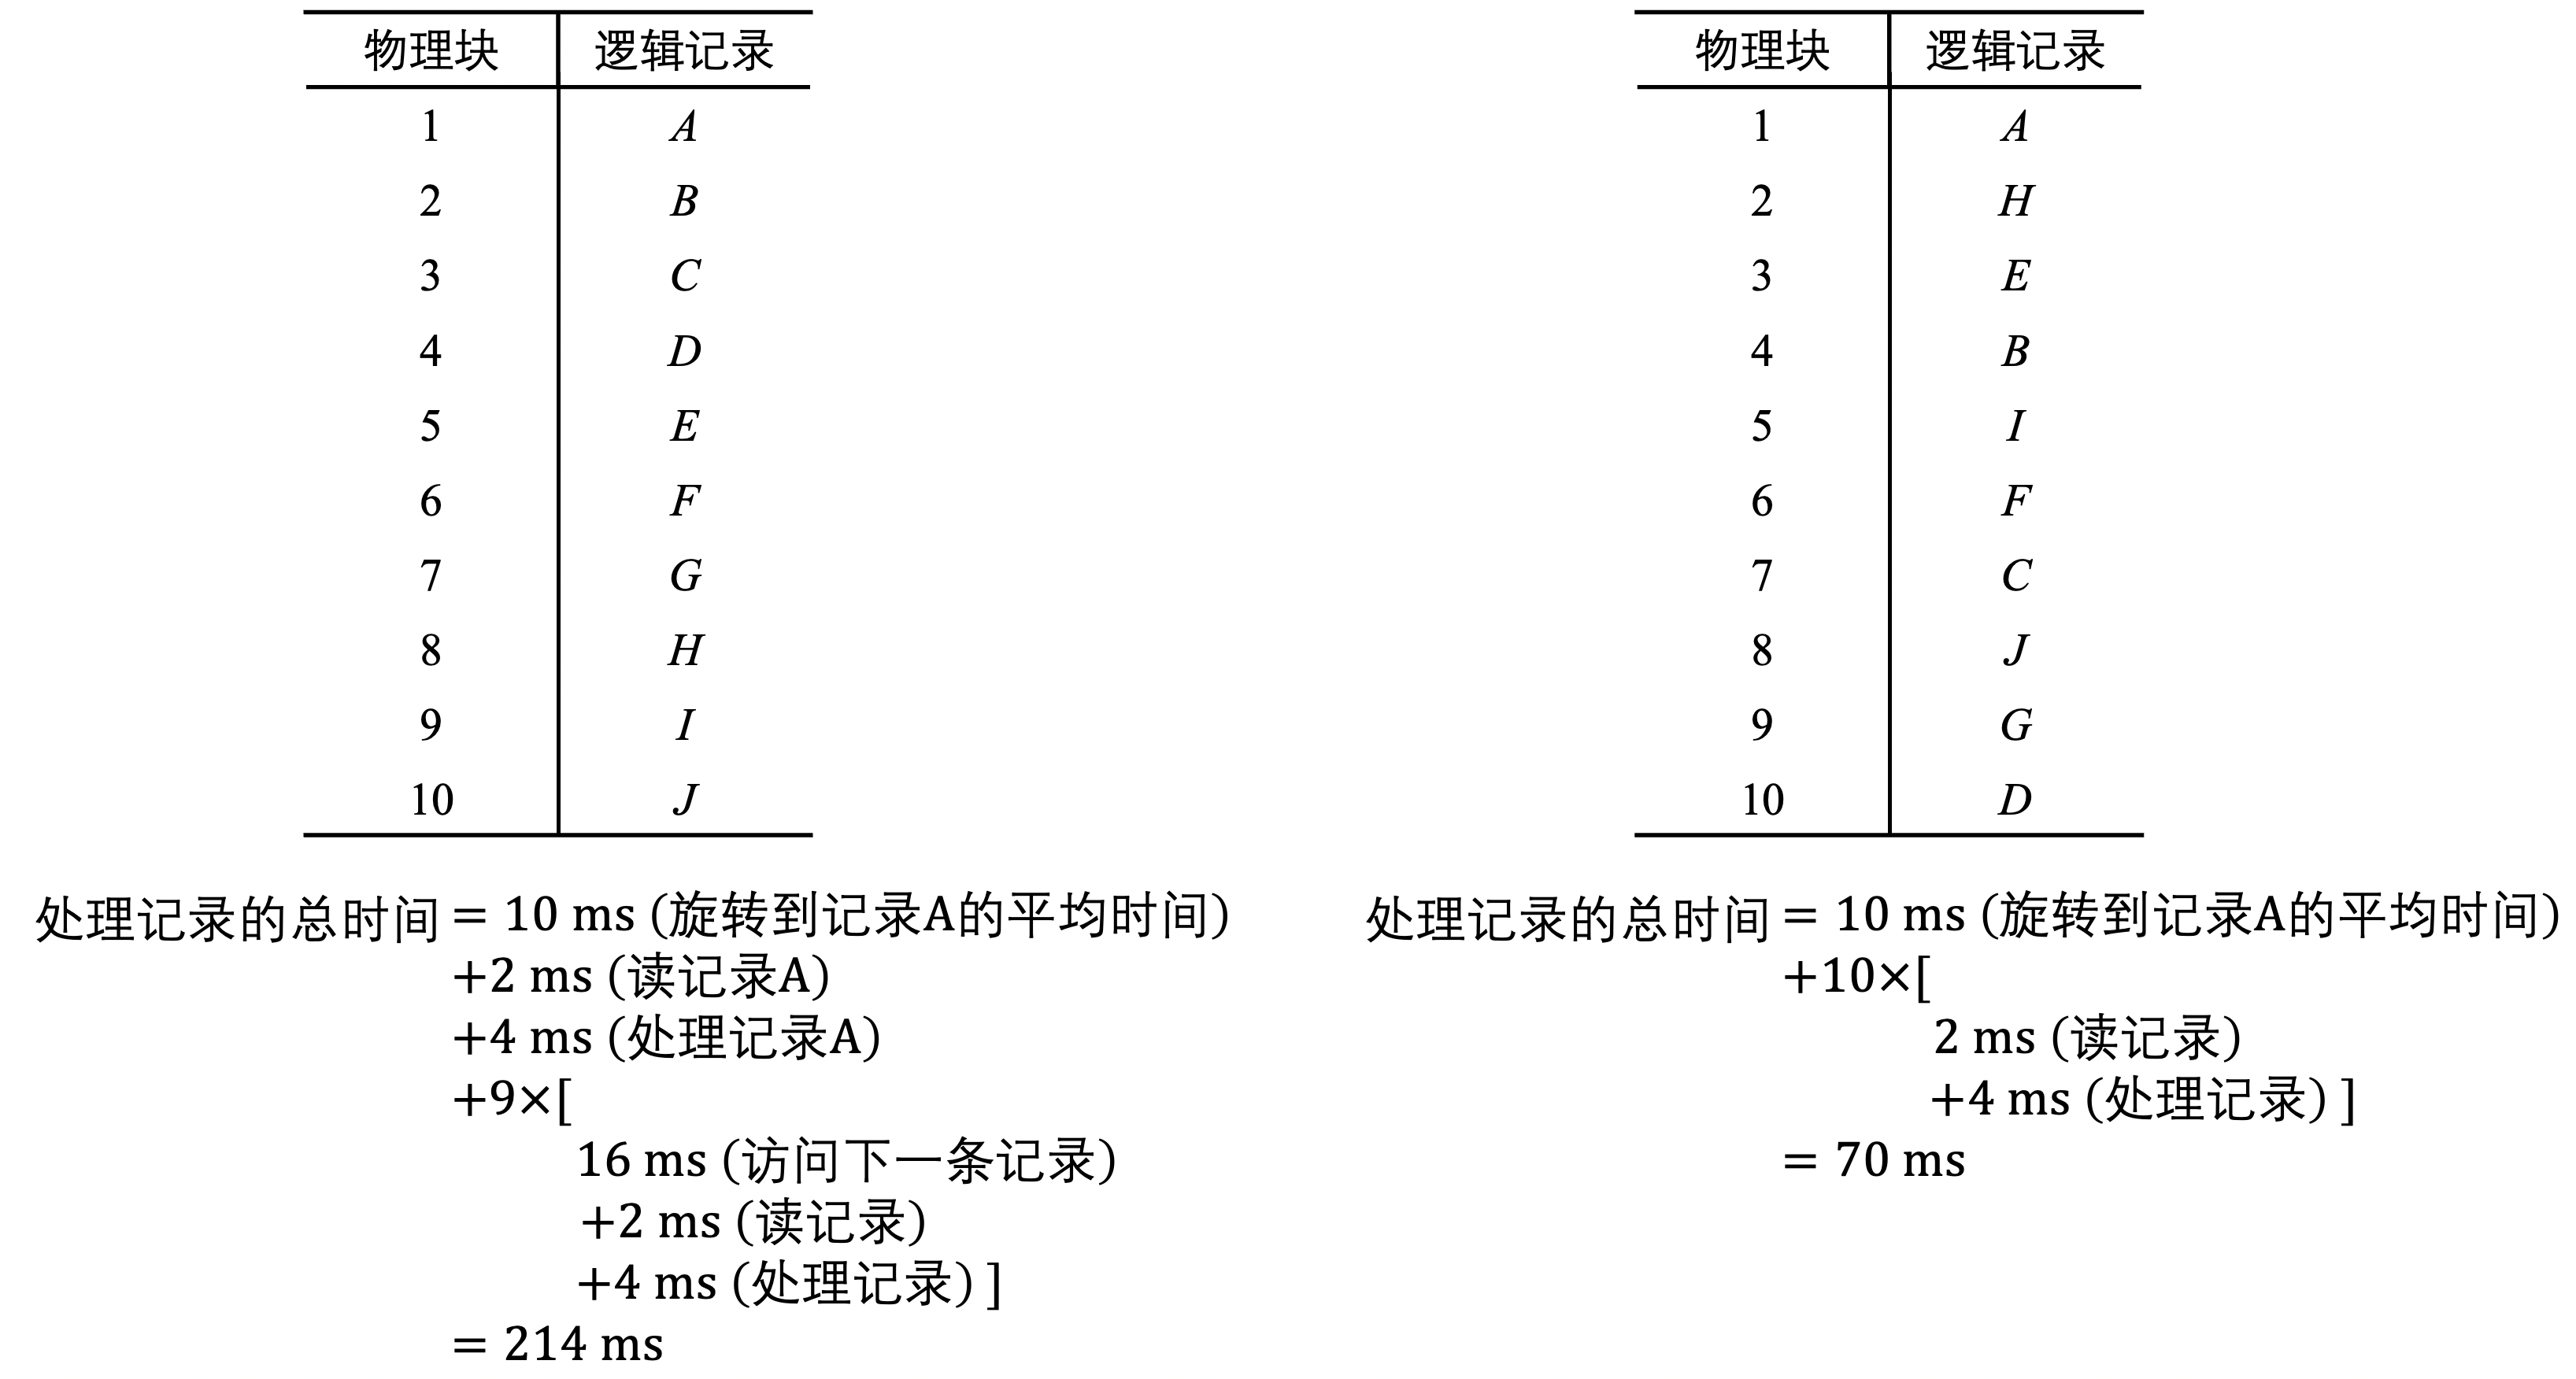
\includegraphics[width=0.9\textwidth]{img/4.4.3.2}
	\end{figure}

	对于优化前而言,读出并处理记录 $A$ 之后将旋转到记录 $D$ 的开始处,为了读出记录 $B$,必须再转一周;对于优化后而言,当读出记录 $A$ 并处理结束后,恰巧旋转至记录 $B$ 的位置,就可以立即读出记录 $B$ 并处理

	\subsection{移臂调度}

	\subsubsection{先来先服务FCFS}
	\begin{itemize}
		\item 移臂距离大,性能不好,移动臂是随机移动,寻道性能较差
		\item 按顺序处理请求,对所有进程公平
	\end{itemize}
	\begin{figure}[H]
		\centering
		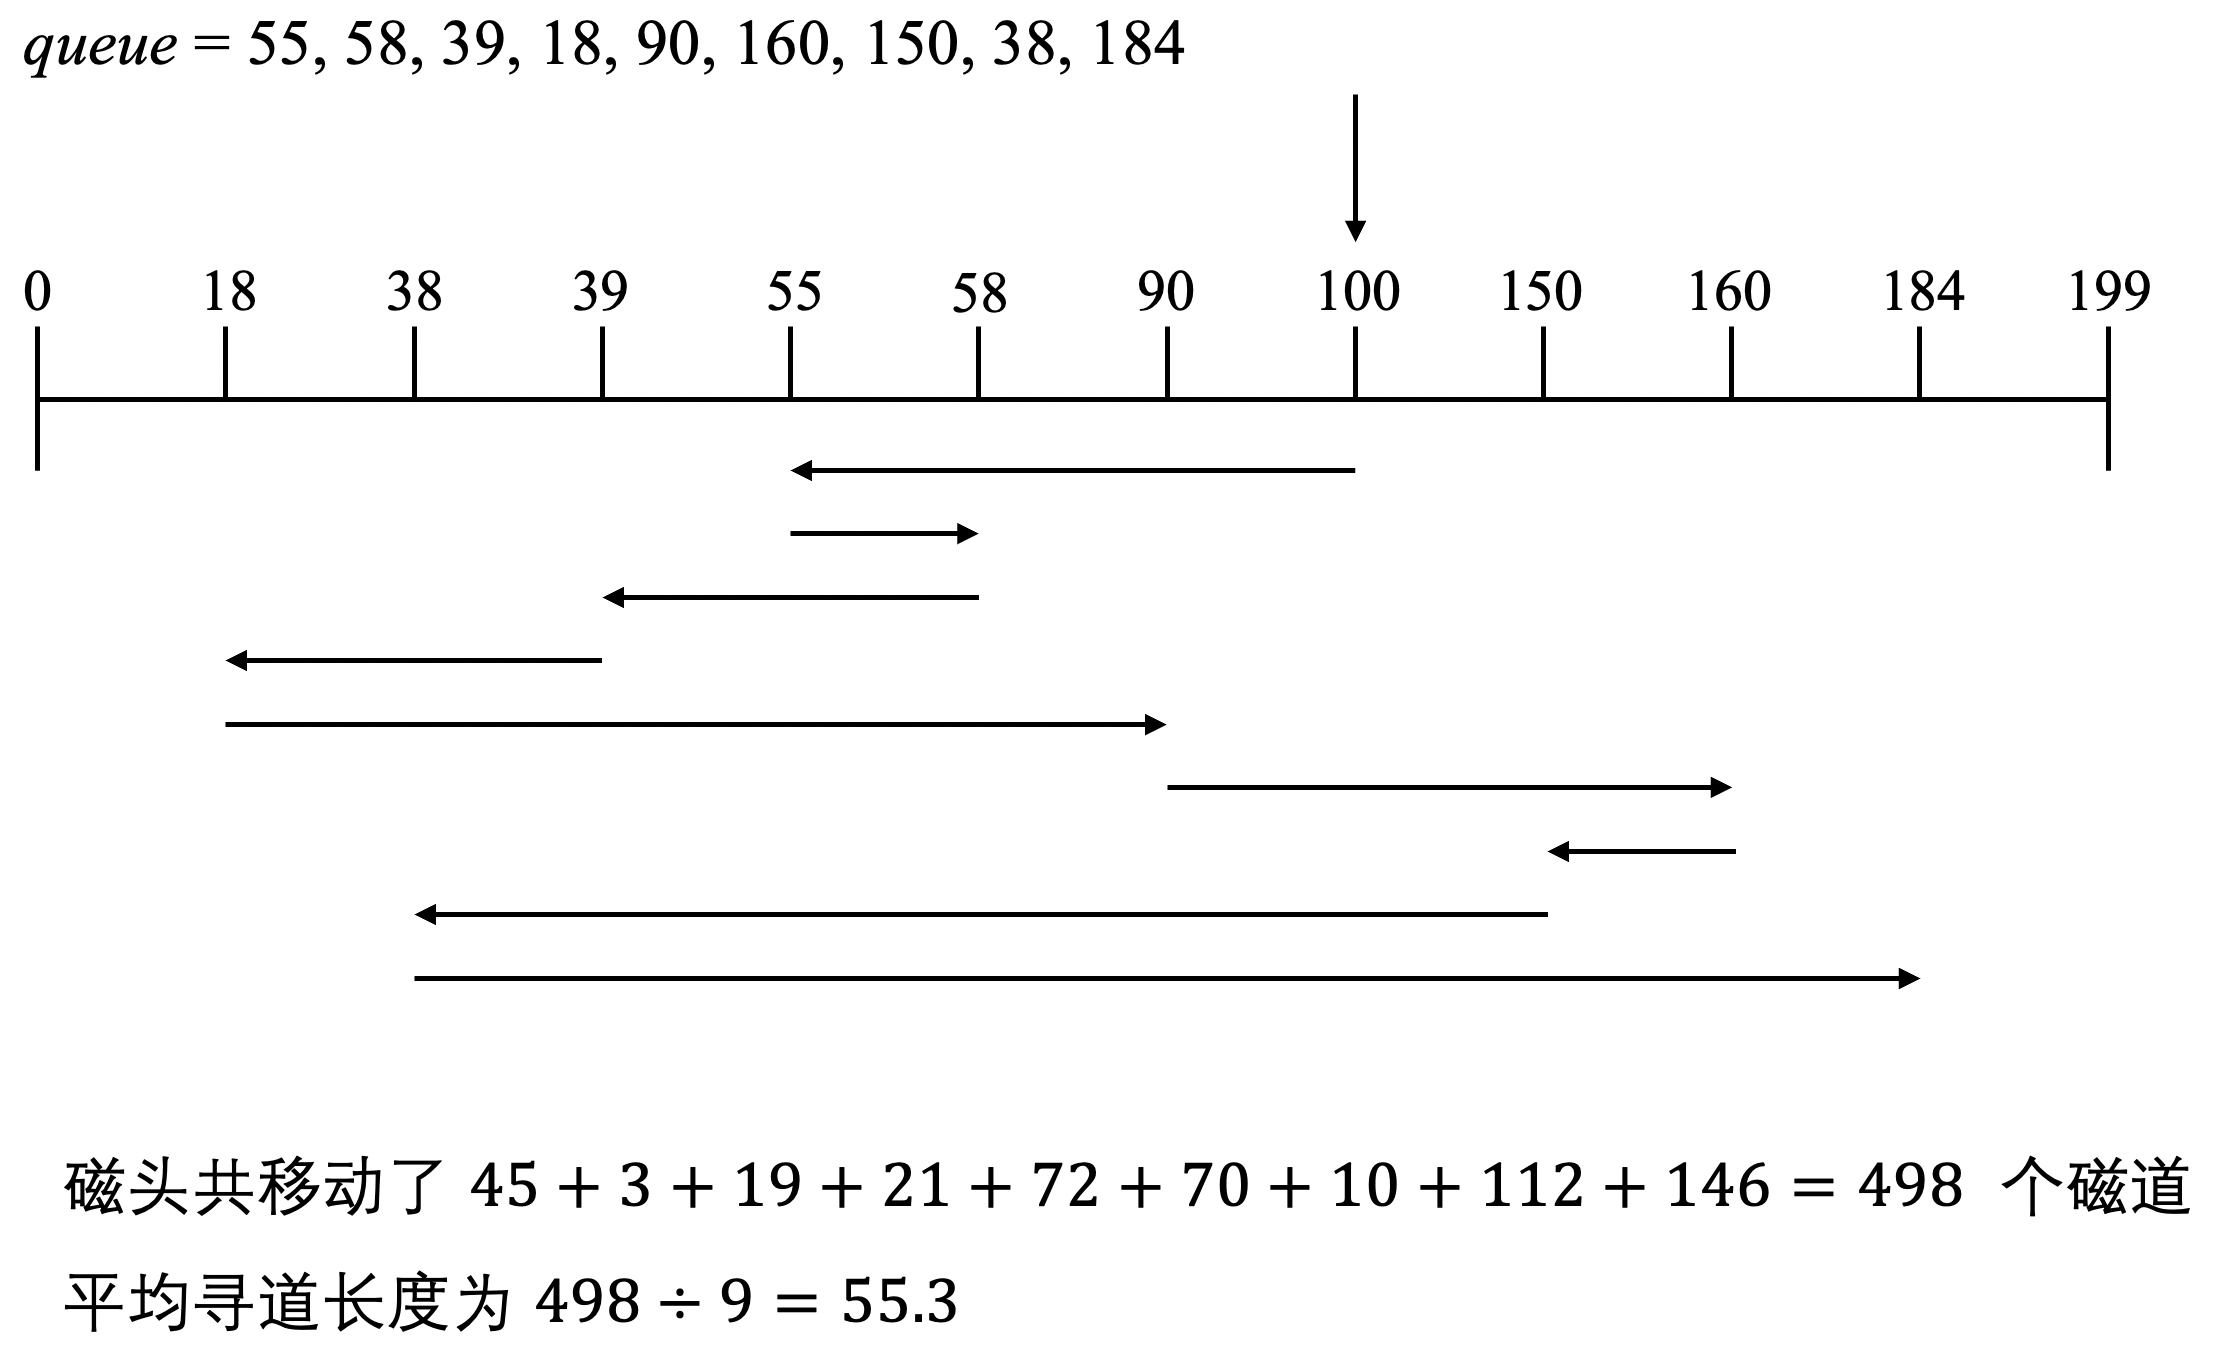
\includegraphics[width=0.9\textwidth]{img/FCFS disk}
	\end{figure}

	\subsubsection{最短查找时间优先SSTF}
	\begin{itemize}
		\item 先执行查找时间最短的请求,具有较好的寻道性能
		\item 存在“饥饿”现象:距离比较远的很难被满足
		\item 总是选择最小寻道时间并不能保证平均寻道时间最小,但是它的性能比 FCFS 更好
	\end{itemize}
	\begin{figure}[H]
		\centering
		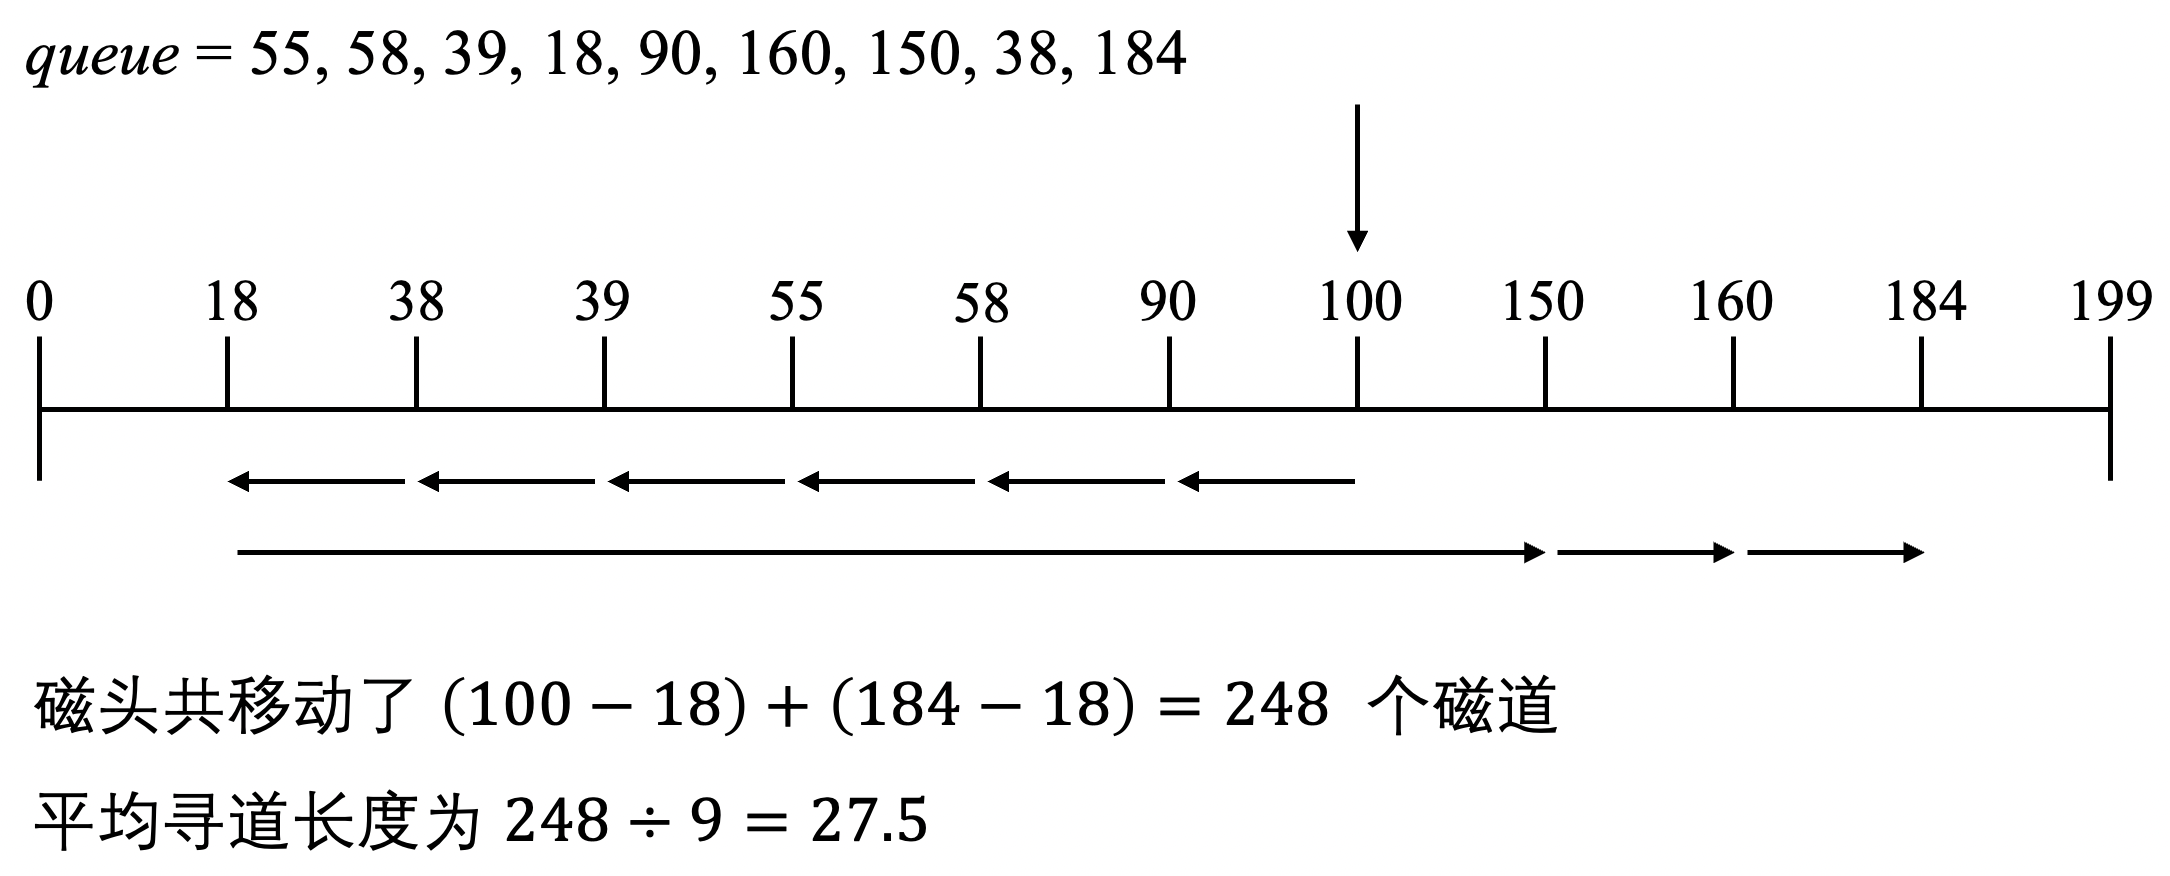
\includegraphics[width=0.9\textwidth]{img/SSTF}
	\end{figure}

	\subsubsection{扫描算法SCAN}
	\begin{itemize}
		\item 移动臂每次向一个方向移动,遇到最近的 I/O 请求便进行处理,到达最后一个柱面后再向相反方向移动
		\item 对最近扫描所跨越区域的请求响应较慢
	\end{itemize}
	\begin{figure}[H]
		\centering
		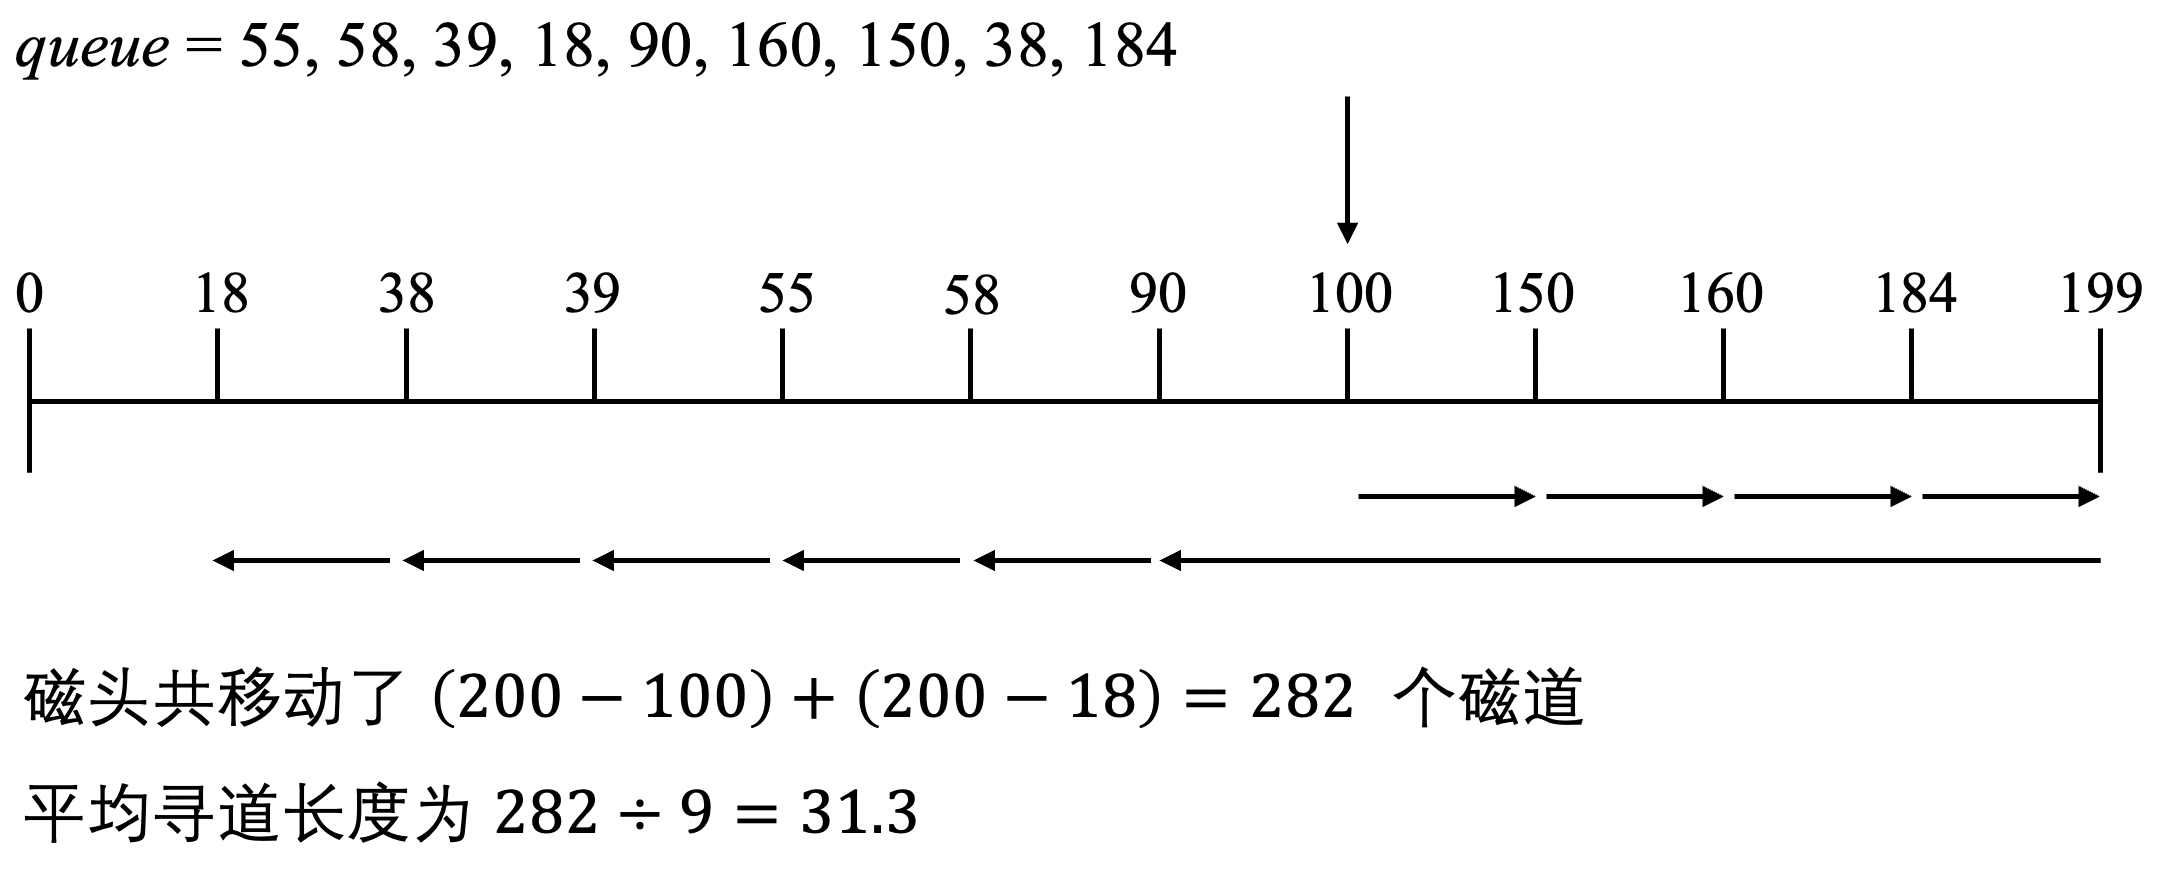
\includegraphics[width=0.9\textwidth]{img/SCAN}
	\end{figure}

	\subsubsection{LOOK算法}
	\begin{itemize}
		\item 无请求时移动臂停止不动,有请求时按电梯规律移动
		\item 每次选择沿移动臂的移动方向最近的柱面
		\item 如果当前移动方向上没有但相反方向有请求时,改变移动方向
	\end{itemize}
	\begin{figure}[H]
		\centering
		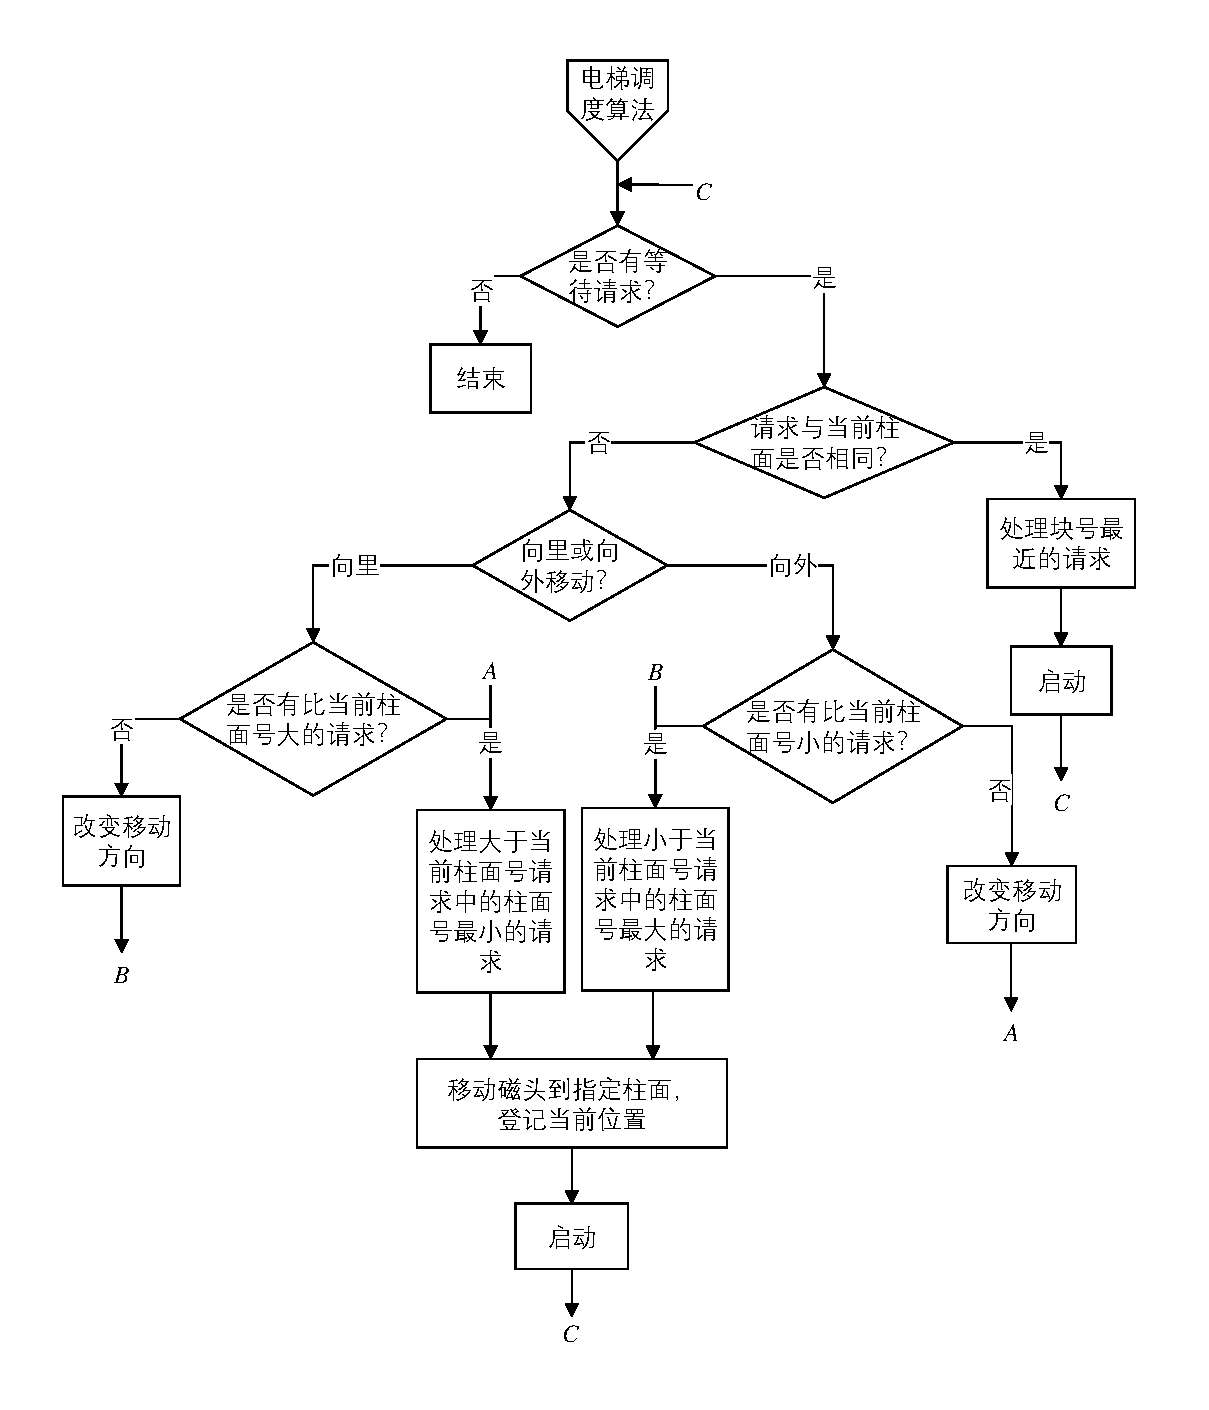
\includegraphics[width=0.8\textwidth]{img/LOOK.pdf}
	\end{figure}
	\begin{figure}[H]
		\centering
		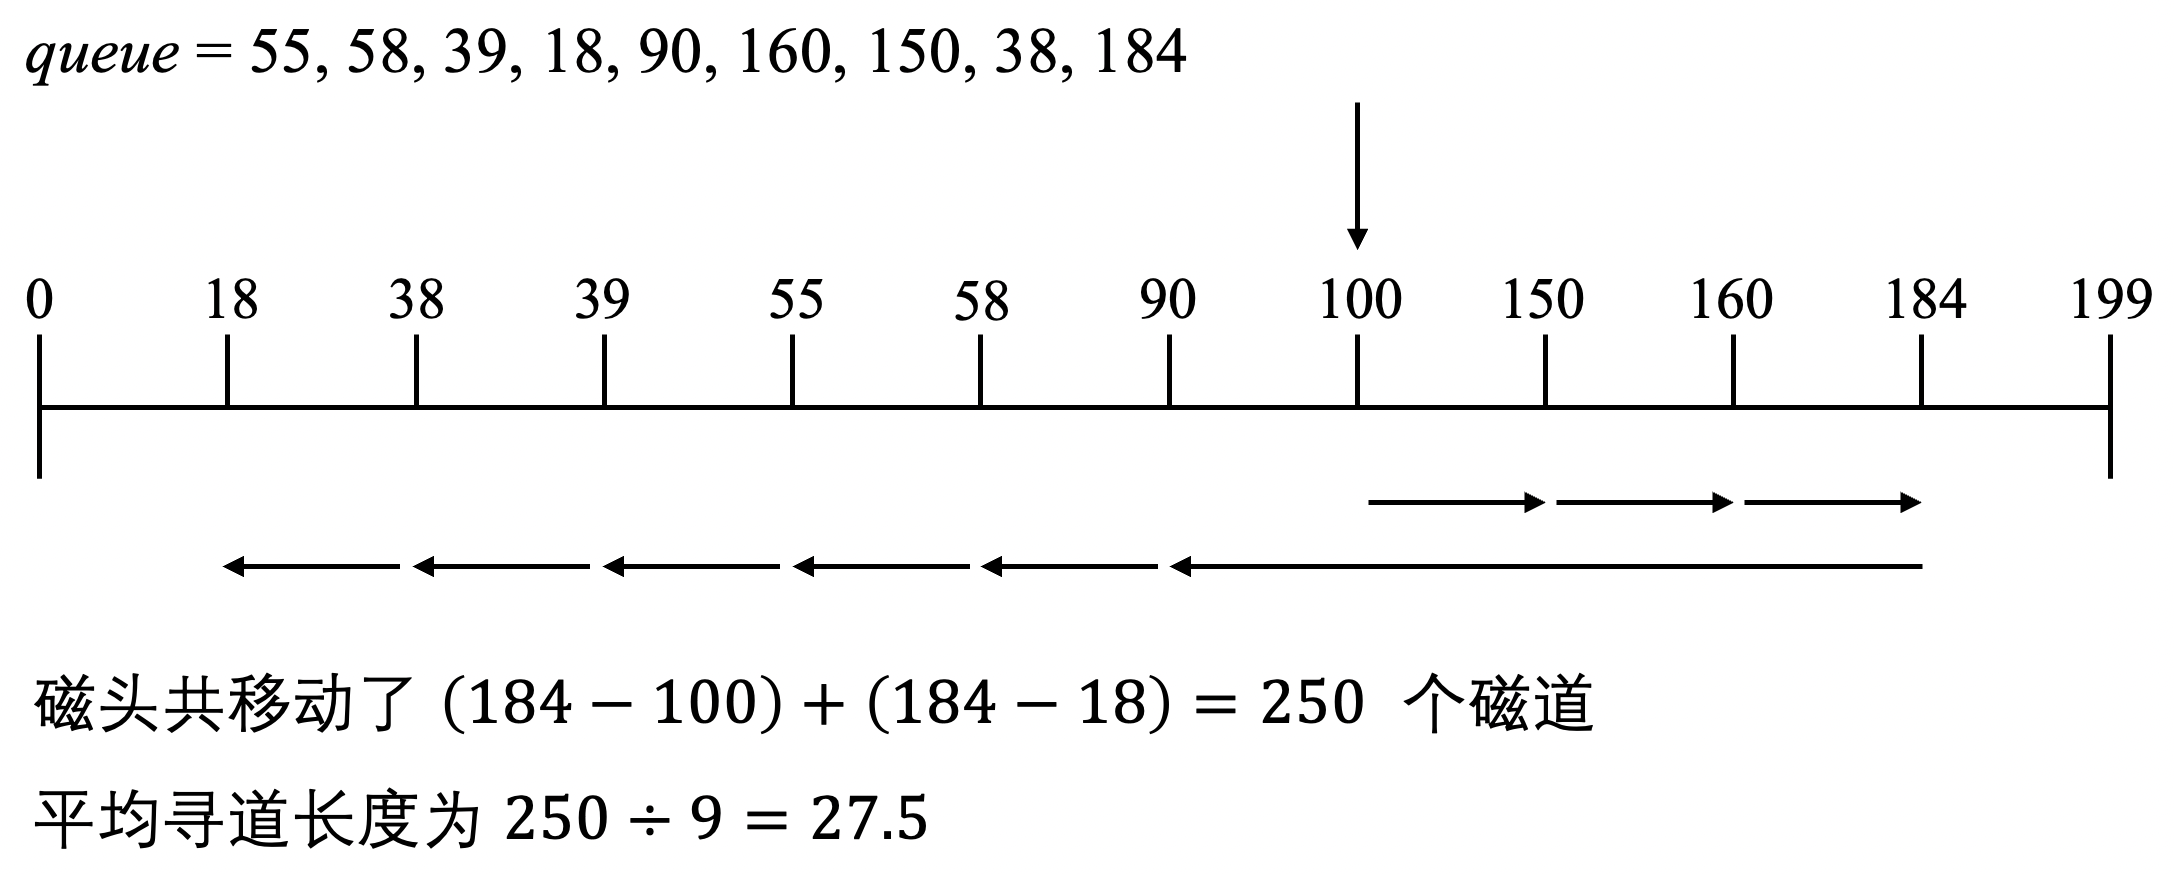
\includegraphics[width=0.9\textwidth]{img/LOOK.png}
	\end{figure}

	\subsubsection{循环扫描C-SCAN}
	\begin{itemize}
		\item 把扫描限定在一个方向
		\item 当访问到沿某个方向的最后一个磁道时,磁头臂返回到磁盘相反方向磁道的末端,并再次开始扫描
	\end{itemize}
	\begin{figure}[H]
		\centering
		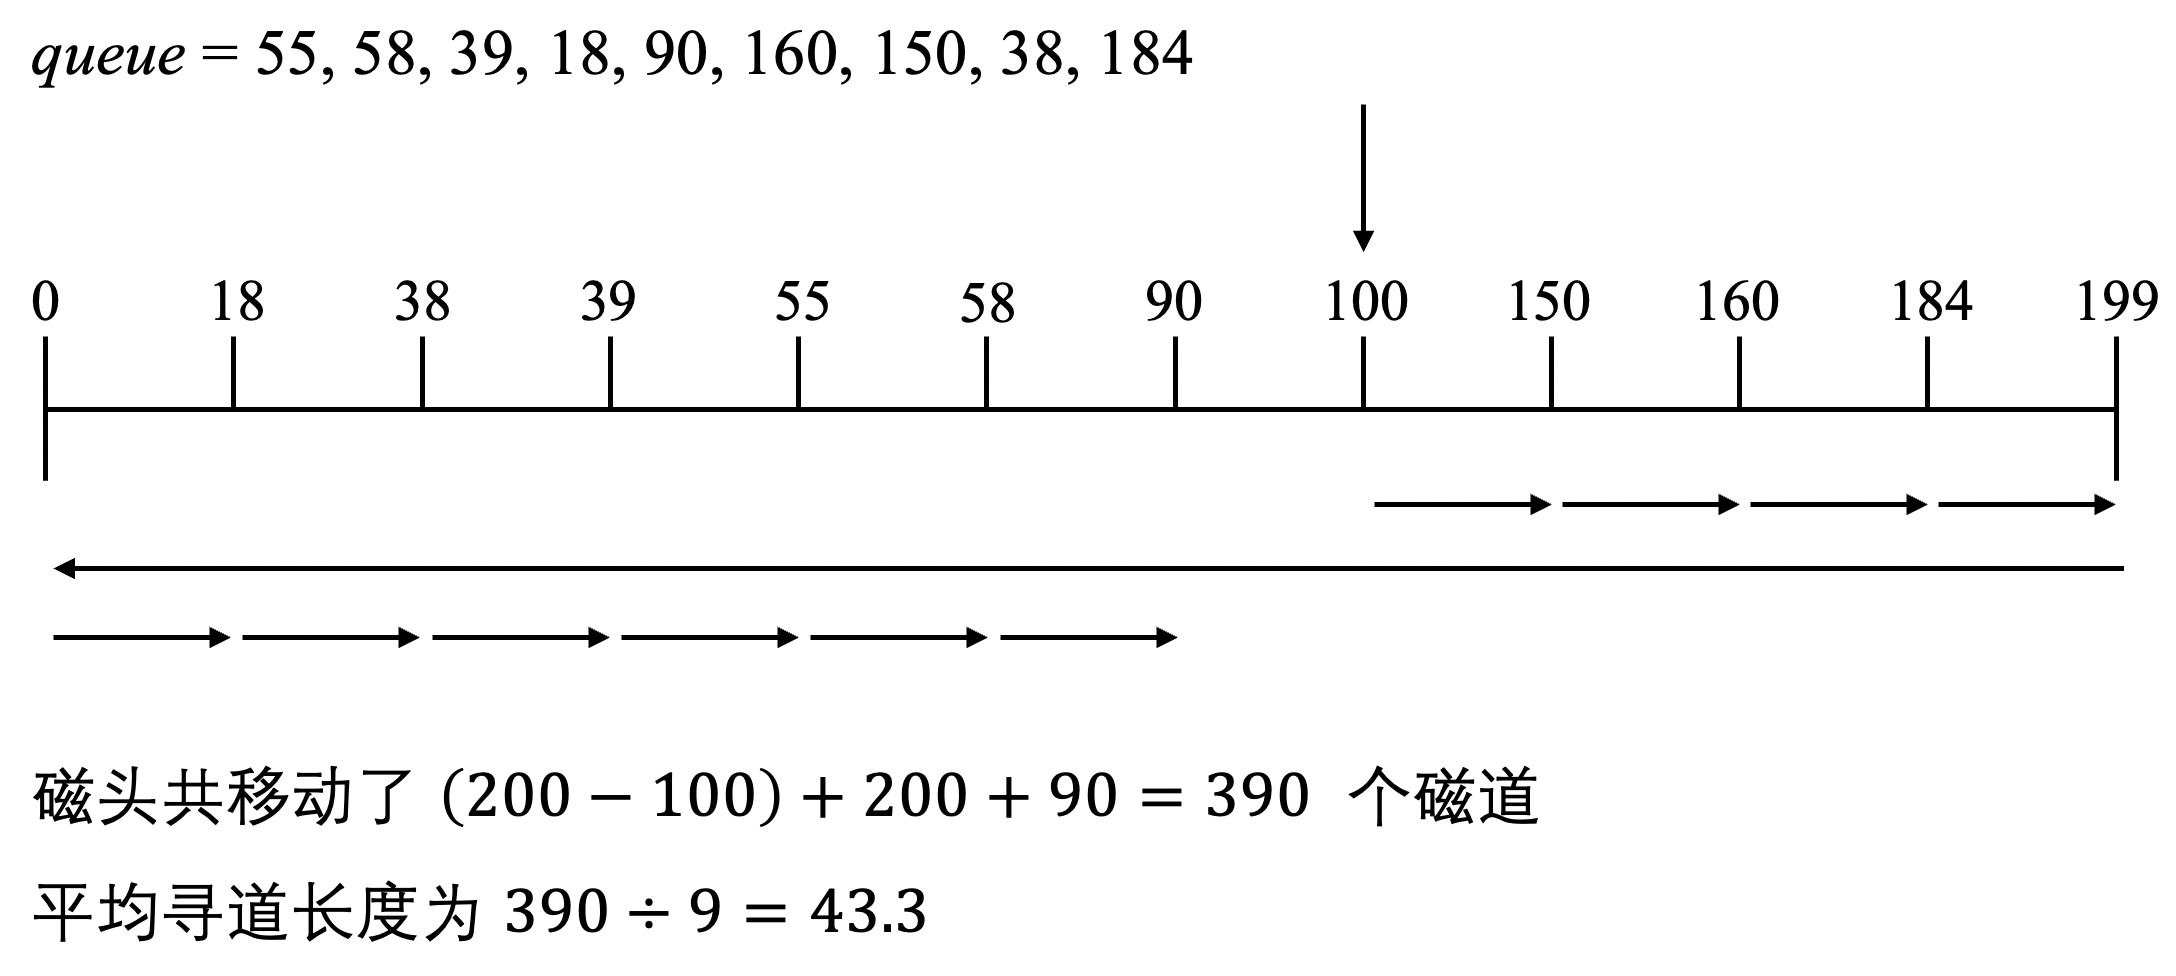
\includegraphics[width=0.9\textwidth]{img/C-SCAN}
	\end{figure}

	\subsubsection{C-LOOK算法}
	\begin{itemize}
		\item 磁头从初始请求开始到另一个方向的最后一个请求,并为中间的所有请求提供服务
		\item 磁头在一端完成最后一个请求后向另一个方向跳跃,并继续向剩余的请求前进,以与先前相同的方向完成它们
	\end{itemize}
	\begin{figure}[H]
		\centering
		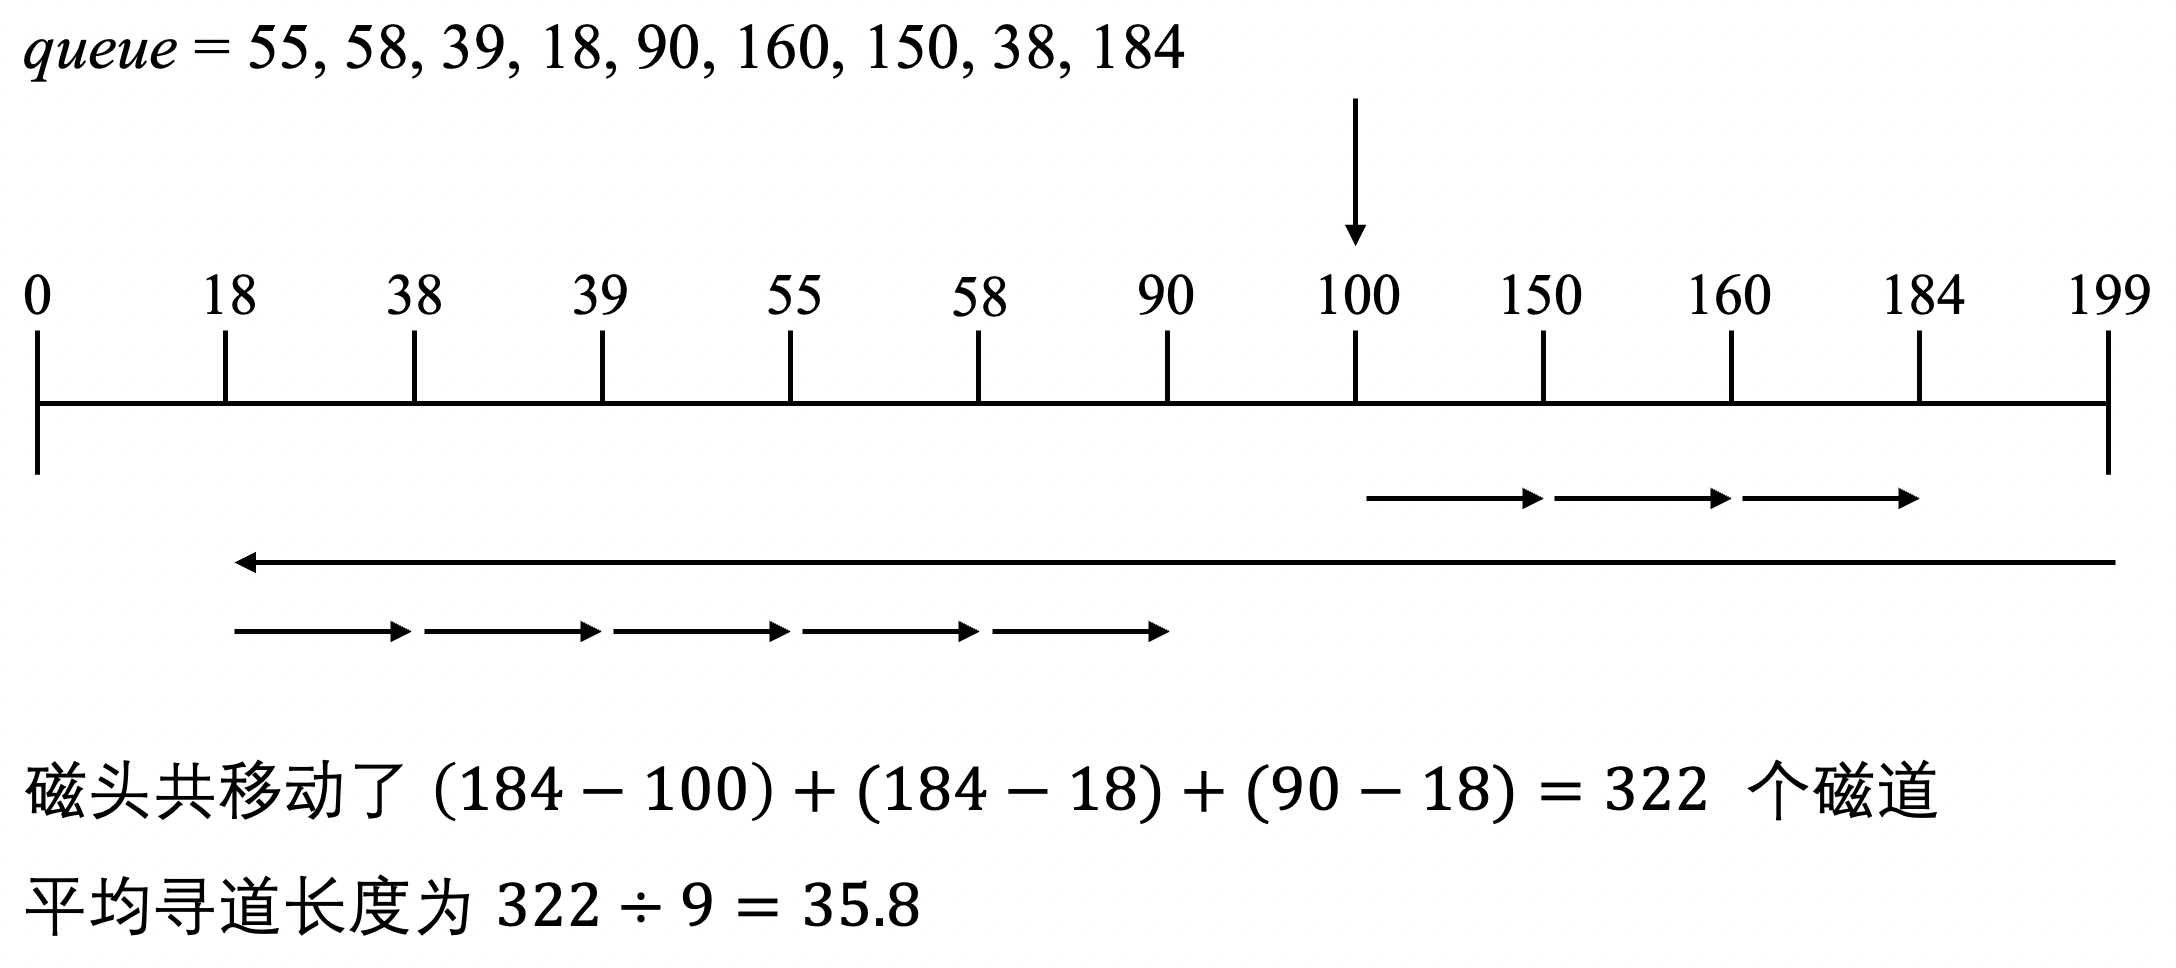
\includegraphics[width=0.9\textwidth]{img/C-LOOK}
	\end{figure}

	\subsection{提高磁盘I/O速度的办法}
	\textbf{提前读:}按照顺序访问时,可以读当前磁盘块时,提前把下一个磁盘块的数据也读入磁盘缓冲区

	\textbf{延迟写:}由于缓冲区的数据不久以后还会再次被进程访问,因此不立即将缓冲区中的数据写回盘,而是挂载空闲缓冲区队列队尾,直到移动到空闲缓冲区队首时在写回

	\textbf{虚拟盘:}用内存空间仿真磁盘,又叫 RAM 盘,相应的操作在内存中执行而不是硬盘中,比如浏览器缓存等

	\subsection{磁盘循环冗余阵列}

	\subsubsection{RAID\ 0}
	连续的数据条带以轮转方式写到全部磁盘上,然后采用并行交叉存取,减少 I/O 请求排队时间,适用于大数据量的 I/O 请求

	并无冗余校验功能,可靠性较差
	\begin{figure}[H]
		\centering
		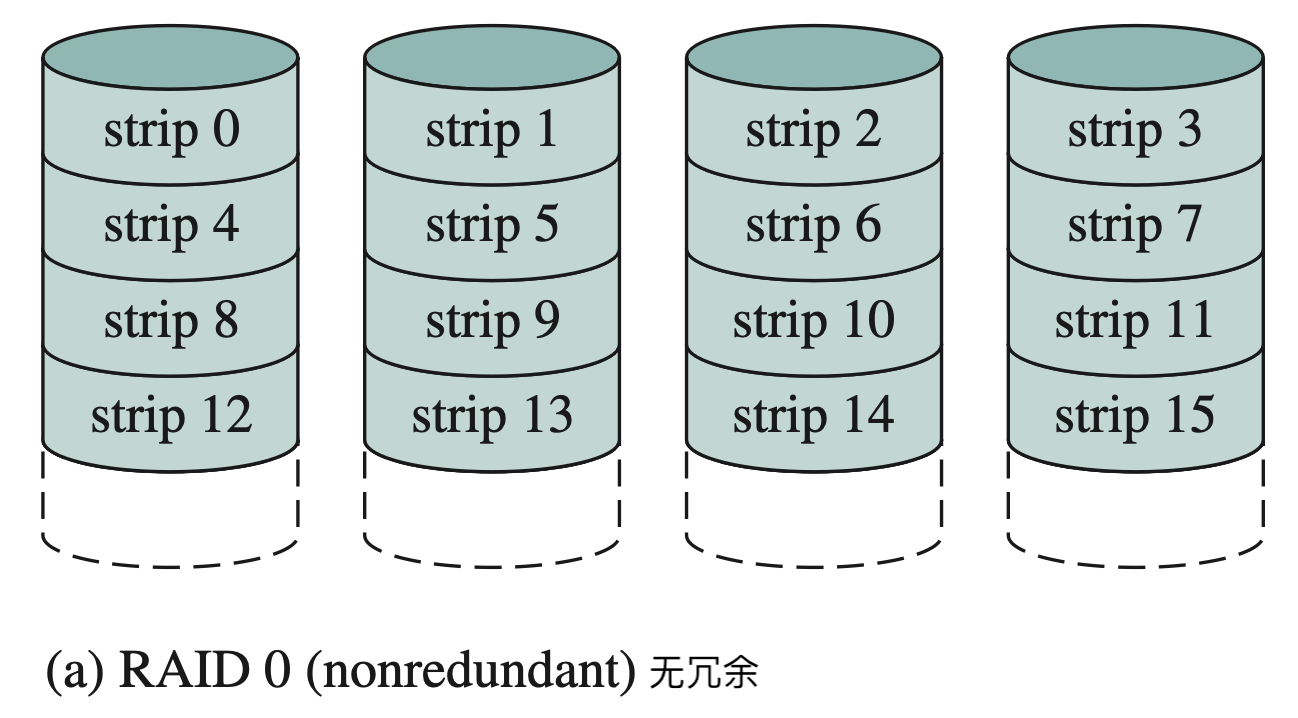
\includegraphics[width=0.4\textwidth]{img/RAID0}
	\end{figure}

	RAID\ 0 的数据映射
	\begin{figure}[H]
		\centering
		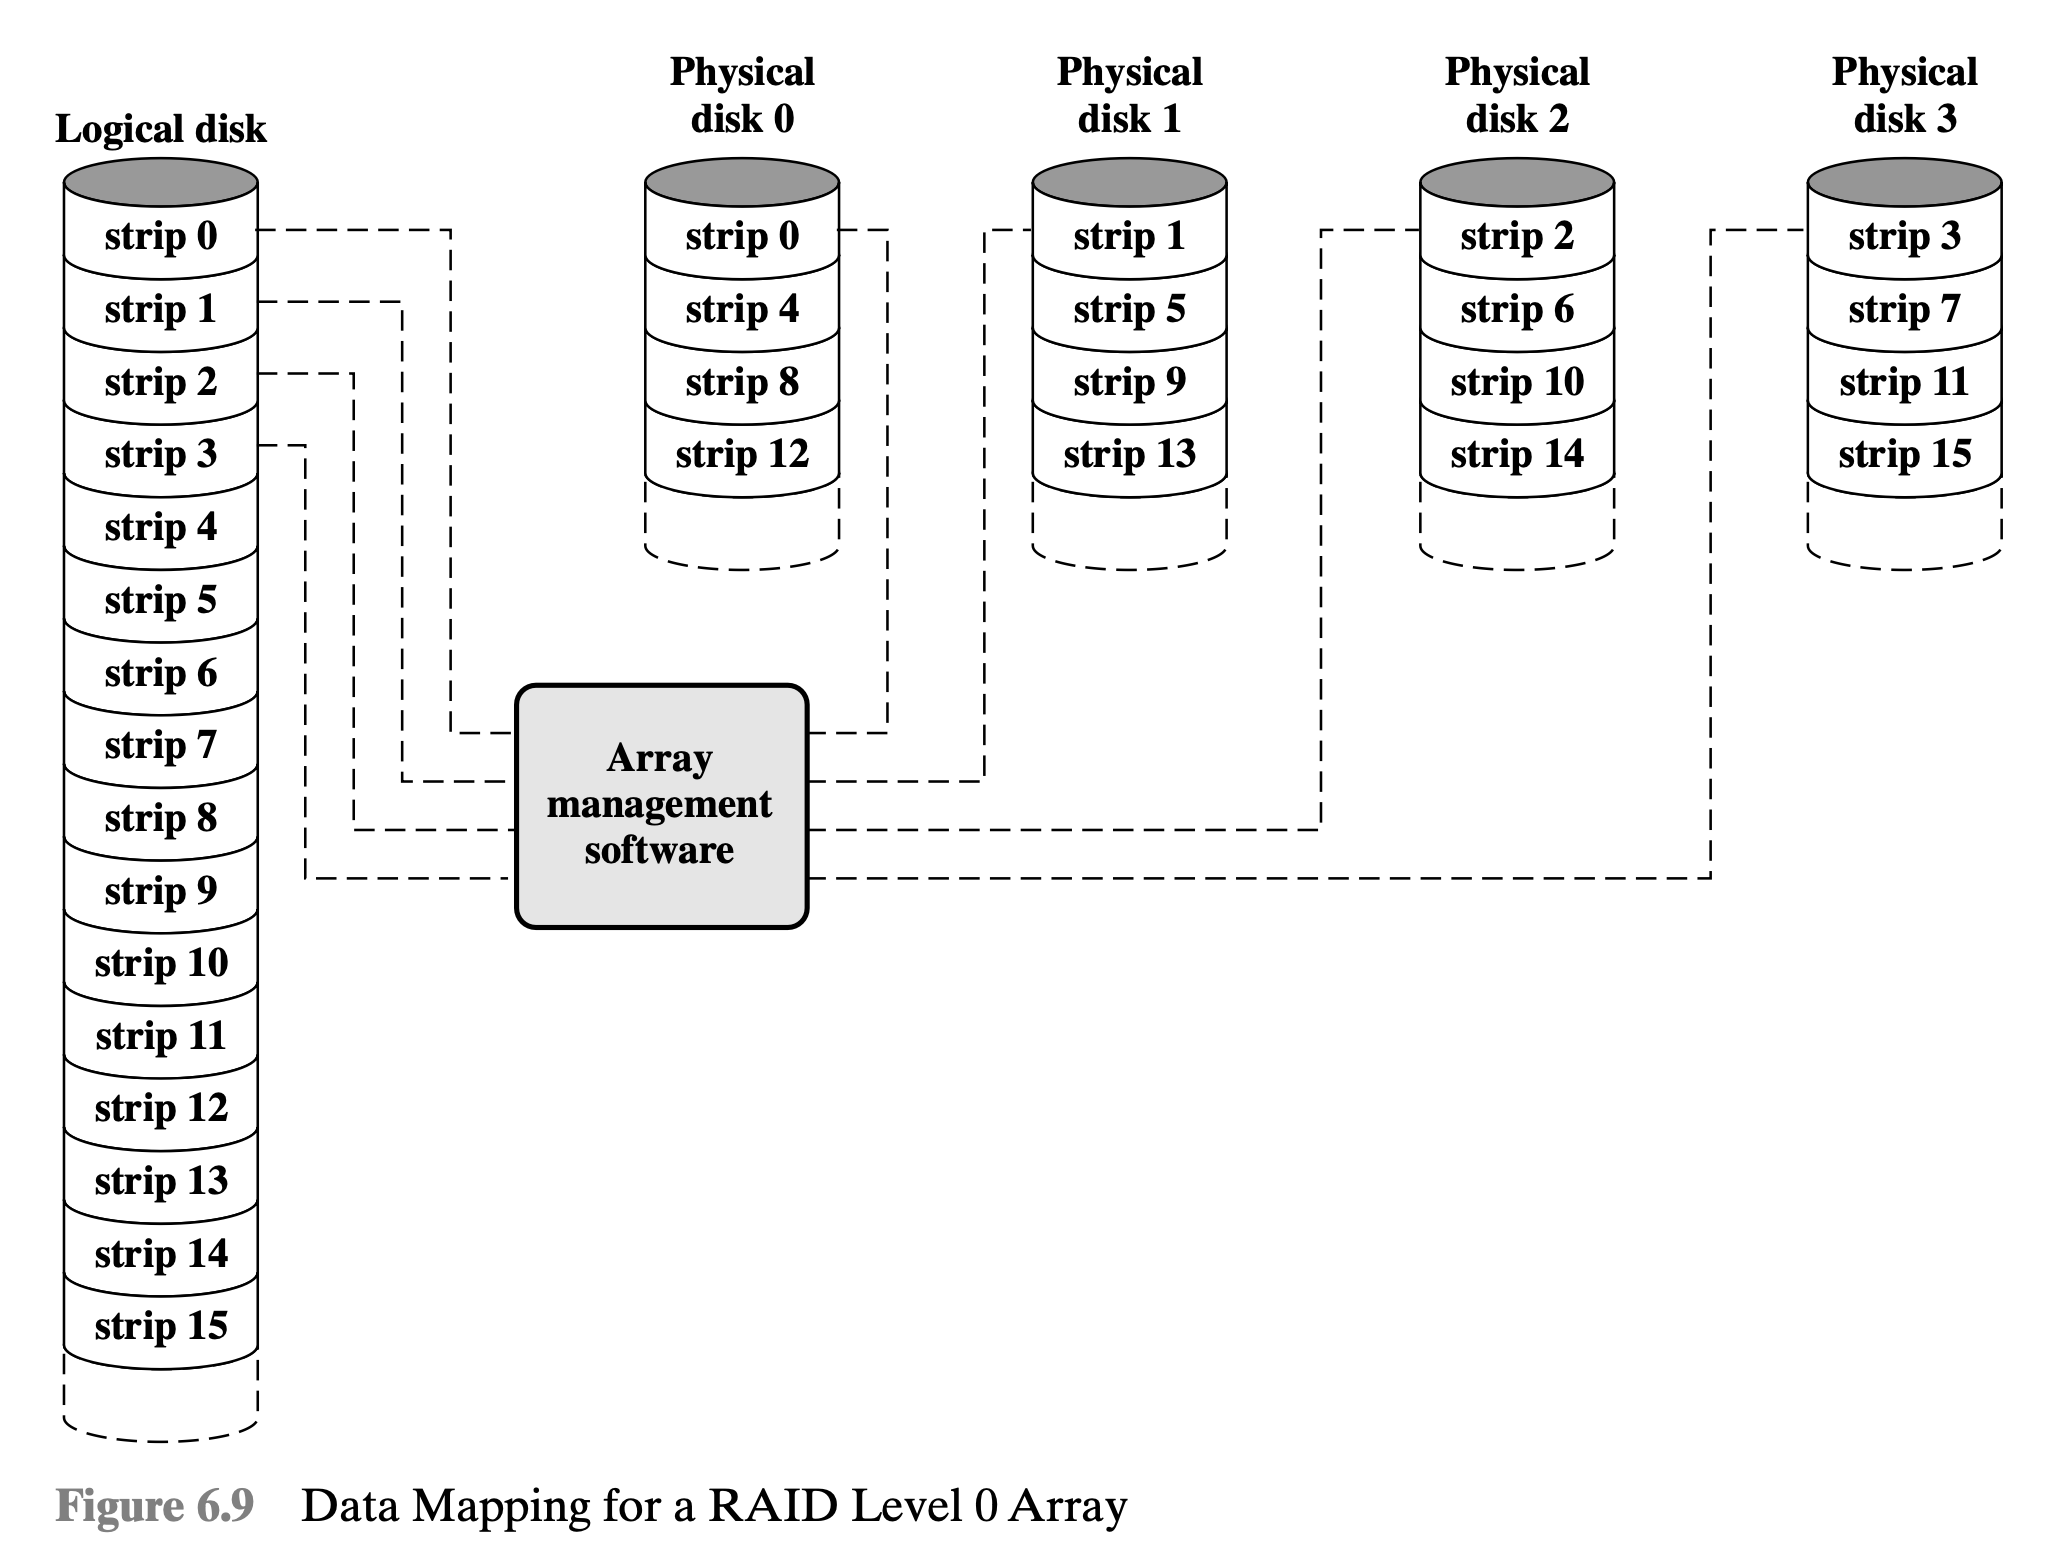
\includegraphics[width=0.6\textwidth]{img/RAID0-1}
	\end{figure}

	\subsubsection{RAID\ 1}
	采用镜像盘双份所有数据来提高容错性,读请求拥有最小寻道时间,写请求可并行完成

	缺点是容量下降一半,故成本很高
	\begin{figure}[H]
		\centering
		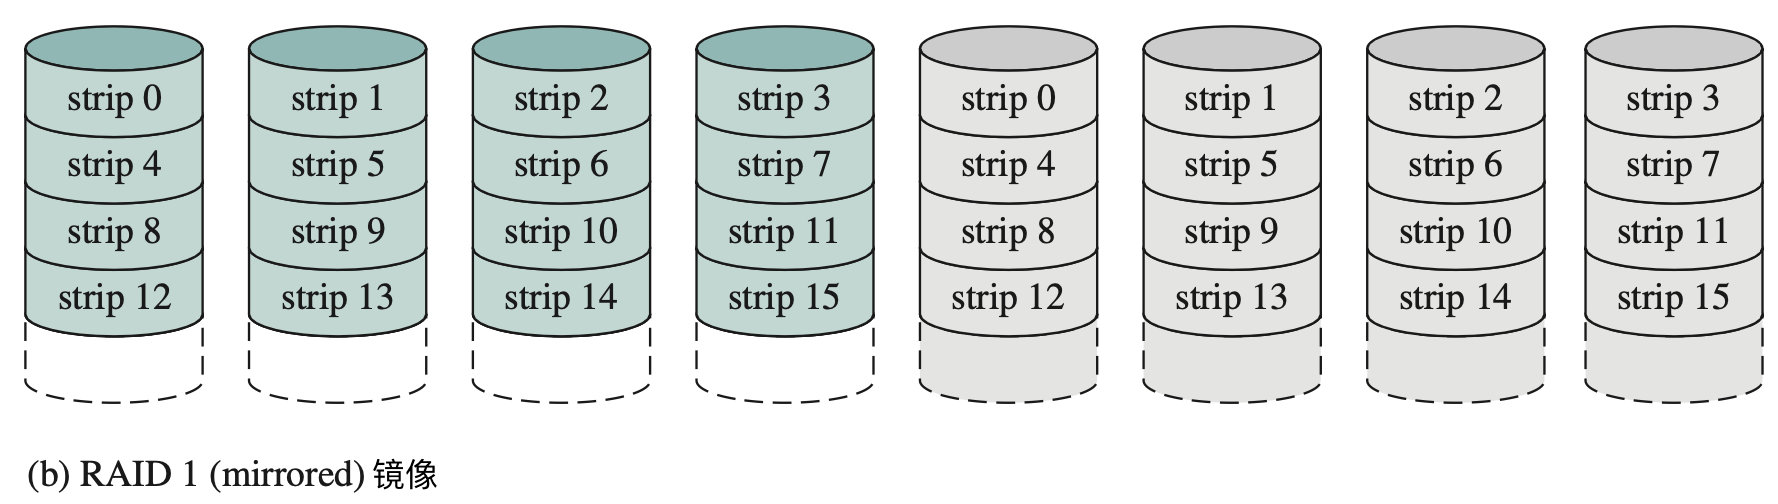
\includegraphics[width=0.8\textwidth]{img/RAID1}
	\end{figure}

	\subsubsection{RAID\ 2}
	采用数据字或字节交叉存放,并行存取获得高性能,使用海明校验码,适合大量顺序数据访问

	由于使用多个冗余盘,成本较高
	\begin{figure}[H]
		\centering
		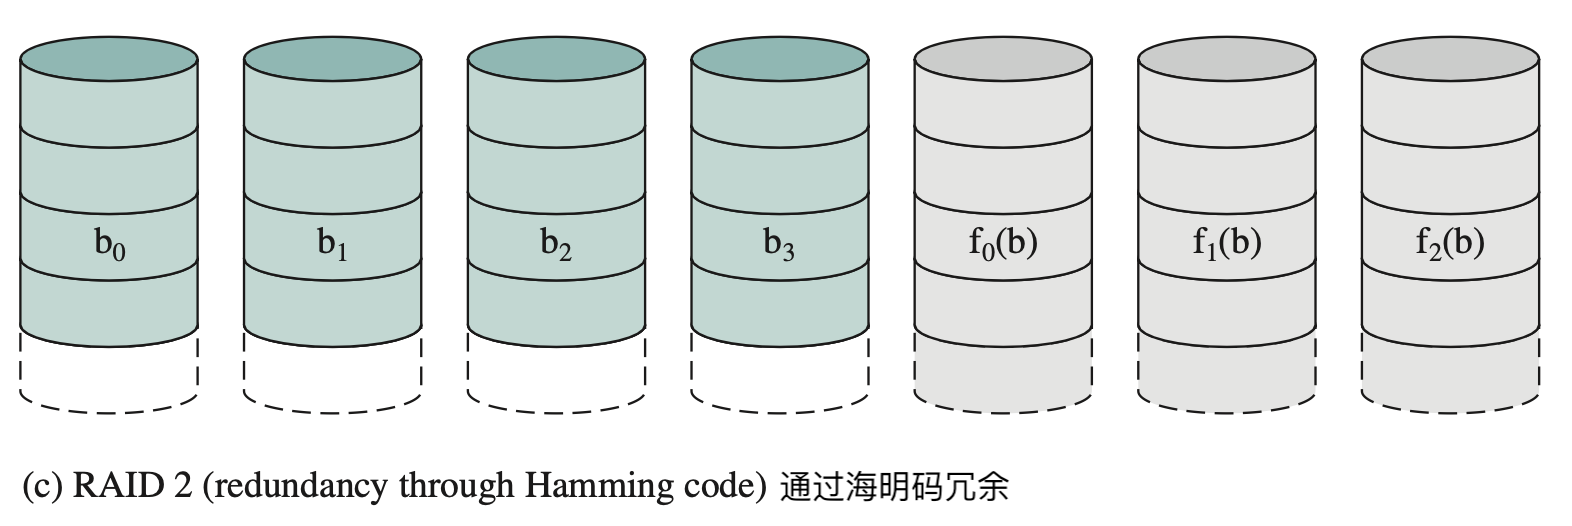
\includegraphics[width=0.8\textwidth]{img/RAID2}
	\end{figure}

	\subsubsection{RAID\ 3}
	RAID\ 3 是 RAID\ 2 的简化版本,差别是它仅用一只冗余盘,采用奇偶校验技术
	\begin{figure}[H]
		\centering
		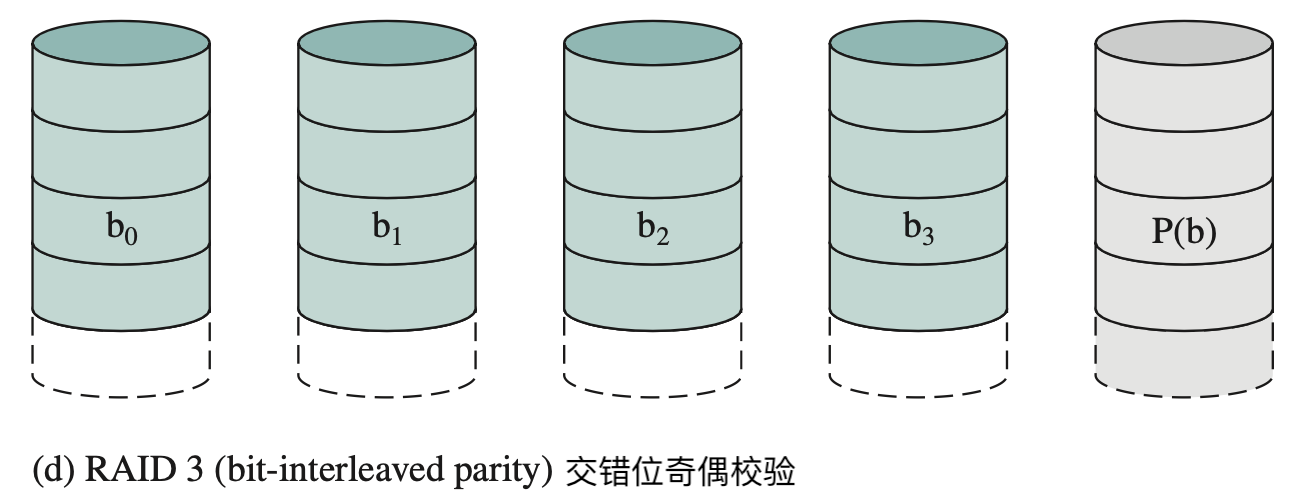
\includegraphics[width=0.8\textwidth]{img/RAID3}
	\end{figure}

	\subsubsection{RAID\ 4}
	采用独立存取磁盘阵列,数据条带交叉存放,访问请求可并行地获得满足,适合有较高 I/O 请求速度的应用场合。使用一只冗余盘存放奇偶校验码
	\begin{figure}[H]
		\centering
		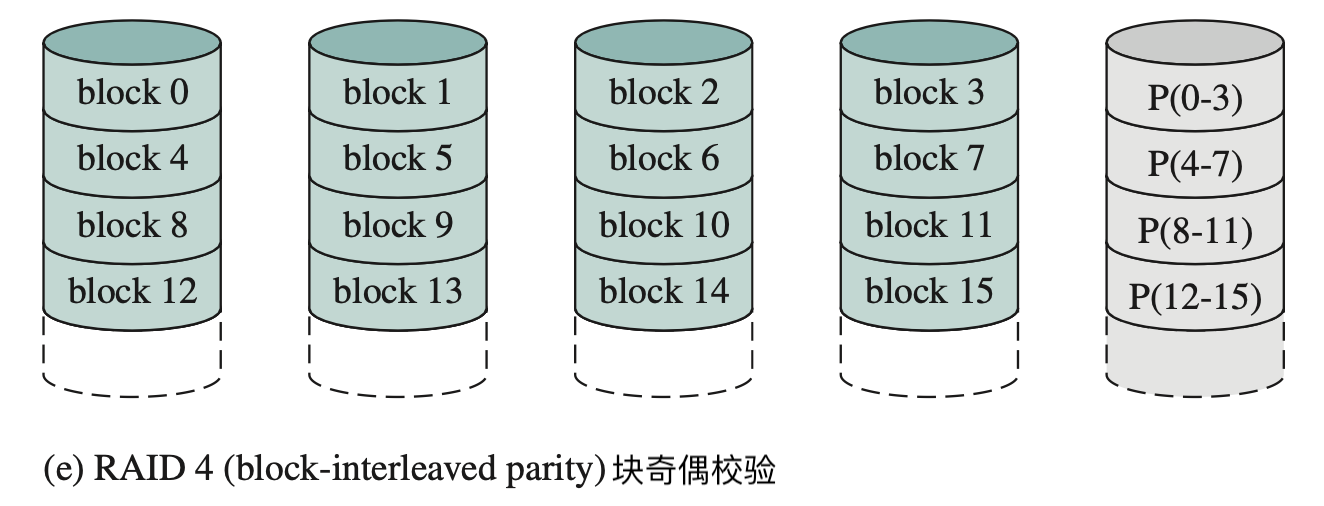
\includegraphics[width=0.8\textwidth]{img/RAID4}
	\end{figure}

	\subsubsection{RAID\ 5}
	RAID\ 5 与 RAID\ 4 的组织类似,但奇偶校验码循环分布在每个盘上,使得容错性更好
	\begin{figure}[H]
		\centering
		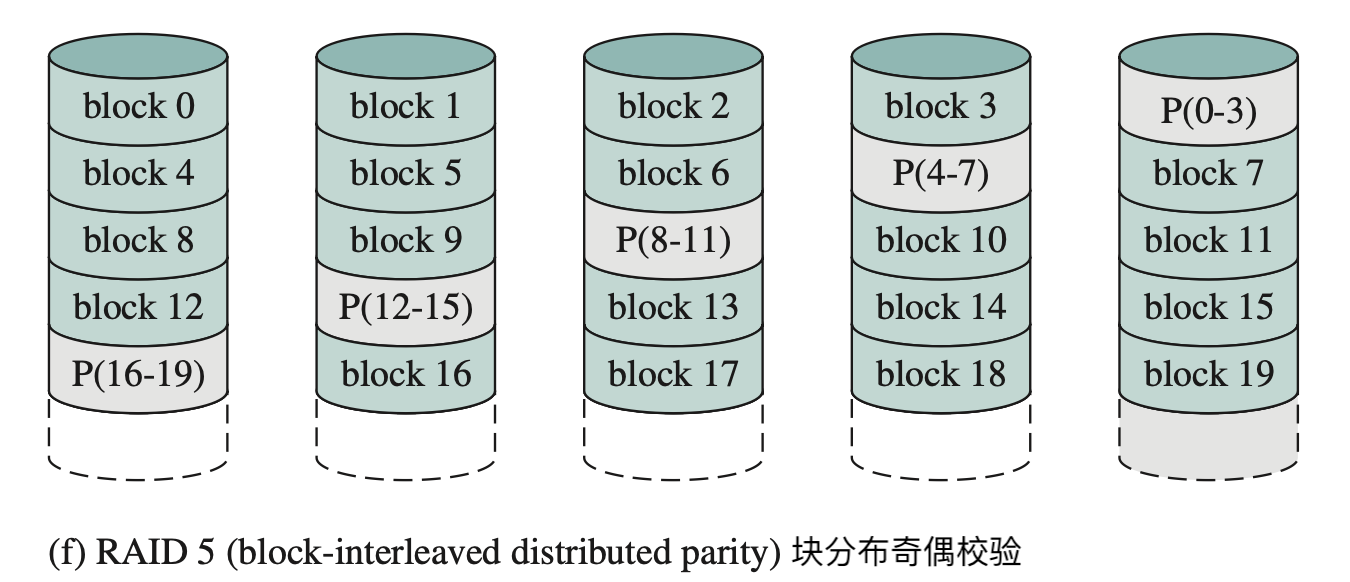
\includegraphics[width=0.8\textwidth]{img/RAID5}
	\end{figure}

	\subsubsection{RAID\ 6}
	采用双重冗余技术, $P$ 和 $Q$ 是两种不同的数据校验算法
	\begin{itemize}
		\item 其中一种是 RAID\ 4 和 RAID\ 5 所使用的异或计算
		\item 另一种是独立数据校验算法
	\end{itemize}
	即使有两个数据磁盘发生错误,也可重新生成数据
	\begin{figure}[H]
		\centering
		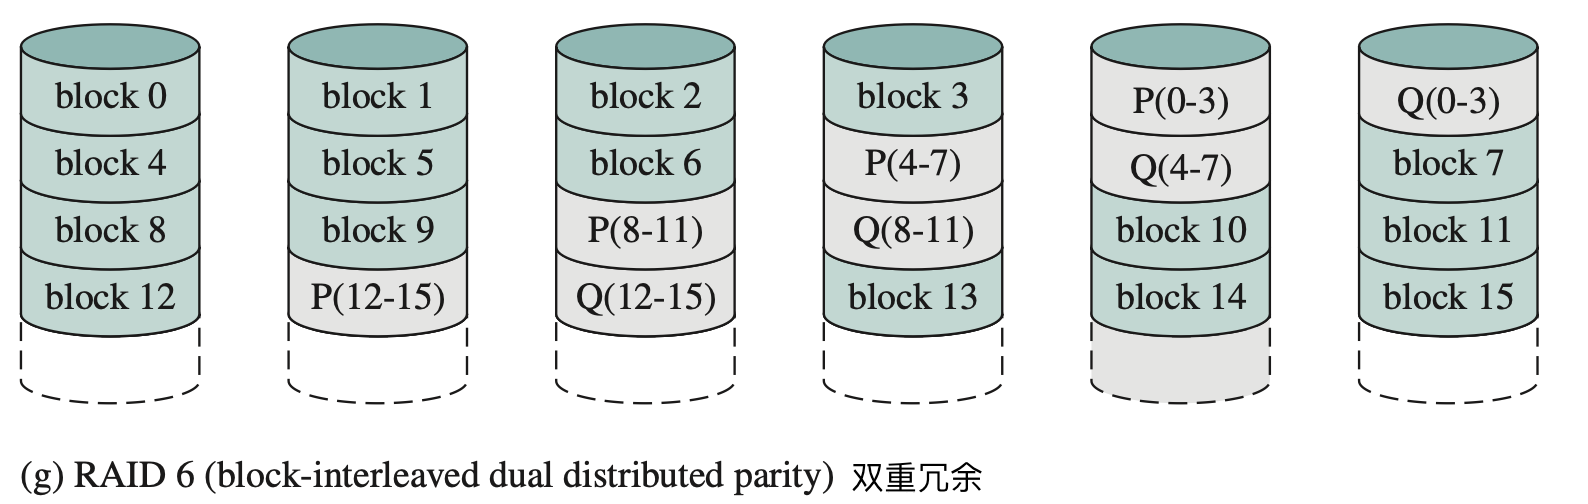
\includegraphics[width=0.8\textwidth]{img/RAID6}
	\end{figure}

	\subsubsection{RAID级别总结}
	\begin{table}[H]
		\centering
		\resizebox{\textwidth}{!}{
			\begin{threeparttable}
			\begin{tabular}{|c|c|c|c|c|c|c|}
				\hline
				类别                    & \begin{tabular}[c]{@{}c@{}}级\\ 别\end{tabular} & 说明                                                     & \begin{tabular}[c]{@{}c@{}}磁盘\\ 请求\tnote{*}\end{tabular} & 数据可用性                                                                  & 大I/O数据传送能力                                                            & 小I/O请求率                                                               \\ \hline
				条带化                   & 0                                             & 非冗余                                                    & $N$                                             & 低于单个磁盘                                                                 & 很高                                                                    & 读和写都很高                                                                \\ \hline
				镜像                    & 1                                             & 被镜像                                                    & $2N$                                            & \begin{tabular}[c]{@{}c@{}}高于 RAID 2、3、4 或\\ 5; 低于 RAID 6\end{tabular} & \begin{tabular}[c]{@{}c@{}}读时高于单个磁盘; \\ 写时与单个磁盘相近\end{tabular}        & \begin{tabular}[c]{@{}c@{}}读时最快为单磁盘2倍; \\ 写时与单磁盘相近\end{tabular}       \\ \hline
				\multirow{2}{*}{并行访问} & 2                                             & \begin{tabular}[c]{@{}c@{}}通过海明码\\ 实现冗余\end{tabular}   & $N+m$                                           & \begin{tabular}[c]{@{}c@{}}明显高于单个磁盘; 与\\ RAID 3、4或5可比\end{tabular}     & \begin{tabular}[c]{@{}c@{}}所有列出方案中最\\ 高的\end{tabular}                 & 约为单个磁盘的2倍                                                             \\ \cline{2-7} 
									  & 3                                             & \begin{tabular}[c]{@{}c@{}}交错位奇偶\\ 校验\end{tabular}     & $N+1$                                           & \begin{tabular}[c]{@{}c@{}}明显高于单个磁盘; 与\\ RAID 2、4或5可比\end{tabular}     & \begin{tabular}[c]{@{}c@{}}所有列出方案中最\\ 高的\end{tabular}                 & 约为单个磁盘的2倍                                                             \\ \hline
				\multirow{3}{*}{独立访问} & 4                                             & \begin{tabular}[c]{@{}c@{}}交错块奇偶\\ 校验\end{tabular}     & $N+1$                                           & \begin{tabular}[c]{@{}c@{}}明显高于单个磁盘; 与\\ RAID 2、3或5可比\end{tabular}     & \begin{tabular}[c]{@{}c@{}}读时与 RAID 0 相近;\\ 写时明显慢于单磁盘\end{tabular}    & \begin{tabular}[c]{@{}c@{}}读时与 RAID 0 相近;\\ 写时明显慢于单磁盘\end{tabular}    \\ \cline{2-7} 
									  & 5                                             & \begin{tabular}[c]{@{}c@{}}交错块分布\\ 奇偶校验\end{tabular}   & $N+1$                                           & \begin{tabular}[c]{@{}c@{}}明显高于单个磁盘; 与\\ RAID 2、3 或4可比\end{tabular}    & \begin{tabular}[c]{@{}c@{}}读时与 RAID 0 相近;\\ 写时明显慢于单磁盘\end{tabular}    & \begin{tabular}[c]{@{}c@{}}读时与 RAID 0 相近;\\ 写时明显慢于单磁盘\end{tabular}    \\ \cline{2-7} 
									  & 6                                             & \begin{tabular}[c]{@{}c@{}}交错块双重分\\ 布奇偶校验\end{tabular} & $N+2$                                           & 所有列出方案中最高的                                                             & \begin{tabular}[c]{@{}c@{}}读时与 RAID 0 相近;\\ 写时明显慢于RAID 5\end{tabular} & \begin{tabular}[c]{@{}c@{}}读时与 RAID 0 相近;\\ 写时明显慢于RAID 5\end{tabular} \\ \hline
				\end{tabular}

				\begin{tablenotes}
					\footnotesize
					\item[*] $N$ 表示数据磁盘数量,$m$ 与 $\log N$ 成比例
				\end{tablenotes}

			\end{threeparttable}
		}
		\end{table}

		\subsection{磁盘Cache}
		磁盘高速缓存是主存中为磁盘扇区设置的一个缓冲区,包含磁盘中某些扇区的副本

		利用局部性原理,可以减少平均存储器存取时间

		替换策略:
		\begin{itemize}
			\item 最近最少使用 LRU, Least Recently Used
			\begin{itemize}
				\item 替换在高速缓存中未被访问的时间最长的块
				\item 逻辑上高速缓存由一个关于块的栈组成,最近访问过的块在栈顶。当高速缓存中的一个块被访问到时,它从栈中当前的位置移到栈顶
				\item 当一个块从辅存中取入时,把位于栈顶的那一块移出,并把新到来的块压入栈顶
				\item 并不需要在主存中真正移动这些块,有一个栈指针与高速缓存相关联
			\end{itemize}
			\item 最不经常使用 LFU, Least Frequently Used
			\begin{itemize}
				\item 替换集合中被访问次数最少的块
				\item LFU 可以通过给每个块关联一个计数器来实现
				\item 当一个块被读入时,它的计数器被指定为 1;当每次访问到这一块时,它的计数器增 1
				\item 当需要替换时,选择计数器值最小的块
				\item 直觉上 LFU 比 LRU 更适合,因为 LFU 使用了关于每个块的更多的相关信息
			\end{itemize}
		\end{itemize}

		\section{虚拟设备}
		虚拟设备是用一类物理设备模拟另一类物理设备的技术,可以让独享型设备变为共享设备

		\subsection{SPOOLing系统的设计与实现}
		SPOOLing 软件是在内核外运行的系统 I/O 软件,采用预输入、缓输出和井管理技术,是多道程序设计系统中处理独占型设备的一种方法
		\begin{itemize}
			\item 通过创建守护进程和特殊目录解决独占型设备的空占问题
			\item 不仅设备利用率提高,作业的运行时间也会缩短,每个作业都感觉各自拥有所需的独占设备
		\end{itemize}

		为存放输入数据和输出数据,SPOOLing 系统在磁盘上开辟输入井和输出井
		\begin{itemize}
			\item “井”是用作缓冲的存储区域,采用井的技术能调节供求之间的矛盾,消除人工干预带来的损失
		\end{itemize}

		SPOOLing 系统的组成
		\begin{itemize}
			\item 预输入程序:将数据从输入设备传送到磁盘输入井
			\begin{itemize}
				\item 操作系统将一批作业从输入设备上预先输入到磁盘的输入缓冲区中暂时保存,这称为“预输入”
				\item 调度作业执行时,作业使用数据不必再启动输入设备,从磁盘的输入缓冲区读入即可
			\end{itemize}
			\item 缓输出程序:将数据从磁盘输出井传送到输出设备
			\begin{itemize}
				\item 作业执行中不必直接启动输出设备,只要将作业的输出数据暂时保存到磁盘的输出缓冲区
				\item 当作业执行完毕后,由操作系统组织信息成批输出
			\end{itemize}
			\item 井管理程序:控制作业和井之间的数据交换
			\begin{itemize}
				\item 放置在井中的文件被称为井文件,井文件空间管理简单,它被划分为等长的的物理块,每块用来存放一条或多条逻辑记录
			\end{itemize}
		\end{itemize}
		\begin{figure}[H]
			\centering
			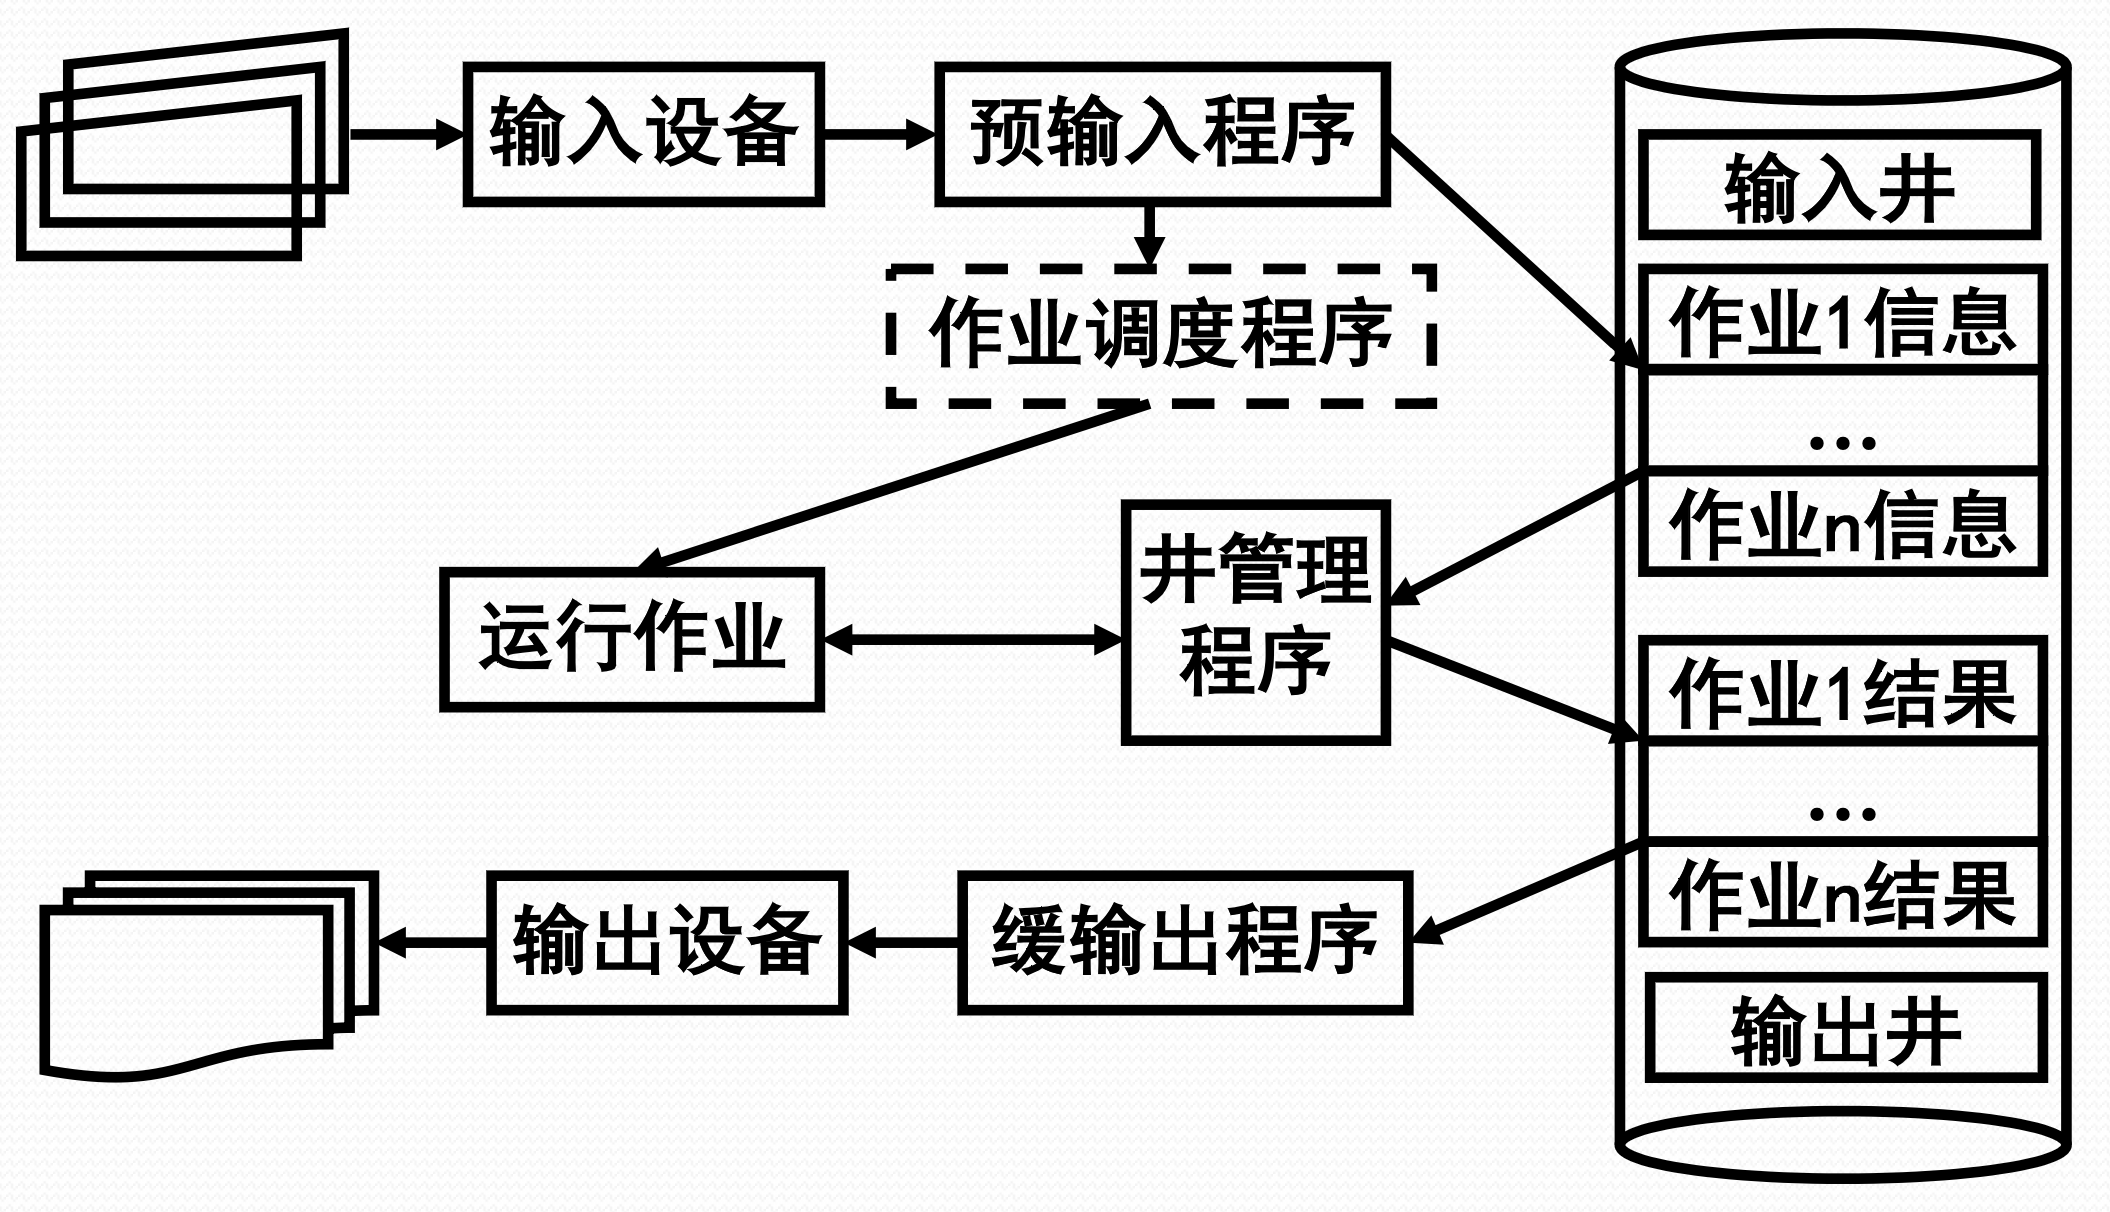
\includegraphics[width=0.65\textwidth]{img/4.5.1}
		\end{figure}

		\subsection{输入井的作业状态}
		\begin{itemize}
			\item 输入状态:正在预输入
			\item 收容状态:预输入完成,等待执行
			\item 执行状态:作业选中执行,正在从输入井读取输入,向输出井写入数据
			\item 完成状态:作业已经撤离,输出结果等待缓输出
			\item 通过预处理,结合井管理,可以实现为脱机状态,从联机(online)到脱机(offline),成功耦合
		\end{itemize}
		
		\begin{figure}[H]
			\centering
			\subfloat{
				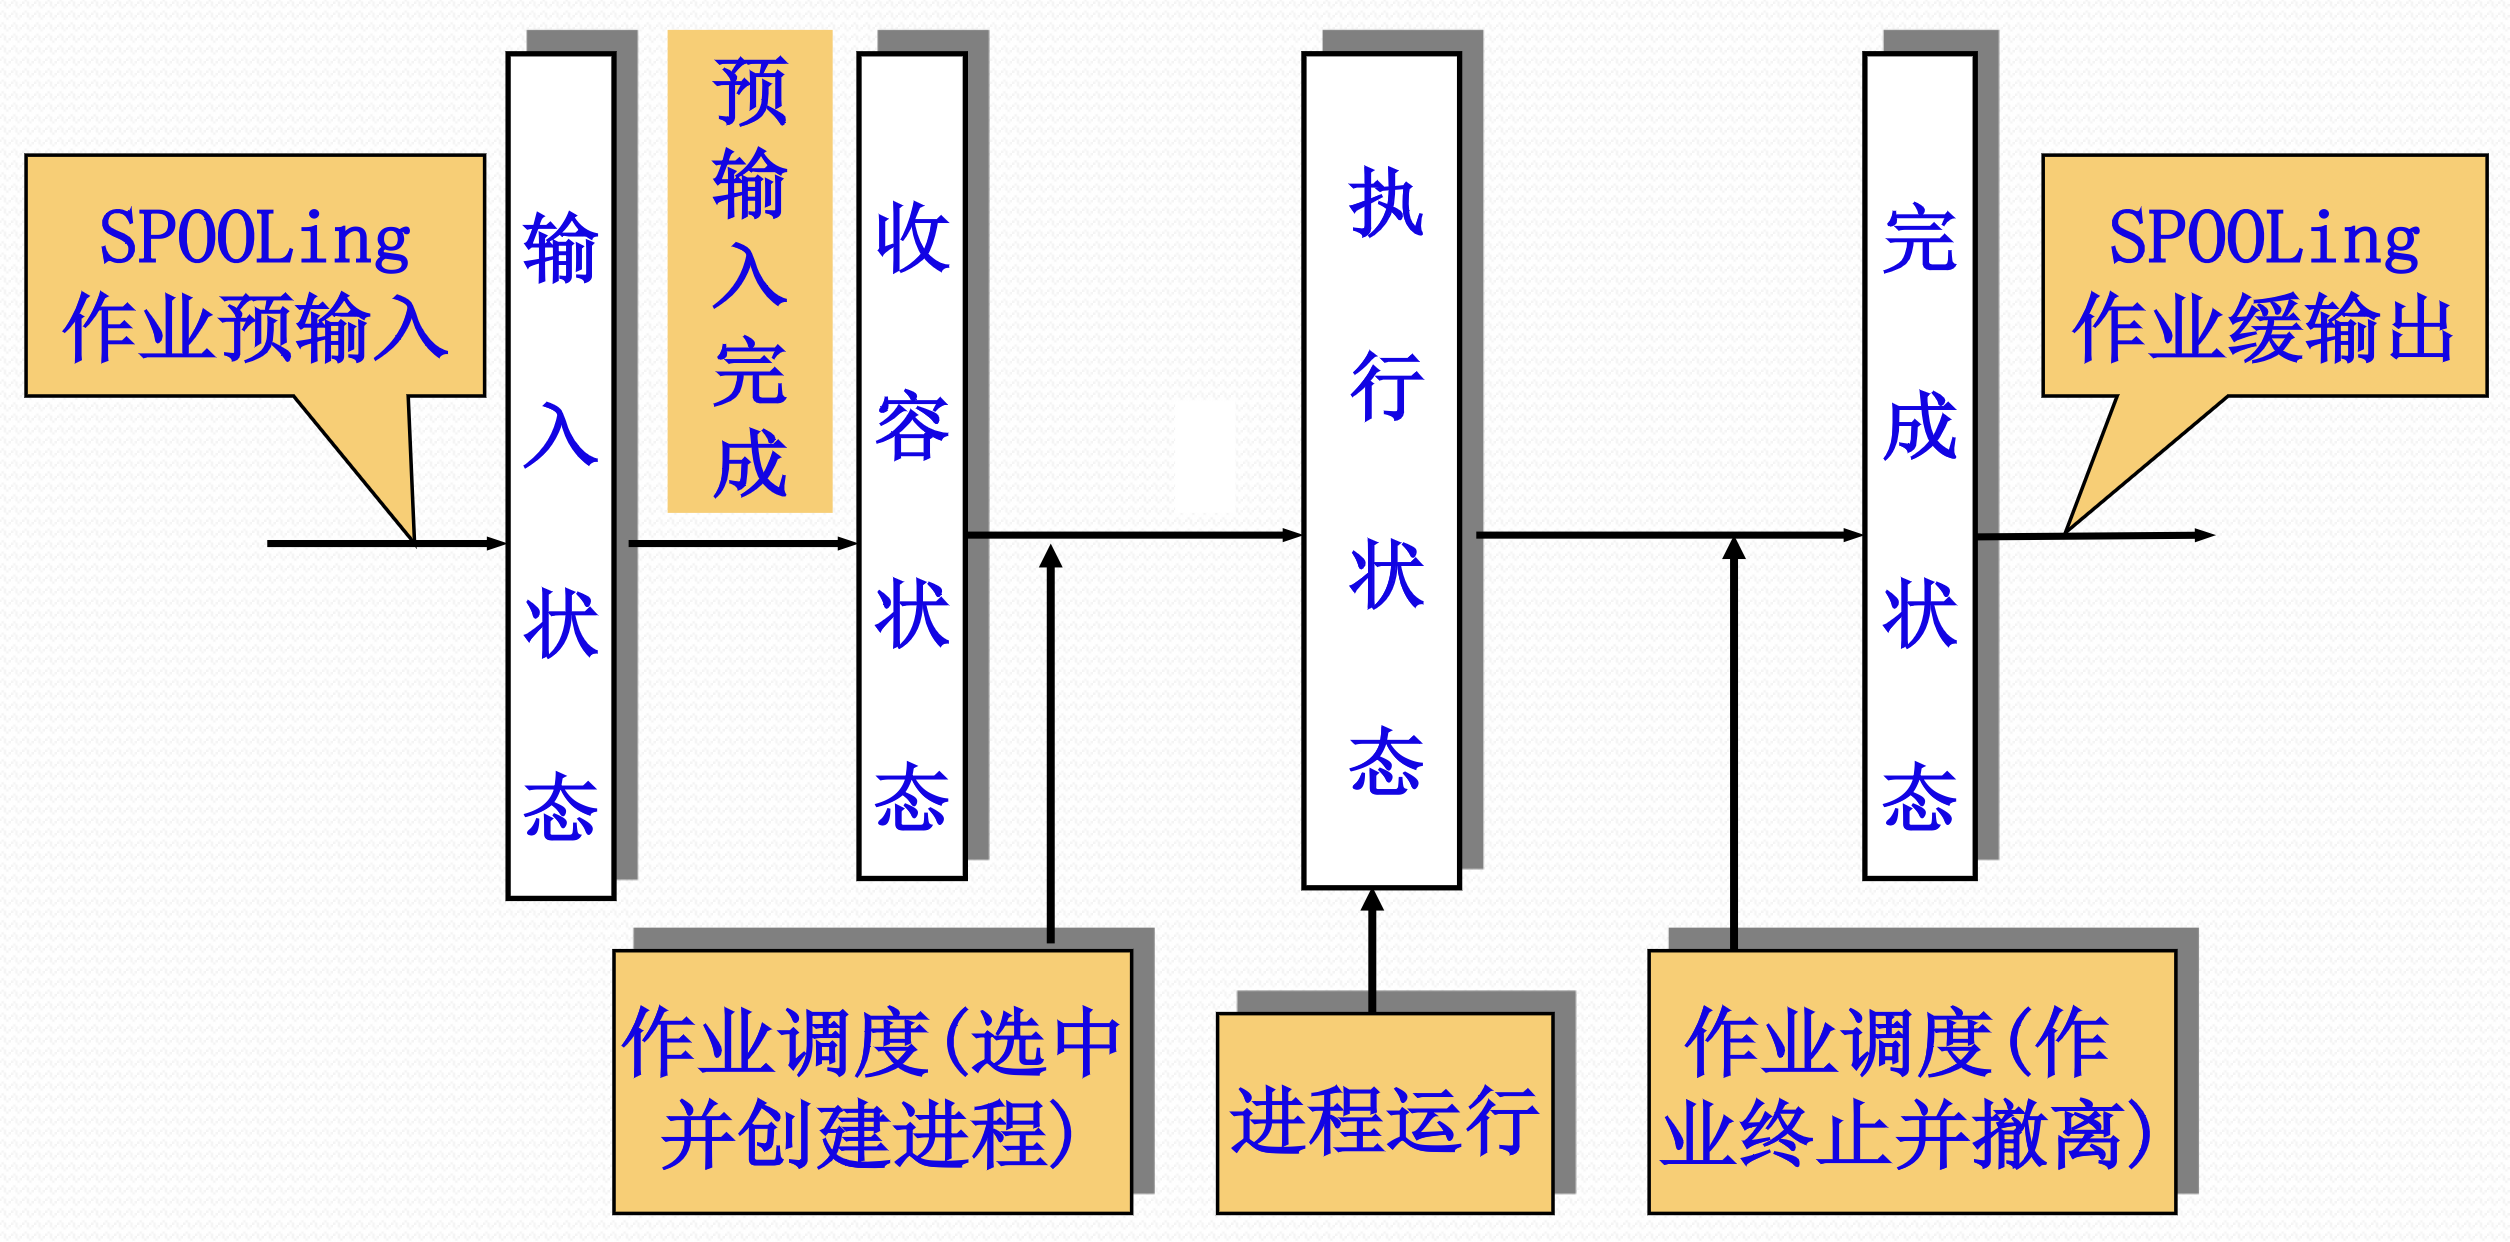
\includegraphics[width=0.45\textwidth]{img/4.5.2.1}
			}
			\subfloat{
				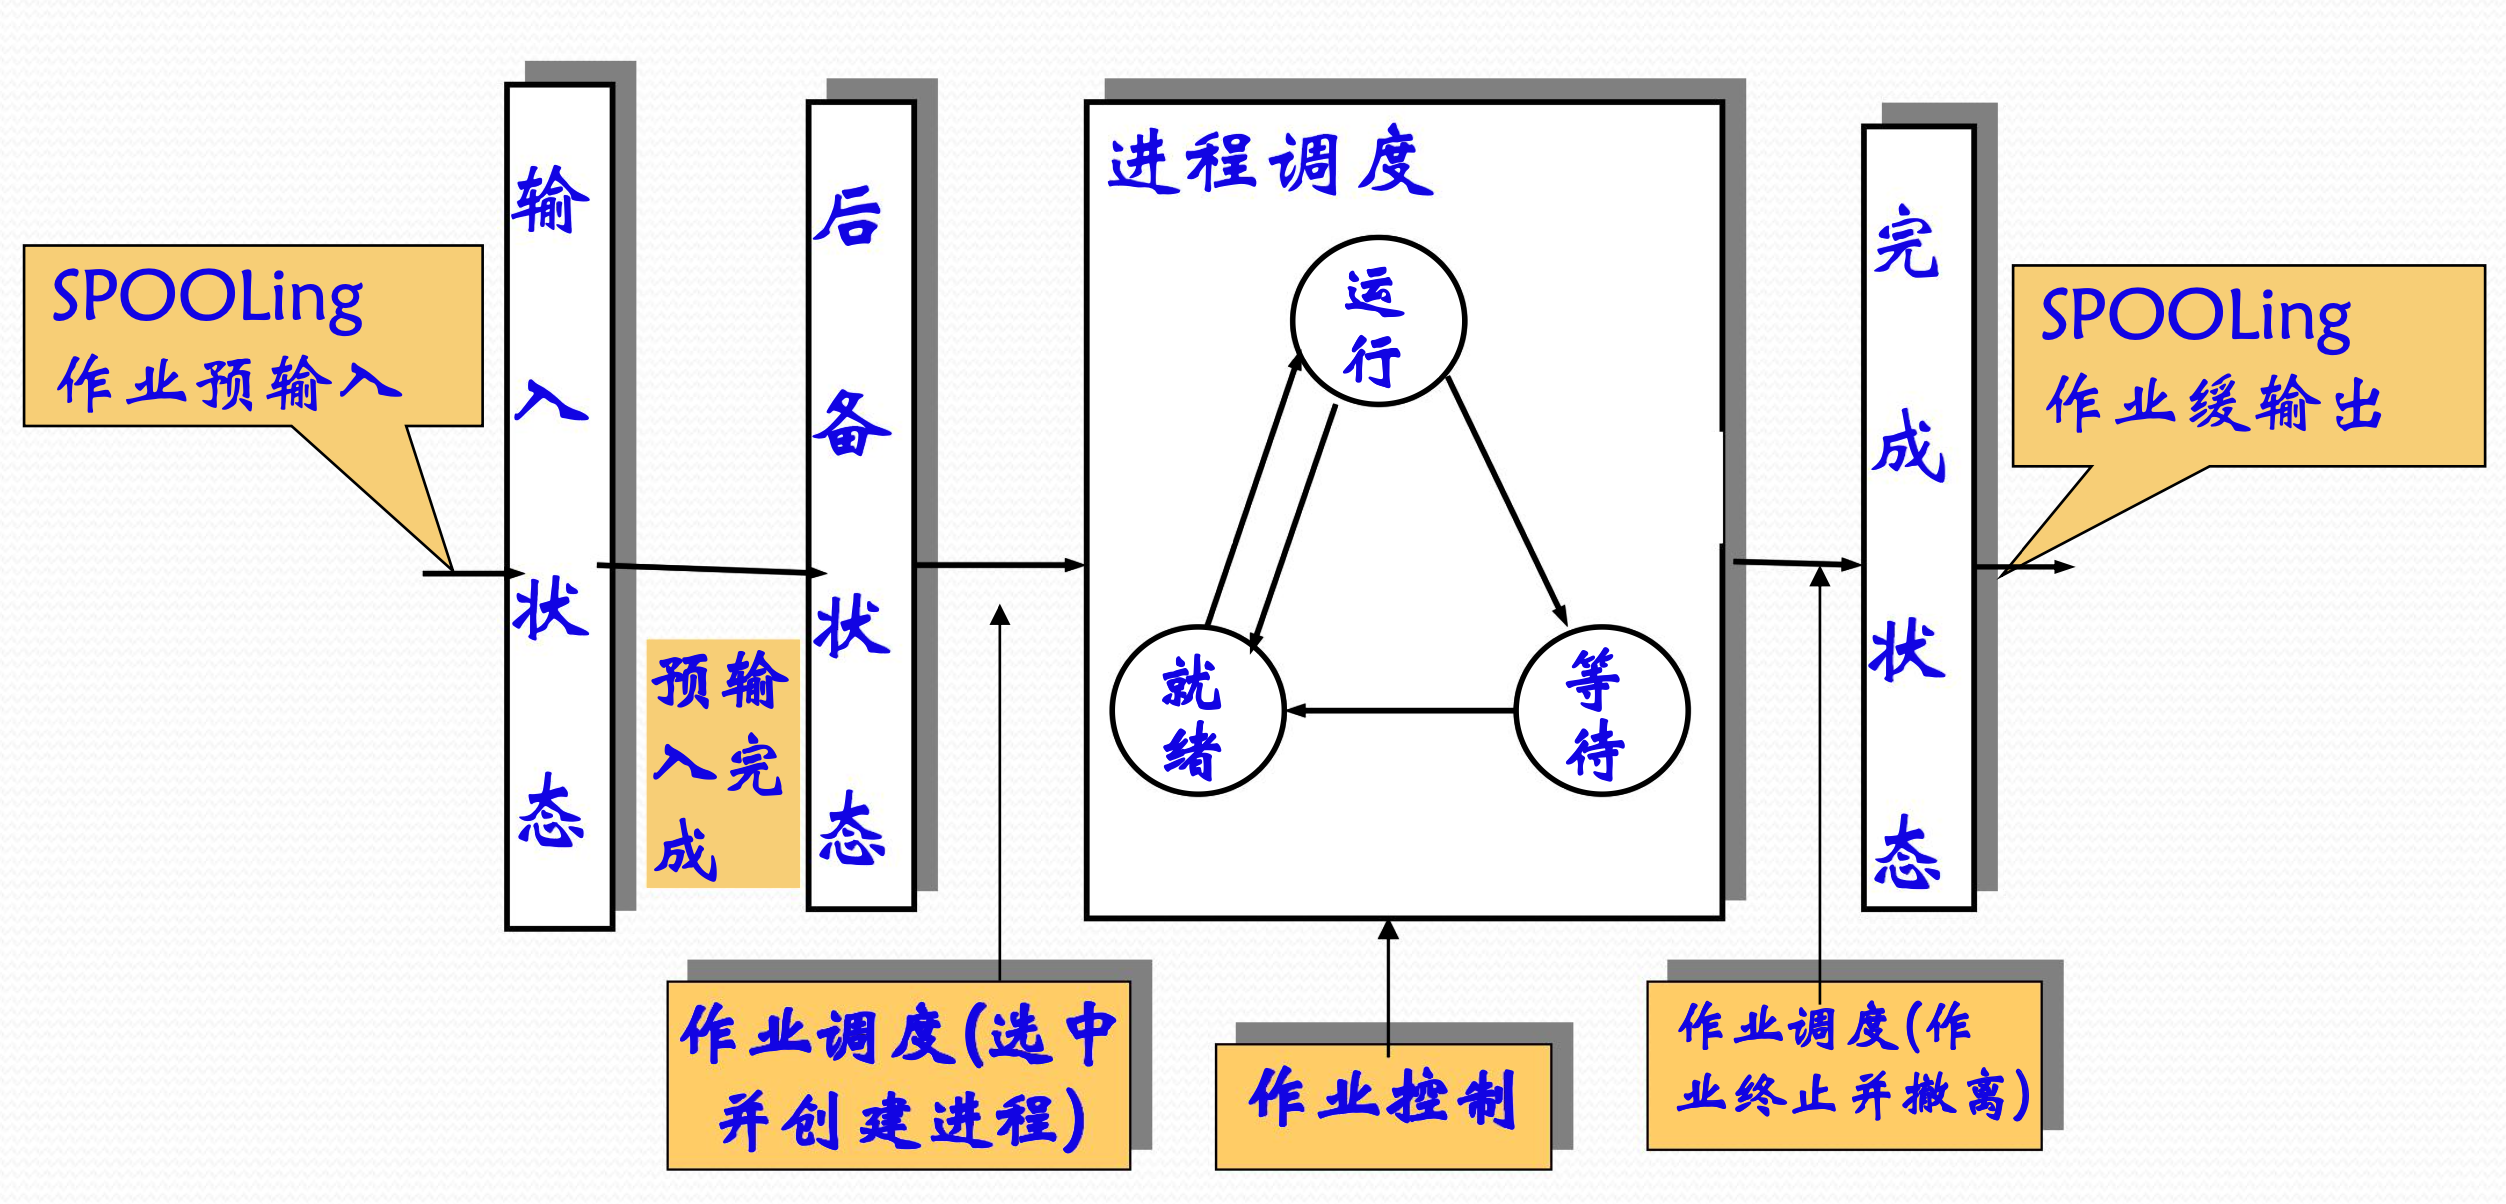
\includegraphics[width=0.48\textwidth]{img/4.5.2.2}
			}
		\end{figure}

		\subsection{打印机SPOOLing}
		打印机 SPOOLing 守护进程是一个典型的 SPOOLing 应用
		\begin{itemize}
			\item 解决的问题:打印机空占问题
			\begin{itemize}
				\item 如果用户进程通过打开打印机的设备文件来申请和使用打印机,往往会造成该进程打开设备文件后长达数小时不用,但其他进程又无法使用打印机
			\end{itemize}
			\item 打印机守护进程和 SPOOLing 打印目录
			\begin{itemize}
				\item 守护进程是唯一有特权使用打印机设备的进程
				\item 打印文件前,用户进程先产生完整的待输出文件,并存放在打印目录下
				\item 打印机空闲时,启动守护进程,打印待输出文件
			\end{itemize}
		\end{itemize}

\end{document}


